\documentclass[table]{beamer}

\usepackage{pucv_jz}

\title{Variables Aleatorias}
\subtitle{Estadística Computacional}
\author[J.Z.O-2023]{Juan Zamora Osorio\\\url{juan.zamora@pucv.cl}}
\institute[PUCV]{Instituto de Estadística\\Pontificia Universidad Cat\'olica de Valpara\'iso}
\date{\today}

\begin{document}

\frame{\titlepage}



\begin{frame}
    \frametitle{Variables Aleatorias -- cantidad de cartas negras}
    \begin{block}{Sacando una carta -- posibilidades}
        \begin{center}
            \begin{tabular}{c|c}
                $\clubsuit$ & 1 \\
                $\diamondsuit$ & 0 \\
                $\heartsuit$ & 0 \\
                $\spadesuit$ & 1
            \end{tabular}
        \end{center}
    \end{block}
    \begin{block}{Sacando una carta -- probabilidades}
        \begin{center}
            \begin{tabular}{c|c|c}
                Cantidad negras & 0 & 1 \\
                \hline
                Probabilidad & $\frac{2}{4} = \frac{1}{2}$ & $\frac{2}{4} = \frac{1}{2}$
            \end{tabular}
        \end{center}
    \end{block}
\end{frame}

\begin{frame}
    \frametitle{Variables Aleatorias -- cantidad de cartas negras}
    \begin{block}{Sacando dos cartas -- posibilidades}
        \begin{center}
            \begin{tabular}{c|cccc}
                & $\clubsuit$ & $\diamondsuit$ & $\heartsuit$ & $\spadesuit$ \\
                \hline
                $\clubsuit$ & 2 & 1 & 1 & 2 \\
                $\diamondsuit$ & 1 & 0 & 0 & 1 \\
                $\heartsuit$ & 1 & 0 & 0 & 1 \\
                $\spadesuit$ & 2 & 1 & 1 & 2
            \end{tabular}
        \end{center}
    \end{block}
    \begin{block}{Sacando dos cartas -- probabilidades}
        \begin{center}
            \begin{tabular}{c|c|c|c}
                Cantidad negras & 0 & 1 & 2 \\
                \hline
                Probabilidad & $\frac{4}{16} = \frac{1}{4}$ &
                $\frac{8}{16} = \frac{1}{2}$ &
                $\frac{4}{16} = \frac{1}{4}$
            \end{tabular}
        \end{center}
    \end{block}
\end{frame}


\begin{frame}
    \frametitle{Variables Aleatorias -- cantidad de cartas negras}
    \begin{block}{Sacando tres cartas -- posibilidades}
        \begin{center}
            \small
            \begin{tabular}{c|cccc}
                $\clubsuit$ & $\clubsuit$ & $\diamondsuit$ & $\heartsuit$ & $\spadesuit$ \\
                \hline
                $\clubsuit$ & 3 & 2 & 2 & 3 \\
                $\diamondsuit$ & 2 & 1 & 1 & 2 \\
                $\heartsuit$ & 2 & 1 & 1 & 2 \\
                $\spadesuit$ & 3 & 2 & 2 & 3
            \end{tabular}
            \begin{tabular}{c|cccc}
                $\diamondsuit$ & $\clubsuit$ & $\diamondsuit$ & $\heartsuit$ & $\spadesuit$ \\
                \hline
                $\clubsuit$ & 2 & 1 & 1 & 2 \\
                $\diamondsuit$ & 1 & 0 & 0 & 1 \\
                $\heartsuit$ & 1 & 0 & 0 & 1 \\
                $\spadesuit$ & 2 & 1 & 1 & 2
            \end{tabular}
        \end{center}
        \begin{center}
            \small
            \begin{tabular}{c|cccc}
                $\heartsuit$ & $\clubsuit$ & $\diamondsuit$ & $\heartsuit$ & $\spadesuit$ \\
                \hline
                $\clubsuit$ & 2 & 1 & 1 & 2 \\
                $\diamondsuit$ & 1 & 0 & 0 & 1 \\
                $\heartsuit$ & 1 & 0 & 0 & 1 \\
                $\spadesuit$ & 2 & 1 & 1 & 2 \\
            \end{tabular}
            \begin{tabular}{c|cccc}
                $\spadesuit$ & $\clubsuit$ & $\diamondsuit$ & $\heartsuit$ & $\spadesuit$ \\
                \hline
                $\clubsuit$ & 3 & 2 & 2 & 3 \\
                $\diamondsuit$ & 2 & 1 & 1 & 2 \\
                $\heartsuit$ & 2 & 1 & 1 & 2 \\
                $\spadesuit$ & 3 & 2 & 2 & 3
            \end{tabular}
        \end{center}
    \end{block}
    \begin{block}{Sacando tres cartas -- probabilidades}
        \begin{center}
            \begin{tabular}{c|c|c|c|c}
                Cantidad negras & 0 & 1 & 2 & 3 \\
                \hline
                Probabilidad & $\frac{8}{64} = \frac{1}{8}$ &
                $\frac{24}{64} = \frac{3}{8}$ &
                $\frac{24}{64} = \frac{3}{8}$ &
                $\frac{8}{64} = \frac{1}{8}$
            \end{tabular}
        \end{center}
    \end{block}
\end{frame}


%%%

\begin{frame}
    \frametitle{Variables Aleatorias -- definición}
    \begin{block}{Formalmente}
        \begin{itemize}
            \item Función \emph{medible} entre un espacio muestral $\Omega$ y otro $\Omega'$:
                \begin{equation*}
                    X : \Omega \rightarrow \Omega' .
                \end{equation*}
            \item La preimagen de todo conjunto en el espacio de eventos asociado a $\Omega'$ es un conjunto en el espacio de eventos de $\Omega$.
        \end{itemize}
    \end{block}
    \begin{exampleblock}{Ejemplo}
        \begin{itemize}
            \item $X$ cantidad de cartas negras al sacar 3 cartas independientes.
            \item $\Omega' = \bparens{0, 1, 2, 3}$.
            \item $\Omega = \bparens{\parens{\clubsuit, \clubsuit, \clubsuit},
                    \parens{\clubsuit, \clubsuit, \diamondsuit},
                    \parens{\clubsuit, \clubsuit, \heartsuit},
                    \parens{\clubsuit, \clubsuit, \spadesuit},
                    \parens{\clubsuit, \diamondsuit, \clubsuit},
                    \ldots, }$.
                    % \parens{\spadesuit, \spadesuit, \spadesuit}}$.
            \item $X \parens{\parens{\clubsuit, \diamondsuit, \clubsuit}} = 2$.
        \end{itemize}
    \end{exampleblock}
\end{frame}

\begin{frame}
    \frametitle{En este curso}
    \begin{block}{$X : \Omega \rightarrow E$}
        \begin{itemize}
            \item Si $E$ es finito o numerable: variable aleatoria discreta.
            \item Si $E \subseteq \reals$ no numerable: variable aleatoria continua.
        \end{itemize}
    \end{block}
    \begin{center}
        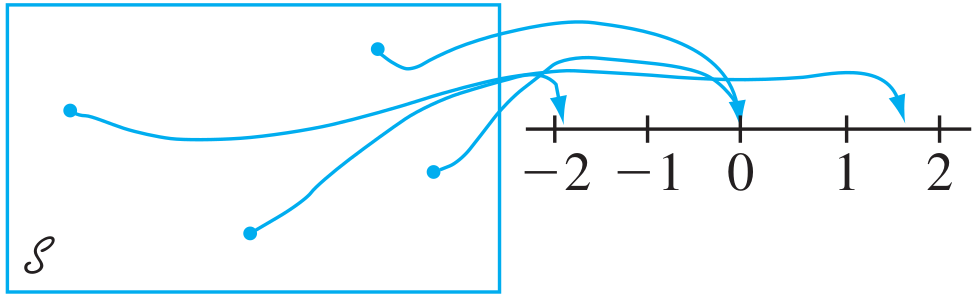
\includegraphics[width=0.45\textwidth]{varaleat_devore}
    \end{center}
    \begin{exampleblock}{Ejemplo -- variable aleatoria discreta}
        \begin{itemize}
            \item $X$ cantidad de cartas negras al sacar 3 cartas independientes.
        \end{itemize}
    \begin{center}
        \begin{tabular}{c|c}
            Cantidad negras & Probabilidad \\
            \hline
            0 & $0.125$ \\
            1 & $0.375$ \\
            2 & $0.375$ \\
            3 & $0.125$
        \end{tabular}
    \end{center}
    \end{exampleblock}
\end{frame}


%%

\begin{frame}
    \frametitle{Notación}
    \begin{block}{$X : \Omega \rightarrow E$}
        \begin{itemize}
            \item Sea $S \subseteq E$, $\pprob{X}{S} = \prob{X \in S} = \prob{X^{-1} \parens{S}} = \prob{\bparens{\omega \in \Omega : X \parens{\omega} \in S}}$.
            \item $P_{X}$:
                \begin{itemize}
                    \item Distribución de probabilidad.
                    \item Ley de probabilidad.
                \end{itemize}
        \end{itemize}
    \end{block}
    \begin{exampleblock}{Ejemplo -- variable aleatoria discreta}
        \begin{itemize}
            \item $\pprob{X}{\bparens{0, 1}} = \prob{\bparens{\diamondsuit \diamondsuit \diamondsuit, \diamondsuit \heartsuit \clubsuit, \spadesuit \diamondsuit \heartsuit, \spadesuit \heartsuit \heartsuit, \diamondsuit \clubsuit \heartsuit, \diamondsuit \diamondsuit \heartsuit , \ldots}}$.
        \end{itemize}
    \begin{center}
        \begin{tabular}{c|c}
            $X$ & $P_{X}$ \\
            \hline
            0 & $0.125$ \\
            1 & $0.375$ \\
            2 & $0.375$ \\
            3 & $0.125$
        \end{tabular}
    \end{center}
    \end{exampleblock}
\end{frame}

\begin{frame}
    \frametitle{Variables aleatorias discretas}
    \begin{block}{Función de masa de probabilidad (\emph{pmf})}
        \begin{equation*}
            \ff{x} = \prob{X = x} = \pprob{X}{\bparens{x}} .
        \end{equation*}
    \end{block}
    \begin{block}{Recordar de probabilidades ($\Omega$ finito)}
        \begin{equation*}
            \ff{x} = \prob{X = x} = \frac{n_{x}}{n} = \frac{\vparens{X^{-1} \parens{\bparens{x}}}}{\vparens{\Omega}}.
        \end{equation*}
        \begin{itemize}
            \item $n_{x}$ cantidad de resultados $\omega$ que cumplen $X \parens{\omega} = x$.
            \item $n$ cantidad de resultados en $\Omega$.
        \end{itemize}
    \end{block}
\end{frame}

\begin{frame}
    \frametitle{Ejemplo: moneda lanzada 3 veces}
    \begin{exampleblock}{Ejemplo 1}
        \begin{itemize}
            \item $X$ cantidad de caras.
            \item Posibles valores: $\bparens{0, 1, 2, 3}$.
        \end{itemize}
    \end{exampleblock}
    \begin{center}
        \begin{tabular}{ccc}
            $x$ & $X^{-1} \parens{\bparens{x}}$ & $\prob{X = x}$ \\
            \hline
            0 & $\bparens{sss}$ & $\frac{1}{8} = 0.125$ \\
            1 & $\bparens{css, scs, ssc}$ & $\frac{3}{8} = 0.375$ \\
            2 & $\bparens{ccs, csc, scc}$ & $\frac{3}{8} = 0.375$ \\
            3 & $\bparens{ccc}$ & $\frac{1}{8} = 0.125$
        \end{tabular}
    \end{center}
\end{frame}

%%%%

\begin{frame}
    \frametitle{Ejemplo: moneda lanzada 3 veces}
    \begin{exampleblock}{Ejemplo 2}
        \begin{itemize}
            \item $X$ string de bits 0/1 según cara/sello obtenido.
            \item Posibles valores: $\bparens{000, 001, 010, 011, 100, 101, 110, 111}$.
        \end{itemize}
    \end{exampleblock}
    \begin{center}
        \begin{tabular}{ccc}
            $x$ & $X^{-1} \parens{\bparens{x}}$ & $\prob{X = x}$ \\
            \hline
            000 & $\bparens{ccc}$ & $\frac{1}{8} = 0.125$ \\
            001 & $\bparens{ccs}$ & $\frac{1}{8} = 0.125$ \\
            010 & $\bparens{csc}$ & $\frac{1}{8} = 0.125$ \\
            011 & $\bparens{css}$ & $\frac{1}{8} = 0.125$ \\
            100 & $\bparens{scc}$ & $\frac{1}{8} = 0.125$ \\
            101 & $\bparens{scs}$ & $\frac{1}{8} = 0.125$ \\
            110 & $\bparens{ssc}$ & $\frac{1}{8} = 0.125$ \\
            111 & $\bparens{sss}$ & $\frac{1}{8} = 0.125$
        \end{tabular}
    \end{center}
\end{frame}

\begin{frame}
    \frametitle{Ejemplo: moneda lanzada 3 veces}
    \begin{exampleblock}{Ejemplo 3}
        \begin{itemize}
            \item $X$ cantidad de caras par o impar.
            \item Posibles valores: $\bparens{P, I} \equiv \bparens{0, 1}$.
        \end{itemize}
    \end{exampleblock}
    \begin{center}
        \begin{tabular}{ccc}
            $x$ & $X^{-1} \parens{\bparens{x}}$ & $\prob{X = x}$ \\
            \hline
            $P \equiv 0$ & $\bparens{ccs, csc, scc, sss}$ & $\frac{1}{2} = 0.5$ \\
            $I \equiv 1$ & $\bparens{ccc, css, scs, ssc}$ & $\frac{1}{2} = 0.5$
        \end{tabular}
    \end{center}
\end{frame}

\begin{frame}
    \frametitle{Función de distribución acumulada (\emph{cdf})}
    \begin{block}{Definición}
        \begin{equation*}
            F : \reals \rightarrow \sparens{0, 1} \text{ tal que }
            \FF{x} = \prob{X \leq x} .
        \end{equation*}
    \end{block}
    \begin{block}{Variables aleatorias discretas}
        \begin{equation*}
            \FF{x} = \prob{X \leq x} = \sum_{y \leq x} \prob{X = y} = \sum_{y \leq x} \ff{y} .
        \end{equation*}
    \end{block}
    \begin{block}{Propiedades}
        \begin{itemize}
            \item $F$ es no decreciente ($x_{1} \leq x_{2} \Rightarrow \FF{x_{1}} \leq \FF{x_{2}}$).
            \item $\lim_{x \rightarrow - \infty} \FF{x} = 0$.
            \item $\lim_{x \rightarrow + \infty} \FF{x} = 1$.
            \item $\forall x , 0 \leq \FF{x} \leq 1$.
            \item Está definida para todo $\reals$.
        \end{itemize}
    \end{block}
\end{frame}

\begin{frame}
    \frametitle{Función de distribución acumulada (\emph{cdf})}
    \begin{exampleblock}{Ejemplo: Cantidad de caras al lanzar 4 monedas}
        \begin{center}
            \begin{tabular}{c|c|c}
                $x$ & $\ff{x} = \prob{X = x}$ & $\FF{x} = \sum_{y \leq x} \ff{y}$ \\
                \hline
                0 & $\frac{1}{16} = 0.0625$ & $\frac{1}{16} = 0.0625$ \\
                1 & $\frac{4}{16} = 0.25$ & $\frac{5}{16} = 0.3125$ \\
                2 & $\frac{6}{16} = 0.375$ & $\frac{11}{16} = 0.6875$ \\
                3 & $\frac{4}{16} = 0.25$ & $\frac{15}{16} = 0.9375$ \\
                4 & $\frac{1}{16} = 0.0625$ & $\frac{16}{16} = 1$
            \end{tabular}
        \end{center}
    \end{exampleblock}
    \begin{center}
        \begin{tabular}{cc}
            \emph{pmf} ($\ff{x}$) & \emph{cdf} ($\FF{x}$) \\
            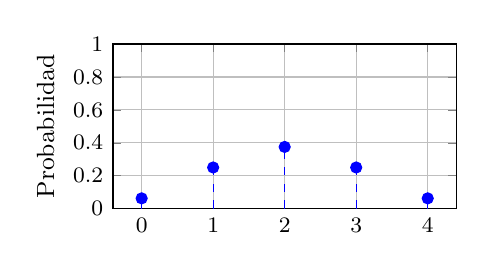
\begin{tikzpicture}
                \begin{axis}[
                    footnotesize,
                    %clip=false,
                    %domain=-2:2,
                    ymin=0,
                    ymax=1,
                    ylabel=Probabilidad,
                    height=0.49\textwidth/1.618,
                    width=0.49\textwidth,
                    xtick distance=1,
                    %axis lines=middle,
                    grid=major,
                    %no markers,
                    ]
                    \addplot+[forget plot, dashed, no markers] coordinates {(0, 0) (0, 1/16)};
                    \addplot+[forget plot, dashed, no markers] coordinates {(1, 0) (1, 4/16)};
                    \addplot+[forget plot, dashed, no markers] coordinates {(2, 0) (2, 6/16)};
                    \addplot+[forget plot, dashed, no markers] coordinates {(3, 0) (3, 4/16)};
                    \addplot+[forget plot, dashed, no markers] coordinates {(4, 0) (4, 1/16)};
                    \addplot+[only marks] coordinates {(0, 1/16) (1, 4/16) (2, 6/16) (3, 4/16) (4, 1/16)};
                \end{axis}
            \end{tikzpicture}
            &
            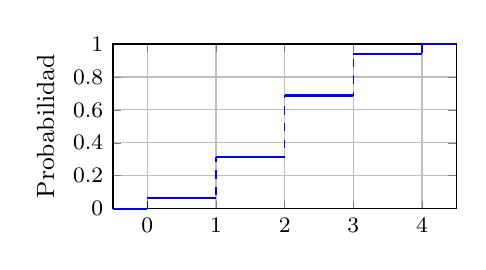
\begin{tikzpicture}
                \begin{axis}[
                    footnotesize,
                    clip=false,
                    %domain=-2:2,
                    ymin=0,
                    ymax=1,
                    xmin=-0.5,
                    xmax=4.5,
                    xtick distance=1,
                    ylabel=Probabilidad,
                    height=0.49\textwidth/1.618,
                    width=0.49\textwidth,
                    %axis lines=middle,
                    grid=major,
                    no markers,
                    ]
                    \addplot+[forget plot, dashed, const plot] coordinates {(-0.5, 0) (0, 1/16) (1, 5/16) (2, 11/16) (3, 15/16) (4, 1) (4.5, 1)};
                    \addplot+[thick, jump mark left] coordinates {(-0.5, 0) (0, 1/16) (1, 5/16) (2, 11/16) (3, 15/16) (4, 1) (4.5, 1)};
                \end{axis}
            \end{tikzpicture}
        \end{tabular}
    \end{center}
\end{frame}

\begin{frame}
    \frametitle{Esperanza -- valor esperado -- media}
    \begin{block}{Definición}
        \begin{equation*}
            \expecteddist{X \sim f}{X} = \mu_{X} = \sum_{x \in E} x \ff{x} .
        \end{equation*}
    \end{block}
    \begin{exampleblock}{Ejemplo: Cantidad de caras al lanzar 4 monedas}
        %\begin{itemize}
          %  \item Cantidad de caras al lanzar 4 monedas:
                \begin{equation*}
                    \expected{X} = \frac{1}{16} 0 + \frac{4}{16} 1 + \frac{6}{16} 2 + \frac{4}{16} 3 + \frac{1}{16} 4 = 2 .
                \end{equation*}
%            \item Cantidad de personas sanas cuando llega primera con COVID-19:
%                \begin{equation*}
%                    \expected{X} = \sum_{x = 0}^{\infty} x \parens{1 - p}^{x} p = \frac{1 - p}{p} .
%                \end{equation*}
%            \item Cantidad de personas con COVID-19 en reunión de $n$ personas:
%                \begin{equation*}
%                    \expected{X} = \sum_{x = 0}^{n} x \binom{n}{x} p^{x} \parens{1 - p}^{n - x} = n p .
%                \end{equation*}
        %\end{itemize}
    \end{exampleblock}
\end{frame}

\begin{frame}
    \frametitle{Esperanza -- valor esperado -- media}
    \begin{block}{Definición}
        \begin{itemize}
            \item Sea $g : E \rightarrow \reals$ una función:
                \begin{equation*}
                    \expecteddist{X \sim f}{g \parens{X}} = \sum_{x \in E} g \parens{x} \ff{x} .
                \end{equation*}
        \end{itemize}
    \end{block}
    \begin{block}{Propiedades: linealidad}
        \begin{itemize}
            \item Sean $a, b \in \reals$:
                \begin{equation*}
                    \expected{a X + b} = a \expected{X} + b .
                \end{equation*}
            \item Sean $g_{1}, g_{2} : E \rightarrow \reals$ funciones:
                \begin{equation*}
                    \expected{g_{1} \parens{X} + g_{2} \parens{X}} = \expected{g_1 \parens{X}} + \expected{g_{2} \parens{X}} .
                \end{equation*}
        \end{itemize}
    \end{block}
\end{frame}

\begin{frame}
    \frametitle{Varianza}
    \begin{block}{Definición}
        \begin{equation*}
            \variancedist{X \sim f}{X} = \sigma^{2}_{X} = \expecteddist{X \sim f}{\parens{X - \mu_{X}}^{2}} = \sum_{x \in E} \parens{x - \mu_{X}}^{2} \ff{x} .
        \end{equation*}
    \end{block}
    \begin{block}{Desviación estándar}
        \begin{equation*}
            \sigma_{X} = \sqrt{\sigma_{X}^{2}} = \sqrt{\variancedist{X \sim f}{X}} .
        \end{equation*}
    \end{block}
    \begin{block}{Propiedad}
        \begin{equation*}
            \variancedist{X \sim f}{X} = \sigma^{2}_{X} = \expecteddist{X \sim f}{X^{2}} - \expecteddist{X \sim f}{X}^{2}
            = \sparens{\sum_{x \in E} x^{2} \ff{x}} - \mu_{X}^{2} .
        \end{equation*}
    \end{block}
\end{frame}

\begin{frame}
    \frametitle{Varianza}
    \begin{block}{Definición}
        \begin{itemize}
            \item Sea $g : E \rightarrow \reals$ una función:
                \begin{equation*}
                    \variancedist{X \sim f}{g \parens{X}} = \sum_{x \in E} \parens{g \parens{x} - \expecteddist{X \sim f}{g \parens{X}}}^{2} \ff{x} .
                \end{equation*}
        \end{itemize}
    \end{block}
    \begin{block}{Propiedad: no linealidad}
        \begin{itemize}
            \item Sean $a, b \in \reals$:
                \begin{equation*}
                    \variance{a X + b} = a^{2} \variance{X} .
                \end{equation*}
        \end{itemize}
    \end{block}
\end{frame}

\begin{frame}
    \frametitle{Distribución $X \sim \bernoulli{p}$}
    \begin{block}{Definición}
            \begin{equation*}
                \ff{x} = \begin{cases} p \text{ si } x = 1, \\ 1 - p \text{ si } x = 0. \end{cases}
            \end{equation*}
    \end{block}
    \begin{exampleblock}{Ejemplos}
        \begin{itemize}
            \item Lanzar una moneda.
            \item Ser fiscalizado en carretera.
        \end{itemize}
    \end{exampleblock}
    \begin{block}{Propiedades}
        \begin{itemize}
            \item $\expecteddist{X \sim \bernoulli{p}}{X} = \mu_{X} = p$.
            \item $\variancedist{X \sim \bernoulli{p}}{X} = \sigma^{2}_{X} = p \parens{1 - p}$.
        \end{itemize}
    \end{block}
\end{frame}

\begin{frame}
    \frametitle{Ejemplo: Reunión de personas sin COVID-19}
    \begin{block}{Supuestos}
        \begin{itemize}
            \item Reunión de personas, van llegando de a una.
            \item Cada persona que llega tiene probabilidad $p$ de tener COVID-19.
            \item Probabilidad $p$ es independiente entre personas.
            \item $X-1$ cantidad de personas sanas cuando llega primera con COVID-19 (Igual cantidad total de personas menos 1)
        \end{itemize}
    \end{block}
    \begin{center}
        \begin{tabular}{c|c|c|c}
            $x$ & Evento & $\ff{x} = \prob{X = x}$ & $\FF{x} = \sum_{y \leq x} \ff{y}$ \\
            \hline
            1 & $\bparens{c \ldots}$ & $p$ & $p$ \\
            2 & $\bparens{nc \ldots}$ & $\parens{1 - p} p$ & $\parens{2 - p} p$ \\
            3 & $\bparens{nnc \ldots}$ & $\parens{1 - p}^{2} p$ & $\parens{3 - 3 p + p^{2}} p$ \\
            4 & $\bparens{nnnc \ldots}$ & $\parens{1 - p}^{3} p$ & $\parens{4 - 6 p + 4 p^{2} - p^{3}} p$ \\
            $\vdots$ & $\vdots$ & $\vdots$ & $\vdots$
        \end{tabular}
    \end{center}
\end{frame}

\begin{frame}
    \frametitle{Ejemplo: Reunión de personas sin COVID-19}
    \begin{center}
        \begin{tabular}{c|c|c|c}
            $x$ & Evento & $\ff{x} = \prob{X = x}$ & $\FF{x} = \sum_{y \leq x} \ff{y}$ \\
            \hline
            1 & $\bparens{c \ldots}$ & $p$ & $p$ \\
            2 & $\bparens{nc \ldots}$ & $\parens{1 - p} p$ & $\parens{2 - p} p$ \\
            3 & $\bparens{nnc \ldots}$ & $\parens{1 - p}^{2} p$ & $\parens{3 - 3 p + p^{2}} p$ \\
            4 & $\bparens{nnnc \ldots}$ & $\parens{1 - p}^{3} p$ & $\parens{4 - 6 p + 4 p^{2} - p^{3}} p$ \\
            $\vdots$ & $\vdots$ & $\vdots$ & $\vdots$
        \end{tabular}
    \end{center}
    \begin{block}{En general}
        \begin{itemize}
            \item $\ff{x} = \prob{X = x} = \parens{1 - p}^{x-1} p$.
            \item $\FF{x} = \prob{X \leq x} = 1 - \parens{1 - p}^{x }$.
        \end{itemize}
    \end{block}
\end{frame}
%%%%%

\begin{frame}
    \frametitle{Ejemplo: Reunión de personas sin COVID-19}
    \begin{block}{En general}
        \begin{itemize}
            \item $\ff{x} = \prob{X = x} = \parens{1 - p}^{x-1} p$.
            \item $\FF{x} = \prob{X \leq x} = 1 - \parens{1 - p}^{x }$.
        \end{itemize}
    \end{block}
    \begin{center}
        \begin{tabular}{cc}
            \emph{pmf} ($\ff{x}$) & \emph{cdf} ($\FF{x}$) \\
            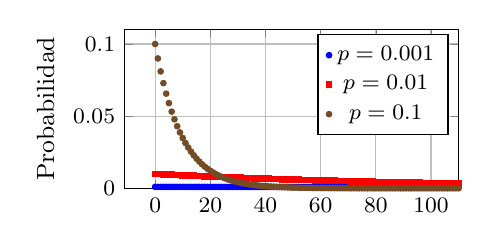
\begin{tikzpicture}
                \begin{axis}[
                    footnotesize,
                    %clip=false,
                    %domain=-2:2,
                    ymin=0,
                    %ymax={0.5},
                    xmax=110,
                    samples at={0,...,110},
                    legend entries={$p = 0.001$\\$p = 0.01$\\$p = 0.1$\\},
                    legend pos=north east,
                    legend style={font=\footnotesize},
                    ylabel=Probabilidad,
                    height=0.48\textwidth/1.618,
                    width=0.48\textwidth,
                    %xtick distance=1,
                    %axis lines=middle,
                    grid=major,
                    mark size=1pt,
                    yticklabel style={/pgf/number format/fixed},
                    %no markers,
                    ]
                    \addplot+[only marks] {(1 - 0.001)^x * 0.001};
                    \addplot+[only marks] {(1 - 0.01)^x * 0.01};
                    \addplot+[only marks] {(1 - 0.1)^x * 0.1};
                \end{axis}
            \end{tikzpicture}
            &
            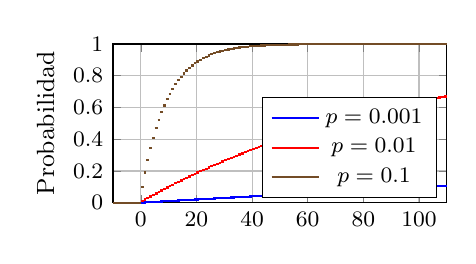
\begin{tikzpicture}
                \begin{axis}[
                    footnotesize,
                    clip=false,
                    %domain=-10:110,
                    samples at={-10,...,110},
                    ymin=0,
                    ymax=1,
                    xmin=-10,
                    xmax=110,
                    %xtick distance=1,
                    legend entries={$p = 0.001$\\$p = 0.01$\\$p = 0.1$\\},
                    legend pos=south east,
                    legend style={font=\footnotesize},
                    ylabel=Probabilidad,
                    height=0.48\textwidth/1.618,
                    width=0.48\textwidth,
                    %axis lines=middle,
                    grid=major,
                    no markers,
                    ]
                    \addplot+[thick, jump mark left] {max(0, 1 - (1 - 0.001)^(x + 1))};
                    \addplot+[thick, jump mark left] {max(0, 1 - (1 - 0.01)^(x + 1))};
                    \addplot+[thick, jump mark left] {max(0, 1 - (1 - 0.1)^(x + 1))};
                \end{axis}
            \end{tikzpicture}
        \end{tabular}
    \end{center}
    \begin{block}{¿Qué pasó?}
        \begin{itemize}
            \item $X$ ahora está expresada como una función \emph{pmf} en vez de una tabla.
        \end{itemize}
    \end{block}
\end{frame}

\begin{frame}
    \frametitle{Distribución $X \sim \text{Geométrica} \parens{p}$}
    \begin{block}{Definición}
        \begin{equation*}
        %\begin{itemize}
            \ff{x} = \prob{X = x} = \parens{1 - p}^{x-1} p , \text{ con } x \in \bparens{0, 1, 2, \ldots} .
                % \ff{x} = \prob{X = x} = p e^{- \ln{\parens{\frac{1}{1 - p}}} x} p , \text{ con } x \in \bparens{0, 1, 2, \ldots} \\
        %    \item $\ff{x} = \prob{X = x} = \parens{1 - p}^{x} p$.
        %    \item $\FF{x} = \prob{X \leq x} = 1 - \parens{1 - p}^{x + 1}$.
        %\end{itemize}
        \end{equation*}
    \end{block}
    \begin{center}
        \begin{tabular}{cc}
            \emph{pmf} ($\ff{x}$) & \emph{cdf} ($\FF{x}$) \\
            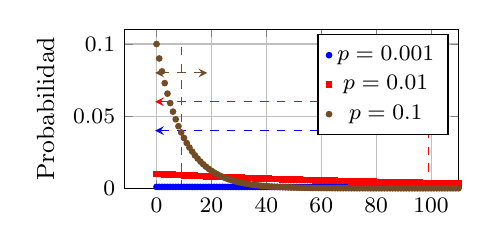
\begin{tikzpicture}
                \begin{axis}[
                    footnotesize,
                    %clip=false,
                    %domain=-2:2,
                    ymin=0,
                    %ymax={0.5},
                    xmax=110,
                    samples at={0,...,110},
                    legend entries={$p = 0.001$\\$p = 0.01$\\$p = 0.1$\\},
                    legend pos=north east,
                    legend style={font=\footnotesize},
                    ylabel=Probabilidad,
                    height=0.48\textwidth/1.618,
                    width=0.48\textwidth,
                    %xtick distance=1,
                    %axis lines=middle,
                    grid=major,
                    mark size=1pt,
                    yticklabel style={/pgf/number format/fixed},
                    %no markers,
                    ]
                    \addplot+[forget plot, dashed, no markers, stealth-] coordinates {(999 - 10 * sqrt(9990), 0.04) (100, 0.04)};
                    \addplot+[only marks] {(1 - 0.001)^x * 0.001};
                    \addplot+[forget plot, dashed, no markers] coordinates {(99, 0) (99, 0.1)};
                    \addplot+[forget plot, dashed, no markers, stealth-] coordinates {(99 - 10 * sqrt(99), 0.06) (100, 0.06)};
                    \addplot+[only marks] {(1 - 0.01)^x * 0.01};
                    \addplot+[forget plot, dashed, no markers] coordinates {(9, 0) (9, 0.1)};
                    \addplot+[forget plot, dashed, no markers, stealth-stealth] coordinates {(9 - sqrt(90), 0.08) (9 + sqrt(90), 0.08)};
                    \addplot+[only marks] {(1 - 0.1)^x * 0.1};
                \end{axis}
            \end{tikzpicture}
            &
            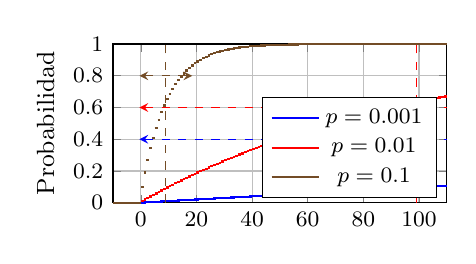
\begin{tikzpicture}
                \begin{axis}[
                    footnotesize,
                    clip=false,
                    %domain=-10:110,
                    samples at={-10,...,110},
                    ymin=0,
                    ymax=1,
                    xmin=-10,
                    xmax=110,
                    %xtick distance=1,
                    legend entries={$p = 0.001$\\$p = 0.01$\\$p = 0.1$\\},
                    legend pos=south east,
                    legend style={font=\footnotesize},
                    ylabel=Probabilidad,
                    height=0.48\textwidth/1.618,
                    width=0.48\textwidth,
                    %axis lines=middle,
                    grid=major,
                    no markers,
                    ]
                    \addplot+[forget plot, dashed, stealth-] coordinates {(999 - 10 * sqrt(9990), 0.4) (110, 0.4)};
                    \addplot+[thick, jump mark left] {max(0, 1 - (1 - 0.001)^(x + 1))};
                    \addplot+[forget plot, dashed] coordinates {(99, 0) (99, 1)};
                    \addplot+[forget plot, dashed, stealth-] coordinates {(99 - 10 * sqrt(99), 0.6) (110, 0.6)};
                    \addplot+[thick, jump mark left] {max(0, 1 - (1 - 0.01)^(x + 1))};
                    \addplot+[forget plot, dashed] coordinates {(9, 0) (9, 1)};
                    \addplot+[forget plot, dashed, stealth-stealth] coordinates {(9 - sqrt(90), 0.8) (9 + sqrt(90), 0.8)};
                    \addplot+[thick, jump mark left] {max(0, 1 - (1 - 0.1)^(x + 1))};
                \end{axis}
            \end{tikzpicture}
        \end{tabular}
    \end{center}
    \begin{block}{Propiedades}
        \begin{itemize}
            \item $\expecteddist{X \sim \text{Geométrica} \parens{p}}{X} = \mu_{X} = \frac{1}{p}$.
            \item $\variancedist{X \sim \text{Geométrica} \parens{p}}{X} = \sigma^{2}_{X} = \frac{1 - p}{p^{2}}$.

        \end{itemize}
    \end{block}
\end{frame}

\begin{frame}
    \frametitle{Ejemplo: Reunión de personas sin COVID-19}
    \begin{block}{Supuestos}
        \begin{itemize}
            \item Cada persona que llega tiene prob. $p$ de tener COVID-19.
            \item Probabilidad $p$ es independiente entre personas.
            \item $X$ personas con COVID-19 en reunión de $n$ personas.
        \end{itemize}
    \end{block}
    \begin{block}{$X$ como función \emph{pmf}}
        %\begin{itemize}
        %    \item $\ff{x} = \prob{X = x} = \frac{\binom{n}{x} p^{x} \parens{1 - p}^{n - x}}{2^{n}}$.
            % \item $\FF{x} = \prob{X \leq x} = 1 - \parens{1 - p}^{x + 1}$.
        %\end{itemize}
        \begin{equation*}
            \ff{x} = \prob{X = x} = \binom{n}{x} p^{x} \parens{1 - p}^{n - x} .
            % \item $\FF{x} = \prob{X \leq x} = 1 - \parens{1 - p}^{x + 1}$.
        \end{equation*}
    \end{block}
    \begin{center}
        \begin{tabular}{cc}
            \emph{pmf} ($\ff{x}$) con $p = 0.005$ & \emph{cdf} ($\FF{x}$) con $p = 0.005$ \\
            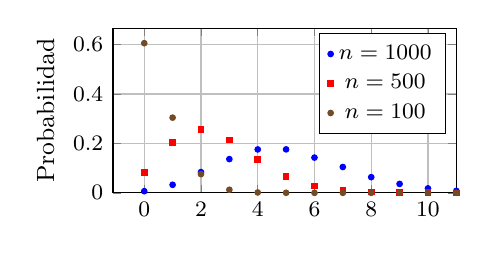
\begin{tikzpicture}
                \begin{axis}[
                    footnotesize,
                    %clip=false,
                    %domain=-2:2,
                    ymin=0,
                    %ymax={0.5},
                    xmax=11,
                    samples at={0,...,11},
                    legend entries={$n = 1000$\\$n = 500$\\$n = 100$\\},
                    legend pos=north east,
                    legend style={font=\footnotesize},
                    ylabel=Probabilidad,
                    height=0.49\textwidth/1.618,
                    width=0.49\textwidth,
                    %xtick distance=1,
                    %axis lines=middle,
                    grid=major,
                    mark size=1pt,
                    %yticklabel style={/pgf/number format/fixed},
                    %no markers,
                    ]
                    \addplot+[only marks] {factorial(1000) / factorial(1000 - x) / factorial(x) * 0.005^x * 0.995^(1000 - x)};
                    \addplot+[only marks] {factorial(500) / factorial(500 - x) / factorial(x) * 0.005^x * 0.995^(500 - x)};
                    \addplot+[only marks] {factorial(100) / factorial(100 - x) / factorial(x) * 0.005^x * 0.995^(100 - x)};
                \end{axis}
            \end{tikzpicture}
            &
            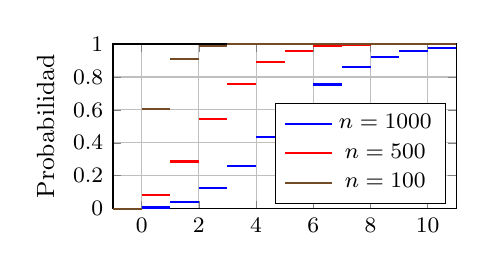
\begin{tikzpicture}
                \begin{axis}[
                    footnotesize,
                    clip=false,
                    %domain=-10:110,
                    %samples at={0,...,10},
                    ymin=0,
                    ymax=1,
                    xmin=-1,
                    xmax=11,
                    %xtick distance=1,
                    legend entries={$n = 1000$\\$n = 500$\\$n = 100$\\},
                    legend pos=south east,
                    legend style={font=\footnotesize},
                    ylabel=Probabilidad,
                    height=0.49\textwidth/1.618,
                    width=0.49\textwidth,
                    %axis lines=middle,
                    grid=major,
                    no markers,
                    ]
                    \addplot+[thick, jump mark left] coordinates {(-1, 0)
                        (0, {factorial(1000) / factorial(1000 - 0) / factorial(0) * 0.005^0 * 0.995^(1000 - 0)})
                        (1, {factorial(1000) / factorial(1000 - 1) / factorial(1) * 0.005^1 * 0.995^(1000 - 1) + factorial(1000) / factorial(1000 - 0) / factorial(0) * 0.005^0 * 0.995^(1000 - 0)})
                        (2, {factorial(1000) / factorial(1000 - 2) / factorial(2) * 0.005^2 * 0.995^(1000 - 2) + factorial(1000) / factorial(1000 - 1) / factorial(1) * 0.005^1 * 0.995^(1000 - 1) + factorial(1000) / factorial(1000 - 0) / factorial(0) * 0.005^0 * 0.995^(1000 - 0)})
                        (3, {factorial(1000) / factorial(1000 - 3) / factorial(3) * 0.005^3 * 0.995^(1000 - 3) + factorial(1000) / factorial(1000 - 2) / factorial(2) * 0.005^2 * 0.995^(1000 - 2) + factorial(1000) / factorial(1000 - 1) / factorial(1) * 0.005^1 * 0.995^(1000 - 1) + factorial(1000) / factorial(1000 - 0) / factorial(0) * 0.005^0 * 0.995^(1000 - 0)})
                        (4, {factorial(1000) / factorial(1000 - 4) / factorial(4) * 0.005^4 * 0.995^(1000 - 4) + factorial(1000) / factorial(1000 - 3) / factorial(3) * 0.005^3 * 0.995^(1000 - 3) + factorial(1000) / factorial(1000 - 2) / factorial(2) * 0.005^2 * 0.995^(1000 - 2) + factorial(1000) / factorial(1000 - 1) / factorial(1) * 0.005^1 * 0.995^(1000 - 1) + factorial(1000) / factorial(1000 - 0) / factorial(0) * 0.005^0 * 0.995^(1000 - 0)})
                        (5, {factorial(1000) / factorial(1000 - 5) / factorial(5) * 0.005^5 * 0.995^(1000 - 5) + factorial(1000) / factorial(1000 - 4) / factorial(4) * 0.005^4 * 0.995^(1000 - 4) + factorial(1000) / factorial(1000 - 3) / factorial(3) * 0.005^3 * 0.995^(1000 - 3) + factorial(1000) / factorial(1000 - 2) / factorial(2) * 0.005^2 * 0.995^(1000 - 2) + factorial(1000) / factorial(1000 - 1) / factorial(1) * 0.005^1 * 0.995^(1000 - 1) + factorial(1000) / factorial(1000 - 0) / factorial(0) * 0.005^0 * 0.995^(1000 - 0)})
                        (6, {factorial(1000) / factorial(1000 - 6) / factorial(6) * 0.005^6 * 0.995^(1000 - 6) + factorial(1000) / factorial(1000 - 5) / factorial(5) * 0.005^5 * 0.995^(1000 - 5) + factorial(1000) / factorial(1000 - 4) / factorial(4) * 0.005^4 * 0.995^(1000 - 4) + factorial(1000) / factorial(1000 - 3) / factorial(3) * 0.005^3 * 0.995^(1000 - 3) + factorial(1000) / factorial(1000 - 2) / factorial(2) * 0.005^2 * 0.995^(1000 - 2) + factorial(1000) / factorial(1000 - 1) / factorial(1) * 0.005^1 * 0.995^(1000 - 1) + factorial(1000) / factorial(1000 - 0) / factorial(0) * 0.005^0 * 0.995^(1000 - 0)})
                        (7, {factorial(1000) / factorial(1000 - 7) / factorial(7) * 0.005^7 * 0.995^(1000 - 7) + factorial(1000) / factorial(1000 - 6) / factorial(6) * 0.005^6 * 0.995^(1000 - 6) + factorial(1000) / factorial(1000 - 5) / factorial(5) * 0.005^5 * 0.995^(1000 - 5) + factorial(1000) / factorial(1000 - 4) / factorial(4) * 0.005^4 * 0.995^(1000 - 4) + factorial(1000) / factorial(1000 - 3) / factorial(3) * 0.005^3 * 0.995^(1000 - 3) + factorial(1000) / factorial(1000 - 2) / factorial(2) * 0.005^2 * 0.995^(1000 - 2) + factorial(1000) / factorial(1000 - 1) / factorial(1) * 0.005^1 * 0.995^(1000 - 1) + factorial(1000) / factorial(1000 - 0) / factorial(0) * 0.005^0 * 0.995^(1000 - 0)})
                        (8, {factorial(1000) / factorial(1000 - 8) / factorial(8) * 0.005^8 * 0.995^(1000 - 8) + factorial(1000) / factorial(1000 - 7) / factorial(7) * 0.005^7 * 0.995^(1000 - 7) + factorial(1000) / factorial(1000 - 6) / factorial(6) * 0.005^6 * 0.995^(1000 - 6) + factorial(1000) / factorial(1000 - 5) / factorial(5) * 0.005^5 * 0.995^(1000 - 5) + factorial(1000) / factorial(1000 - 4) / factorial(4) * 0.005^4 * 0.995^(1000 - 4) + factorial(1000) / factorial(1000 - 3) / factorial(3) * 0.005^3 * 0.995^(1000 - 3) + factorial(1000) / factorial(1000 - 2) / factorial(2) * 0.005^2 * 0.995^(1000 - 2) + factorial(1000) / factorial(1000 - 1) / factorial(1) * 0.005^1 * 0.995^(1000 - 1) + factorial(1000) / factorial(1000 - 0) / factorial(0) * 0.005^0 * 0.995^(1000 - 0)})
                        (9, {factorial(1000) / factorial(1000 - 9) / factorial(9) * 0.005^9 * 0.995^(1000 - 9) + factorial(1000) / factorial(1000 - 8) / factorial(8) * 0.005^8 * 0.995^(1000 - 8) + factorial(1000) / factorial(1000 - 7) / factorial(7) * 0.005^7 * 0.995^(1000 - 7) + factorial(1000) / factorial(1000 - 6) / factorial(6) * 0.005^6 * 0.995^(1000 - 6) + factorial(1000) / factorial(1000 - 5) / factorial(5) * 0.005^5 * 0.995^(1000 - 5) + factorial(1000) / factorial(1000 - 4) / factorial(4) * 0.005^4 * 0.995^(1000 - 4) + factorial(1000) / factorial(1000 - 3) / factorial(3) * 0.005^3 * 0.995^(1000 - 3) + factorial(1000) / factorial(1000 - 2) / factorial(2) * 0.005^2 * 0.995^(1000 - 2) + factorial(1000) / factorial(1000 - 1) / factorial(1) * 0.005^1 * 0.995^(1000 - 1) + factorial(1000) / factorial(1000 - 0) / factorial(0) * 0.005^0 * 0.995^(1000 - 0)})
                        (10, {factorial(1000) / factorial(1000 - 10) / factorial(10) * 0.005^10 * 0.995^(1000 - 10) + factorial(1000) / factorial(1000 - 9) / factorial(9) * 0.005^9 * 0.995^(1000 - 9) + factorial(1000) / factorial(1000 - 8) / factorial(8) * 0.005^8 * 0.995^(1000 - 8) + factorial(1000) / factorial(1000 - 7) / factorial(7) * 0.005^7 * 0.995^(1000 - 7) + factorial(1000) / factorial(1000 - 6) / factorial(6) * 0.005^6 * 0.995^(1000 - 6) + factorial(1000) / factorial(1000 - 5) / factorial(5) * 0.005^5 * 0.995^(1000 - 5) + factorial(1000) / factorial(1000 - 4) / factorial(4) * 0.005^4 * 0.995^(1000 - 4) + factorial(1000) / factorial(1000 - 3) / factorial(3) * 0.005^3 * 0.995^(1000 - 3) + factorial(1000) / factorial(1000 - 2) / factorial(2) * 0.005^2 * 0.995^(1000 - 2) + factorial(1000) / factorial(1000 - 1) / factorial(1) * 0.005^1 * 0.995^(1000 - 1) + factorial(1000) / factorial(1000 - 0) / factorial(0) * 0.005^0 * 0.995^(1000 - 0)})
                        (11, {factorial(1000) / factorial(1000 - 11) / factorial(11) * 0.005^11 * 0.995^(1000 - 11) + factorial(1000) / factorial(1000 - 10) / factorial(10) * 0.005^10 * 0.995^(1000 - 10) + factorial(1000) / factorial(1000 - 9) / factorial(9) * 0.005^9 * 0.995^(1000 - 9) + factorial(1000) / factorial(1000 - 8) / factorial(8) * 0.005^8 * 0.995^(1000 - 8) + factorial(1000) / factorial(1000 - 7) / factorial(7) * 0.005^7 * 0.995^(1000 - 7) + factorial(1000) / factorial(1000 - 6) / factorial(6) * 0.005^6 * 0.995^(1000 - 6) + factorial(1000) / factorial(1000 - 5) / factorial(5) * 0.005^5 * 0.995^(1000 - 5) + factorial(1000) / factorial(1000 - 4) / factorial(4) * 0.005^4 * 0.995^(1000 - 4) + factorial(1000) / factorial(1000 - 3) / factorial(3) * 0.005^3 * 0.995^(1000 - 3) + factorial(1000) / factorial(1000 - 2) / factorial(2) * 0.005^2 * 0.995^(1000 - 2) + factorial(1000) / factorial(1000 - 1) / factorial(1) * 0.005^1 * 0.995^(1000 - 1) + factorial(1000) / factorial(1000 - 0) / factorial(0) * 0.005^0 * 0.995^(1000 - 0)})};
                    \addplot+[thick, jump mark left] coordinates {(-1, 0)
                        (0, {factorial(500) / factorial(500 - 0) / factorial(0) * 0.005^0 * 0.995^(500 - 0)})
                        (1, {factorial(500) / factorial(500 - 1) / factorial(1) * 0.005^1 * 0.995^(500 - 1) + factorial(500) / factorial(500 - 0) / factorial(0) * 0.005^0 * 0.995^(500 - 0)})
                        (2, {factorial(500) / factorial(500 - 2) / factorial(2) * 0.005^2 * 0.995^(500 - 2) + factorial(500) / factorial(500 - 1) / factorial(1) * 0.005^1 * 0.995^(500 - 1) + factorial(500) / factorial(500 - 0) / factorial(0) * 0.005^0 * 0.995^(500 - 0)})
                        (3, {factorial(500) / factorial(500 - 3) / factorial(3) * 0.005^3 * 0.995^(500 - 3) + factorial(500) / factorial(500 - 2) / factorial(2) * 0.005^2 * 0.995^(500 - 2) + factorial(500) / factorial(500 - 1) / factorial(1) * 0.005^1 * 0.995^(500 - 1) + factorial(500) / factorial(500 - 0) / factorial(0) * 0.005^0 * 0.995^(500 - 0)})
                        (4, {factorial(500) / factorial(500 - 4) / factorial(4) * 0.005^4 * 0.995^(500 - 4) + factorial(500) / factorial(500 - 3) / factorial(3) * 0.005^3 * 0.995^(500 - 3) + factorial(500) / factorial(500 - 2) / factorial(2) * 0.005^2 * 0.995^(500 - 2) + factorial(500) / factorial(500 - 1) / factorial(1) * 0.005^1 * 0.995^(500 - 1) + factorial(500) / factorial(500 - 0) / factorial(0) * 0.005^0 * 0.995^(500 - 0)})
                        (5, {factorial(500) / factorial(500 - 5) / factorial(5) * 0.005^5 * 0.995^(500 - 5) + factorial(500) / factorial(500 - 4) / factorial(4) * 0.005^4 * 0.995^(500 - 4) + factorial(500) / factorial(500 - 3) / factorial(3) * 0.005^3 * 0.995^(500 - 3) + factorial(500) / factorial(500 - 2) / factorial(2) * 0.005^2 * 0.995^(500 - 2) + factorial(500) / factorial(500 - 1) / factorial(1) * 0.005^1 * 0.995^(500 - 1) + factorial(500) / factorial(500 - 0) / factorial(0) * 0.005^0 * 0.995^(500 - 0)})
                        (6, {factorial(500) / factorial(500 - 6) / factorial(6) * 0.005^6 * 0.995^(500 - 6) + factorial(500) / factorial(500 - 5) / factorial(5) * 0.005^5 * 0.995^(500 - 5) + factorial(500) / factorial(500 - 4) / factorial(4) * 0.005^4 * 0.995^(500 - 4) + factorial(500) / factorial(500 - 3) / factorial(3) * 0.005^3 * 0.995^(500 - 3) + factorial(500) / factorial(500 - 2) / factorial(2) * 0.005^2 * 0.995^(500 - 2) + factorial(500) / factorial(500 - 1) / factorial(1) * 0.005^1 * 0.995^(500 - 1) + factorial(500) / factorial(500 - 0) / factorial(0) * 0.005^0 * 0.995^(500 - 0)})
                        (7, {factorial(500) / factorial(500 - 7) / factorial(7) * 0.005^7 * 0.995^(500 - 7) + factorial(500) / factorial(500 - 6) / factorial(6) * 0.005^6 * 0.995^(500 - 6) + factorial(500) / factorial(500 - 5) / factorial(5) * 0.005^5 * 0.995^(500 - 5) + factorial(500) / factorial(500 - 4) / factorial(4) * 0.005^4 * 0.995^(500 - 4) + factorial(500) / factorial(500 - 3) / factorial(3) * 0.005^3 * 0.995^(500 - 3) + factorial(500) / factorial(500 - 2) / factorial(2) * 0.005^2 * 0.995^(500 - 2) + factorial(500) / factorial(500 - 1) / factorial(1) * 0.005^1 * 0.995^(500 - 1) + factorial(500) / factorial(500 - 0) / factorial(0) * 0.005^0 * 0.995^(500 - 0)})
                        (8, {factorial(500) / factorial(500 - 8) / factorial(8) * 0.005^8 * 0.995^(500 - 8) + factorial(500) / factorial(500 - 7) / factorial(7) * 0.005^7 * 0.995^(500 - 7) + factorial(500) / factorial(500 - 6) / factorial(6) * 0.005^6 * 0.995^(500 - 6) + factorial(500) / factorial(500 - 5) / factorial(5) * 0.005^5 * 0.995^(500 - 5) + factorial(500) / factorial(500 - 4) / factorial(4) * 0.005^4 * 0.995^(500 - 4) + factorial(500) / factorial(500 - 3) / factorial(3) * 0.005^3 * 0.995^(500 - 3) + factorial(500) / factorial(500 - 2) / factorial(2) * 0.005^2 * 0.995^(500 - 2) + factorial(500) / factorial(500 - 1) / factorial(1) * 0.005^1 * 0.995^(500 - 1) + factorial(500) / factorial(500 - 0) / factorial(0) * 0.005^0 * 0.995^(500 - 0)})
                        (9, {factorial(500) / factorial(500 - 9) / factorial(9) * 0.005^9 * 0.995^(500 - 9) + factorial(500) / factorial(500 - 8) / factorial(8) * 0.005^8 * 0.995^(500 - 8) + factorial(500) / factorial(500 - 7) / factorial(7) * 0.005^7 * 0.995^(500 - 7) + factorial(500) / factorial(500 - 6) / factorial(6) * 0.005^6 * 0.995^(500 - 6) + factorial(500) / factorial(500 - 5) / factorial(5) * 0.005^5 * 0.995^(500 - 5) + factorial(500) / factorial(500 - 4) / factorial(4) * 0.005^4 * 0.995^(500 - 4) + factorial(500) / factorial(500 - 3) / factorial(3) * 0.005^3 * 0.995^(500 - 3) + factorial(500) / factorial(500 - 2) / factorial(2) * 0.005^2 * 0.995^(500 - 2) + factorial(500) / factorial(500 - 1) / factorial(1) * 0.005^1 * 0.995^(500 - 1) + factorial(500) / factorial(500 - 0) / factorial(0) * 0.005^0 * 0.995^(500 - 0)})
                        (10, {factorial(500) / factorial(500 - 10) / factorial(10) * 0.005^10 * 0.995^(500 - 10) + factorial(500) / factorial(500 - 9) / factorial(9) * 0.005^9 * 0.995^(500 - 9) + factorial(500) / factorial(500 - 8) / factorial(8) * 0.005^8 * 0.995^(500 - 8) + factorial(500) / factorial(500 - 7) / factorial(7) * 0.005^7 * 0.995^(500 - 7) + factorial(500) / factorial(500 - 6) / factorial(6) * 0.005^6 * 0.995^(500 - 6) + factorial(500) / factorial(500 - 5) / factorial(5) * 0.005^5 * 0.995^(500 - 5) + factorial(500) / factorial(500 - 4) / factorial(4) * 0.005^4 * 0.995^(500 - 4) + factorial(500) / factorial(500 - 3) / factorial(3) * 0.005^3 * 0.995^(500 - 3) + factorial(500) / factorial(500 - 2) / factorial(2) * 0.005^2 * 0.995^(500 - 2) + factorial(500) / factorial(500 - 1) / factorial(1) * 0.005^1 * 0.995^(500 - 1) + factorial(500) / factorial(500 - 0) / factorial(0) * 0.005^0 * 0.995^(500 - 0)})
                        (11, {factorial(500) / factorial(500 - 11) / factorial(11) * 0.005^11 * 0.995^(500 - 11) + factorial(500) / factorial(500 - 10) / factorial(10) * 0.005^10 * 0.995^(500 - 10) + factorial(500) / factorial(500 - 9) / factorial(9) * 0.005^9 * 0.995^(500 - 9) + factorial(500) / factorial(500 - 8) / factorial(8) * 0.005^8 * 0.995^(500 - 8) + factorial(500) / factorial(500 - 7) / factorial(7) * 0.005^7 * 0.995^(500 - 7) + factorial(500) / factorial(500 - 6) / factorial(6) * 0.005^6 * 0.995^(500 - 6) + factorial(500) / factorial(500 - 5) / factorial(5) * 0.005^5 * 0.995^(500 - 5) + factorial(500) / factorial(500 - 4) / factorial(4) * 0.005^4 * 0.995^(500 - 4) + factorial(500) / factorial(500 - 3) / factorial(3) * 0.005^3 * 0.995^(500 - 3) + factorial(500) / factorial(500 - 2) / factorial(2) * 0.005^2 * 0.995^(500 - 2) + factorial(500) / factorial(500 - 1) / factorial(1) * 0.005^1 * 0.995^(500 - 1) + factorial(500) / factorial(500 - 0) / factorial(0) * 0.005^0 * 0.995^(500 - 0)})};
                    \addplot+[thick, jump mark left] coordinates {(-1, 0)
                        (0, {factorial(100) / factorial(100 - 0) / factorial(0) * 0.005^0 * 0.995^(100 - 0)})
                        (1, {factorial(100) / factorial(100 - 1) / factorial(1) * 0.005^1 * 0.995^(100 - 1) + factorial(100) / factorial(100 - 0) / factorial(0) * 0.005^0 * 0.995^(100 - 0)})
                        (2, {factorial(100) / factorial(100 - 2) / factorial(2) * 0.005^2 * 0.995^(100 - 2) + factorial(100) / factorial(100 - 1) / factorial(1) * 0.005^1 * 0.995^(100 - 1) + factorial(100) / factorial(100 - 0) / factorial(0) * 0.005^0 * 0.995^(100 - 0)})
                        (3, {factorial(100) / factorial(100 - 3) / factorial(3) * 0.005^3 * 0.995^(100 - 3) + factorial(100) / factorial(100 - 2) / factorial(2) * 0.005^2 * 0.995^(100 - 2) + factorial(100) / factorial(100 - 1) / factorial(1) * 0.005^1 * 0.995^(100 - 1) + factorial(100) / factorial(100 - 0) / factorial(0) * 0.005^0 * 0.995^(100 - 0)})
                        (4, {factorial(100) / factorial(100 - 4) / factorial(4) * 0.005^4 * 0.995^(100 - 4) + factorial(100) / factorial(100 - 3) / factorial(3) * 0.005^3 * 0.995^(100 - 3) + factorial(100) / factorial(100 - 2) / factorial(2) * 0.005^2 * 0.995^(100 - 2) + factorial(100) / factorial(100 - 1) / factorial(1) * 0.005^1 * 0.995^(100 - 1) + factorial(100) / factorial(100 - 0) / factorial(0) * 0.005^0 * 0.995^(100 - 0)})
                        (5, {factorial(100) / factorial(100 - 5) / factorial(5) * 0.005^5 * 0.995^(100 - 5) + factorial(100) / factorial(100 - 4) / factorial(4) * 0.005^4 * 0.995^(100 - 4) + factorial(100) / factorial(100 - 3) / factorial(3) * 0.005^3 * 0.995^(100 - 3) + factorial(100) / factorial(100 - 2) / factorial(2) * 0.005^2 * 0.995^(100 - 2) + factorial(100) / factorial(100 - 1) / factorial(1) * 0.005^1 * 0.995^(100 - 1) + factorial(100) / factorial(100 - 0) / factorial(0) * 0.005^0 * 0.995^(100 - 0)})
                        (6, {factorial(100) / factorial(100 - 6) / factorial(6) * 0.005^6 * 0.995^(100 - 6) + factorial(100) / factorial(100 - 5) / factorial(5) * 0.005^5 * 0.995^(100 - 5) + factorial(100) / factorial(100 - 4) / factorial(4) * 0.005^4 * 0.995^(100 - 4) + factorial(100) / factorial(100 - 3) / factorial(3) * 0.005^3 * 0.995^(100 - 3) + factorial(100) / factorial(100 - 2) / factorial(2) * 0.005^2 * 0.995^(100 - 2) + factorial(100) / factorial(100 - 1) / factorial(1) * 0.005^1 * 0.995^(100 - 1) + factorial(100) / factorial(100 - 0) / factorial(0) * 0.005^0 * 0.995^(100 - 0)})
                        (7, {factorial(100) / factorial(100 - 7) / factorial(7) * 0.005^7 * 0.995^(100 - 7) + factorial(100) / factorial(100 - 6) / factorial(6) * 0.005^6 * 0.995^(100 - 6) + factorial(100) / factorial(100 - 5) / factorial(5) * 0.005^5 * 0.995^(100 - 5) + factorial(100) / factorial(100 - 4) / factorial(4) * 0.005^4 * 0.995^(100 - 4) + factorial(100) / factorial(100 - 3) / factorial(3) * 0.005^3 * 0.995^(100 - 3) + factorial(100) / factorial(100 - 2) / factorial(2) * 0.005^2 * 0.995^(100 - 2) + factorial(100) / factorial(100 - 1) / factorial(1) * 0.005^1 * 0.995^(100 - 1) + factorial(100) / factorial(100 - 0) / factorial(0) * 0.005^0 * 0.995^(100 - 0)})
                        (8, {factorial(100) / factorial(100 - 8) / factorial(8) * 0.005^8 * 0.995^(100 - 8) + factorial(100) / factorial(100 - 7) / factorial(7) * 0.005^7 * 0.995^(100 - 7) + factorial(100) / factorial(100 - 6) / factorial(6) * 0.005^6 * 0.995^(100 - 6) + factorial(100) / factorial(100 - 5) / factorial(5) * 0.005^5 * 0.995^(100 - 5) + factorial(100) / factorial(100 - 4) / factorial(4) * 0.005^4 * 0.995^(100 - 4) + factorial(100) / factorial(100 - 3) / factorial(3) * 0.005^3 * 0.995^(100 - 3) + factorial(100) / factorial(100 - 2) / factorial(2) * 0.005^2 * 0.995^(100 - 2) + factorial(100) / factorial(100 - 1) / factorial(1) * 0.005^1 * 0.995^(100 - 1) + factorial(100) / factorial(100 - 0) / factorial(0) * 0.005^0 * 0.995^(100 - 0)})
                        (9, {factorial(100) / factorial(100 - 9) / factorial(9) * 0.005^9 * 0.995^(100 - 9) + factorial(100) / factorial(100 - 8) / factorial(8) * 0.005^8 * 0.995^(100 - 8) + factorial(100) / factorial(100 - 7) / factorial(7) * 0.005^7 * 0.995^(100 - 7) + factorial(100) / factorial(100 - 6) / factorial(6) * 0.005^6 * 0.995^(100 - 6) + factorial(100) / factorial(100 - 5) / factorial(5) * 0.005^5 * 0.995^(100 - 5) + factorial(100) / factorial(100 - 4) / factorial(4) * 0.005^4 * 0.995^(100 - 4) + factorial(100) / factorial(100 - 3) / factorial(3) * 0.005^3 * 0.995^(100 - 3) + factorial(100) / factorial(100 - 2) / factorial(2) * 0.005^2 * 0.995^(100 - 2) + factorial(100) / factorial(100 - 1) / factorial(1) * 0.005^1 * 0.995^(100 - 1) + factorial(100) / factorial(100 - 0) / factorial(0) * 0.005^0 * 0.995^(100 - 0)})
                        (10, {factorial(100) / factorial(100 - 10) / factorial(10) * 0.005^10 * 0.995^(100 - 10) + factorial(100) / factorial(100 - 9) / factorial(9) * 0.005^9 * 0.995^(100 - 9) + factorial(100) / factorial(100 - 8) / factorial(8) * 0.005^8 * 0.995^(100 - 8) + factorial(100) / factorial(100 - 7) / factorial(7) * 0.005^7 * 0.995^(100 - 7) + factorial(100) / factorial(100 - 6) / factorial(6) * 0.005^6 * 0.995^(100 - 6) + factorial(100) / factorial(100 - 5) / factorial(5) * 0.005^5 * 0.995^(100 - 5) + factorial(100) / factorial(100 - 4) / factorial(4) * 0.005^4 * 0.995^(100 - 4) + factorial(100) / factorial(100 - 3) / factorial(3) * 0.005^3 * 0.995^(100 - 3) + factorial(100) / factorial(100 - 2) / factorial(2) * 0.005^2 * 0.995^(100 - 2) + factorial(100) / factorial(100 - 1) / factorial(1) * 0.005^1 * 0.995^(100 - 1) + factorial(100) / factorial(100 - 0) / factorial(0) * 0.005^0 * 0.995^(100 - 0)})
                        (11, {factorial(100) / factorial(100 - 11) / factorial(11) * 0.005^11 * 0.995^(100 - 11) + factorial(100) / factorial(100 - 10) / factorial(10) * 0.005^10 * 0.995^(100 - 10) + factorial(100) / factorial(100 - 9) / factorial(9) * 0.005^9 * 0.995^(100 - 9) + factorial(100) / factorial(100 - 8) / factorial(8) * 0.005^8 * 0.995^(100 - 8) + factorial(100) / factorial(100 - 7) / factorial(7) * 0.005^7 * 0.995^(100 - 7) + factorial(100) / factorial(100 - 6) / factorial(6) * 0.005^6 * 0.995^(100 - 6) + factorial(100) / factorial(100 - 5) / factorial(5) * 0.005^5 * 0.995^(100 - 5) + factorial(100) / factorial(100 - 4) / factorial(4) * 0.005^4 * 0.995^(100 - 4) + factorial(100) / factorial(100 - 3) / factorial(3) * 0.005^3 * 0.995^(100 - 3) + factorial(100) / factorial(100 - 2) / factorial(2) * 0.005^2 * 0.995^(100 - 2) + factorial(100) / factorial(100 - 1) / factorial(1) * 0.005^1 * 0.995^(100 - 1) + factorial(100) / factorial(100 - 0) / factorial(0) * 0.005^0 * 0.995^(100 - 0)})};
                \end{axis}
            \end{tikzpicture}
        \end{tabular}
    \end{center}
\end{frame}

\begin{frame}
    \frametitle{Distribución $X \sim \text{Binomial} \parens{n, p} = \binomial{n}{p}$}
    \begin{block}{Definición}
            \begin{equation*}
                \ff{x} = \binom{n}{x} p^{x} \parens{1 - p}^{n - x} , \text{ con } x \in \bparens{0, 1, \ldots n} .
            \end{equation*}
    \end{block}
    %\begin{block}{Ejemplos}
    %    \begin{itemize}
    %        \item Cantidad de caras en $n$ lanzamientos de una moneda.
    %        \item Cantidad de personas con COVID-19 en reunión de $n$ personas.
    %    \end{itemize}
    %\end{block}
    \begin{center}
        \begin{tabular}{cc}
            \emph{pmf} ($\ff{x}$) & \emph{cdf} ($\FF{x}$) \\
            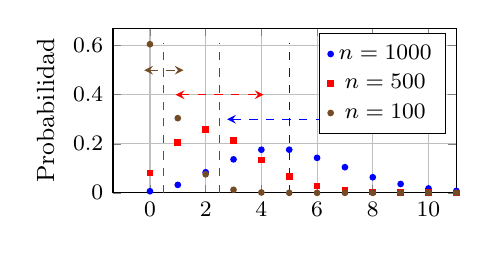
\begin{tikzpicture}
                \begin{axis}[
                    footnotesize,
                    %clip=false,
                    %domain=-2:2,
                    ymin=0,
                    %ymax={0.5},
                    xmax=11,
                    samples at={0,...,11},
                    legend entries={$n = 1000$\\$n = 500$\\$n = 100$\\},
                    legend pos=north east,
                    legend style={font=\footnotesize},
                    ylabel=Probabilidad,
                    height=0.49\textwidth/1.618,
                    width=0.49\textwidth,
                    %xtick distance=1,
                    %axis lines=middle,
                    grid=major,
                    mark size=1pt,
                    %yticklabel style={/pgf/number format/fixed},
                    %no markers,
                    ]
                    \addplot+[forget plot, dashed, no markers] coordinates {(1000 * 0.005, 0) (1000 * 0.005, 0.61)};%0.995^1000)};
                    \addplot+[forget plot, dashed, no markers, stealth-stealth] coordinates {(1000 * 0.005 - sqrt(1000 * 0.005 * 0.995), 0.3) (1000 * 0.005 + sqrt(1000 * 0.005 * 0.995), 0.3)};
                    \addplot+[only marks] {factorial(1000) / factorial(1000 - x) / factorial(x) * 0.005^x * 0.995^(1000 - x)};
                    \addplot+[forget plot, dashed, no markers] coordinates {(500 * 0.005, 0) (500 * 0.005, 0.61)};%0.995^1000)};
                    \addplot+[forget plot, dashed, no markers, stealth-stealth] coordinates {(500 * 0.005 - sqrt(500 * 0.005 * 0.995), 0.4) (500 * 0.005 + sqrt(500 * 0.005 * 0.995), 0.4)};
                    \addplot+[only marks] {factorial(500) / factorial(500 - x) / factorial(x) * 0.005^x * 0.995^(500 - x)};
                    \addplot+[forget plot, dashed, no markers] coordinates {(100 * 0.005, 0) (100 * 0.005, 0.61)};%0.995^1000)};
                    \addplot+[forget plot, dashed, no markers, stealth-stealth] coordinates {(100 * 0.005 - sqrt(100 * 0.005 * 0.995), 0.5) (100 * 0.005 + sqrt(100 * 0.005 * 0.995), 0.5)};
                    \addplot+[only marks] {factorial(100) / factorial(100 - x) / factorial(x) * 0.005^x * 0.995^(100 - x)};
                \end{axis}
            \end{tikzpicture}
            &
            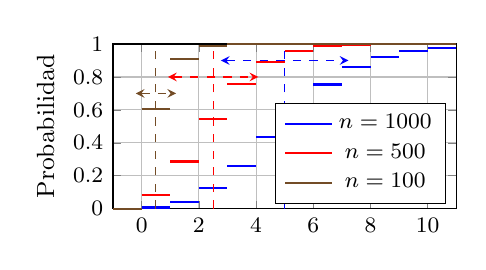
\begin{tikzpicture}
                \begin{axis}[
                    footnotesize,
                    clip=false,
                    %domain=-10:110,
                    %samples at={0,...,10},
                    ymin=0,
                    ymax=1,
                    xmin=-1,
                    xmax=11,
                    %xtick distance=1,
                    legend entries={$n = 1000$\\$n = 500$\\$n = 100$\\},
                    legend pos=south east,
                    legend style={font=\footnotesize},
                    ylabel=Probabilidad,
                    height=0.49\textwidth/1.618,
                    width=0.49\textwidth,
                    %axis lines=middle,
                    grid=major,
                    no markers,
                    ]
                    \addplot+[forget plot, dashed, no markers] coordinates {(1000 * 0.005, 0) (1000 * 0.005, 1)};
                    \addplot+[forget plot, dashed, no markers, stealth-stealth] coordinates {(1000 * 0.005 - sqrt(1000 * 0.005 * 0.995), 0.9) (1000 * 0.005 + sqrt(1000 * 0.005 * 0.995), 0.9)};
                    \addplot+[thick, jump mark left] coordinates {(-1, 0)
                        (0, {factorial(1000) / factorial(1000 - 0) / factorial(0) * 0.005^0 * 0.995^(1000 - 0)})
                        (1, {factorial(1000) / factorial(1000 - 1) / factorial(1) * 0.005^1 * 0.995^(1000 - 1) + factorial(1000) / factorial(1000 - 0) / factorial(0) * 0.005^0 * 0.995^(1000 - 0)})
                        (2, {factorial(1000) / factorial(1000 - 2) / factorial(2) * 0.005^2 * 0.995^(1000 - 2) + factorial(1000) / factorial(1000 - 1) / factorial(1) * 0.005^1 * 0.995^(1000 - 1) + factorial(1000) / factorial(1000 - 0) / factorial(0) * 0.005^0 * 0.995^(1000 - 0)})
                        (3, {factorial(1000) / factorial(1000 - 3) / factorial(3) * 0.005^3 * 0.995^(1000 - 3) + factorial(1000) / factorial(1000 - 2) / factorial(2) * 0.005^2 * 0.995^(1000 - 2) + factorial(1000) / factorial(1000 - 1) / factorial(1) * 0.005^1 * 0.995^(1000 - 1) + factorial(1000) / factorial(1000 - 0) / factorial(0) * 0.005^0 * 0.995^(1000 - 0)})
                        (4, {factorial(1000) / factorial(1000 - 4) / factorial(4) * 0.005^4 * 0.995^(1000 - 4) + factorial(1000) / factorial(1000 - 3) / factorial(3) * 0.005^3 * 0.995^(1000 - 3) + factorial(1000) / factorial(1000 - 2) / factorial(2) * 0.005^2 * 0.995^(1000 - 2) + factorial(1000) / factorial(1000 - 1) / factorial(1) * 0.005^1 * 0.995^(1000 - 1) + factorial(1000) / factorial(1000 - 0) / factorial(0) * 0.005^0 * 0.995^(1000 - 0)})
                        (5, {factorial(1000) / factorial(1000 - 5) / factorial(5) * 0.005^5 * 0.995^(1000 - 5) + factorial(1000) / factorial(1000 - 4) / factorial(4) * 0.005^4 * 0.995^(1000 - 4) + factorial(1000) / factorial(1000 - 3) / factorial(3) * 0.005^3 * 0.995^(1000 - 3) + factorial(1000) / factorial(1000 - 2) / factorial(2) * 0.005^2 * 0.995^(1000 - 2) + factorial(1000) / factorial(1000 - 1) / factorial(1) * 0.005^1 * 0.995^(1000 - 1) + factorial(1000) / factorial(1000 - 0) / factorial(0) * 0.005^0 * 0.995^(1000 - 0)})
                        (6, {factorial(1000) / factorial(1000 - 6) / factorial(6) * 0.005^6 * 0.995^(1000 - 6) + factorial(1000) / factorial(1000 - 5) / factorial(5) * 0.005^5 * 0.995^(1000 - 5) + factorial(1000) / factorial(1000 - 4) / factorial(4) * 0.005^4 * 0.995^(1000 - 4) + factorial(1000) / factorial(1000 - 3) / factorial(3) * 0.005^3 * 0.995^(1000 - 3) + factorial(1000) / factorial(1000 - 2) / factorial(2) * 0.005^2 * 0.995^(1000 - 2) + factorial(1000) / factorial(1000 - 1) / factorial(1) * 0.005^1 * 0.995^(1000 - 1) + factorial(1000) / factorial(1000 - 0) / factorial(0) * 0.005^0 * 0.995^(1000 - 0)})
                        (7, {factorial(1000) / factorial(1000 - 7) / factorial(7) * 0.005^7 * 0.995^(1000 - 7) + factorial(1000) / factorial(1000 - 6) / factorial(6) * 0.005^6 * 0.995^(1000 - 6) + factorial(1000) / factorial(1000 - 5) / factorial(5) * 0.005^5 * 0.995^(1000 - 5) + factorial(1000) / factorial(1000 - 4) / factorial(4) * 0.005^4 * 0.995^(1000 - 4) + factorial(1000) / factorial(1000 - 3) / factorial(3) * 0.005^3 * 0.995^(1000 - 3) + factorial(1000) / factorial(1000 - 2) / factorial(2) * 0.005^2 * 0.995^(1000 - 2) + factorial(1000) / factorial(1000 - 1) / factorial(1) * 0.005^1 * 0.995^(1000 - 1) + factorial(1000) / factorial(1000 - 0) / factorial(0) * 0.005^0 * 0.995^(1000 - 0)})
                        (8, {factorial(1000) / factorial(1000 - 8) / factorial(8) * 0.005^8 * 0.995^(1000 - 8) + factorial(1000) / factorial(1000 - 7) / factorial(7) * 0.005^7 * 0.995^(1000 - 7) + factorial(1000) / factorial(1000 - 6) / factorial(6) * 0.005^6 * 0.995^(1000 - 6) + factorial(1000) / factorial(1000 - 5) / factorial(5) * 0.005^5 * 0.995^(1000 - 5) + factorial(1000) / factorial(1000 - 4) / factorial(4) * 0.005^4 * 0.995^(1000 - 4) + factorial(1000) / factorial(1000 - 3) / factorial(3) * 0.005^3 * 0.995^(1000 - 3) + factorial(1000) / factorial(1000 - 2) / factorial(2) * 0.005^2 * 0.995^(1000 - 2) + factorial(1000) / factorial(1000 - 1) / factorial(1) * 0.005^1 * 0.995^(1000 - 1) + factorial(1000) / factorial(1000 - 0) / factorial(0) * 0.005^0 * 0.995^(1000 - 0)})
                        (9, {factorial(1000) / factorial(1000 - 9) / factorial(9) * 0.005^9 * 0.995^(1000 - 9) + factorial(1000) / factorial(1000 - 8) / factorial(8) * 0.005^8 * 0.995^(1000 - 8) + factorial(1000) / factorial(1000 - 7) / factorial(7) * 0.005^7 * 0.995^(1000 - 7) + factorial(1000) / factorial(1000 - 6) / factorial(6) * 0.005^6 * 0.995^(1000 - 6) + factorial(1000) / factorial(1000 - 5) / factorial(5) * 0.005^5 * 0.995^(1000 - 5) + factorial(1000) / factorial(1000 - 4) / factorial(4) * 0.005^4 * 0.995^(1000 - 4) + factorial(1000) / factorial(1000 - 3) / factorial(3) * 0.005^3 * 0.995^(1000 - 3) + factorial(1000) / factorial(1000 - 2) / factorial(2) * 0.005^2 * 0.995^(1000 - 2) + factorial(1000) / factorial(1000 - 1) / factorial(1) * 0.005^1 * 0.995^(1000 - 1) + factorial(1000) / factorial(1000 - 0) / factorial(0) * 0.005^0 * 0.995^(1000 - 0)})
                        (10, {factorial(1000) / factorial(1000 - 10) / factorial(10) * 0.005^10 * 0.995^(1000 - 10) + factorial(1000) / factorial(1000 - 9) / factorial(9) * 0.005^9 * 0.995^(1000 - 9) + factorial(1000) / factorial(1000 - 8) / factorial(8) * 0.005^8 * 0.995^(1000 - 8) + factorial(1000) / factorial(1000 - 7) / factorial(7) * 0.005^7 * 0.995^(1000 - 7) + factorial(1000) / factorial(1000 - 6) / factorial(6) * 0.005^6 * 0.995^(1000 - 6) + factorial(1000) / factorial(1000 - 5) / factorial(5) * 0.005^5 * 0.995^(1000 - 5) + factorial(1000) / factorial(1000 - 4) / factorial(4) * 0.005^4 * 0.995^(1000 - 4) + factorial(1000) / factorial(1000 - 3) / factorial(3) * 0.005^3 * 0.995^(1000 - 3) + factorial(1000) / factorial(1000 - 2) / factorial(2) * 0.005^2 * 0.995^(1000 - 2) + factorial(1000) / factorial(1000 - 1) / factorial(1) * 0.005^1 * 0.995^(1000 - 1) + factorial(1000) / factorial(1000 - 0) / factorial(0) * 0.005^0 * 0.995^(1000 - 0)})
                        (11, {factorial(1000) / factorial(1000 - 11) / factorial(11) * 0.005^11 * 0.995^(1000 - 11) + factorial(1000) / factorial(1000 - 10) / factorial(10) * 0.005^10 * 0.995^(1000 - 10) + factorial(1000) / factorial(1000 - 9) / factorial(9) * 0.005^9 * 0.995^(1000 - 9) + factorial(1000) / factorial(1000 - 8) / factorial(8) * 0.005^8 * 0.995^(1000 - 8) + factorial(1000) / factorial(1000 - 7) / factorial(7) * 0.005^7 * 0.995^(1000 - 7) + factorial(1000) / factorial(1000 - 6) / factorial(6) * 0.005^6 * 0.995^(1000 - 6) + factorial(1000) / factorial(1000 - 5) / factorial(5) * 0.005^5 * 0.995^(1000 - 5) + factorial(1000) / factorial(1000 - 4) / factorial(4) * 0.005^4 * 0.995^(1000 - 4) + factorial(1000) / factorial(1000 - 3) / factorial(3) * 0.005^3 * 0.995^(1000 - 3) + factorial(1000) / factorial(1000 - 2) / factorial(2) * 0.005^2 * 0.995^(1000 - 2) + factorial(1000) / factorial(1000 - 1) / factorial(1) * 0.005^1 * 0.995^(1000 - 1) + factorial(1000) / factorial(1000 - 0) / factorial(0) * 0.005^0 * 0.995^(1000 - 0)})};
                    \addplot+[forget plot, dashed, no markers] coordinates {(500 * 0.005, 0) (500 * 0.005, 1)};
                    \addplot+[forget plot, dashed, no markers, stealth-stealth] coordinates {(500 * 0.005 - sqrt(500 * 0.005 * 0.995), 0.8) (500 * 0.005 + sqrt(500 * 0.005 * 0.995), 0.8)};
                    \addplot+[thick, jump mark left] coordinates {(-1, 0)
                        (0, {factorial(500) / factorial(500 - 0) / factorial(0) * 0.005^0 * 0.995^(500 - 0)})
                        (1, {factorial(500) / factorial(500 - 1) / factorial(1) * 0.005^1 * 0.995^(500 - 1) + factorial(500) / factorial(500 - 0) / factorial(0) * 0.005^0 * 0.995^(500 - 0)})
                        (2, {factorial(500) / factorial(500 - 2) / factorial(2) * 0.005^2 * 0.995^(500 - 2) + factorial(500) / factorial(500 - 1) / factorial(1) * 0.005^1 * 0.995^(500 - 1) + factorial(500) / factorial(500 - 0) / factorial(0) * 0.005^0 * 0.995^(500 - 0)})
                        (3, {factorial(500) / factorial(500 - 3) / factorial(3) * 0.005^3 * 0.995^(500 - 3) + factorial(500) / factorial(500 - 2) / factorial(2) * 0.005^2 * 0.995^(500 - 2) + factorial(500) / factorial(500 - 1) / factorial(1) * 0.005^1 * 0.995^(500 - 1) + factorial(500) / factorial(500 - 0) / factorial(0) * 0.005^0 * 0.995^(500 - 0)})
                        (4, {factorial(500) / factorial(500 - 4) / factorial(4) * 0.005^4 * 0.995^(500 - 4) + factorial(500) / factorial(500 - 3) / factorial(3) * 0.005^3 * 0.995^(500 - 3) + factorial(500) / factorial(500 - 2) / factorial(2) * 0.005^2 * 0.995^(500 - 2) + factorial(500) / factorial(500 - 1) / factorial(1) * 0.005^1 * 0.995^(500 - 1) + factorial(500) / factorial(500 - 0) / factorial(0) * 0.005^0 * 0.995^(500 - 0)})
                        (5, {factorial(500) / factorial(500 - 5) / factorial(5) * 0.005^5 * 0.995^(500 - 5) + factorial(500) / factorial(500 - 4) / factorial(4) * 0.005^4 * 0.995^(500 - 4) + factorial(500) / factorial(500 - 3) / factorial(3) * 0.005^3 * 0.995^(500 - 3) + factorial(500) / factorial(500 - 2) / factorial(2) * 0.005^2 * 0.995^(500 - 2) + factorial(500) / factorial(500 - 1) / factorial(1) * 0.005^1 * 0.995^(500 - 1) + factorial(500) / factorial(500 - 0) / factorial(0) * 0.005^0 * 0.995^(500 - 0)})
                        (6, {factorial(500) / factorial(500 - 6) / factorial(6) * 0.005^6 * 0.995^(500 - 6) + factorial(500) / factorial(500 - 5) / factorial(5) * 0.005^5 * 0.995^(500 - 5) + factorial(500) / factorial(500 - 4) / factorial(4) * 0.005^4 * 0.995^(500 - 4) + factorial(500) / factorial(500 - 3) / factorial(3) * 0.005^3 * 0.995^(500 - 3) + factorial(500) / factorial(500 - 2) / factorial(2) * 0.005^2 * 0.995^(500 - 2) + factorial(500) / factorial(500 - 1) / factorial(1) * 0.005^1 * 0.995^(500 - 1) + factorial(500) / factorial(500 - 0) / factorial(0) * 0.005^0 * 0.995^(500 - 0)})
                        (7, {factorial(500) / factorial(500 - 7) / factorial(7) * 0.005^7 * 0.995^(500 - 7) + factorial(500) / factorial(500 - 6) / factorial(6) * 0.005^6 * 0.995^(500 - 6) + factorial(500) / factorial(500 - 5) / factorial(5) * 0.005^5 * 0.995^(500 - 5) + factorial(500) / factorial(500 - 4) / factorial(4) * 0.005^4 * 0.995^(500 - 4) + factorial(500) / factorial(500 - 3) / factorial(3) * 0.005^3 * 0.995^(500 - 3) + factorial(500) / factorial(500 - 2) / factorial(2) * 0.005^2 * 0.995^(500 - 2) + factorial(500) / factorial(500 - 1) / factorial(1) * 0.005^1 * 0.995^(500 - 1) + factorial(500) / factorial(500 - 0) / factorial(0) * 0.005^0 * 0.995^(500 - 0)})
                        (8, {factorial(500) / factorial(500 - 8) / factorial(8) * 0.005^8 * 0.995^(500 - 8) + factorial(500) / factorial(500 - 7) / factorial(7) * 0.005^7 * 0.995^(500 - 7) + factorial(500) / factorial(500 - 6) / factorial(6) * 0.005^6 * 0.995^(500 - 6) + factorial(500) / factorial(500 - 5) / factorial(5) * 0.005^5 * 0.995^(500 - 5) + factorial(500) / factorial(500 - 4) / factorial(4) * 0.005^4 * 0.995^(500 - 4) + factorial(500) / factorial(500 - 3) / factorial(3) * 0.005^3 * 0.995^(500 - 3) + factorial(500) / factorial(500 - 2) / factorial(2) * 0.005^2 * 0.995^(500 - 2) + factorial(500) / factorial(500 - 1) / factorial(1) * 0.005^1 * 0.995^(500 - 1) + factorial(500) / factorial(500 - 0) / factorial(0) * 0.005^0 * 0.995^(500 - 0)})
                        (9, {factorial(500) / factorial(500 - 9) / factorial(9) * 0.005^9 * 0.995^(500 - 9) + factorial(500) / factorial(500 - 8) / factorial(8) * 0.005^8 * 0.995^(500 - 8) + factorial(500) / factorial(500 - 7) / factorial(7) * 0.005^7 * 0.995^(500 - 7) + factorial(500) / factorial(500 - 6) / factorial(6) * 0.005^6 * 0.995^(500 - 6) + factorial(500) / factorial(500 - 5) / factorial(5) * 0.005^5 * 0.995^(500 - 5) + factorial(500) / factorial(500 - 4) / factorial(4) * 0.005^4 * 0.995^(500 - 4) + factorial(500) / factorial(500 - 3) / factorial(3) * 0.005^3 * 0.995^(500 - 3) + factorial(500) / factorial(500 - 2) / factorial(2) * 0.005^2 * 0.995^(500 - 2) + factorial(500) / factorial(500 - 1) / factorial(1) * 0.005^1 * 0.995^(500 - 1) + factorial(500) / factorial(500 - 0) / factorial(0) * 0.005^0 * 0.995^(500 - 0)})
                        (10, {factorial(500) / factorial(500 - 10) / factorial(10) * 0.005^10 * 0.995^(500 - 10) + factorial(500) / factorial(500 - 9) / factorial(9) * 0.005^9 * 0.995^(500 - 9) + factorial(500) / factorial(500 - 8) / factorial(8) * 0.005^8 * 0.995^(500 - 8) + factorial(500) / factorial(500 - 7) / factorial(7) * 0.005^7 * 0.995^(500 - 7) + factorial(500) / factorial(500 - 6) / factorial(6) * 0.005^6 * 0.995^(500 - 6) + factorial(500) / factorial(500 - 5) / factorial(5) * 0.005^5 * 0.995^(500 - 5) + factorial(500) / factorial(500 - 4) / factorial(4) * 0.005^4 * 0.995^(500 - 4) + factorial(500) / factorial(500 - 3) / factorial(3) * 0.005^3 * 0.995^(500 - 3) + factorial(500) / factorial(500 - 2) / factorial(2) * 0.005^2 * 0.995^(500 - 2) + factorial(500) / factorial(500 - 1) / factorial(1) * 0.005^1 * 0.995^(500 - 1) + factorial(500) / factorial(500 - 0) / factorial(0) * 0.005^0 * 0.995^(500 - 0)})
                        (11, {factorial(500) / factorial(500 - 11) / factorial(11) * 0.005^11 * 0.995^(500 - 11) + factorial(500) / factorial(500 - 10) / factorial(10) * 0.005^10 * 0.995^(500 - 10) + factorial(500) / factorial(500 - 9) / factorial(9) * 0.005^9 * 0.995^(500 - 9) + factorial(500) / factorial(500 - 8) / factorial(8) * 0.005^8 * 0.995^(500 - 8) + factorial(500) / factorial(500 - 7) / factorial(7) * 0.005^7 * 0.995^(500 - 7) + factorial(500) / factorial(500 - 6) / factorial(6) * 0.005^6 * 0.995^(500 - 6) + factorial(500) / factorial(500 - 5) / factorial(5) * 0.005^5 * 0.995^(500 - 5) + factorial(500) / factorial(500 - 4) / factorial(4) * 0.005^4 * 0.995^(500 - 4) + factorial(500) / factorial(500 - 3) / factorial(3) * 0.005^3 * 0.995^(500 - 3) + factorial(500) / factorial(500 - 2) / factorial(2) * 0.005^2 * 0.995^(500 - 2) + factorial(500) / factorial(500 - 1) / factorial(1) * 0.005^1 * 0.995^(500 - 1) + factorial(500) / factorial(500 - 0) / factorial(0) * 0.005^0 * 0.995^(500 - 0)})};
                    \addplot+[forget plot, dashed, no markers] coordinates {(100 * 0.005, 0) (100 * 0.005, 1)};
                    \addplot+[forget plot, dashed, no markers, stealth-stealth] coordinates {(100 * 0.005 - sqrt(100 * 0.005 * 0.995), 0.7) (100 * 0.005 + sqrt(100 * 0.005 * 0.995), 0.7)};
                    \addplot+[thick, jump mark left] coordinates {(-1, 0)
                        (0, {factorial(100) / factorial(100 - 0) / factorial(0) * 0.005^0 * 0.995^(100 - 0)})
                        (1, {factorial(100) / factorial(100 - 1) / factorial(1) * 0.005^1 * 0.995^(100 - 1) + factorial(100) / factorial(100 - 0) / factorial(0) * 0.005^0 * 0.995^(100 - 0)})
                        (2, {factorial(100) / factorial(100 - 2) / factorial(2) * 0.005^2 * 0.995^(100 - 2) + factorial(100) / factorial(100 - 1) / factorial(1) * 0.005^1 * 0.995^(100 - 1) + factorial(100) / factorial(100 - 0) / factorial(0) * 0.005^0 * 0.995^(100 - 0)})
                        (3, {factorial(100) / factorial(100 - 3) / factorial(3) * 0.005^3 * 0.995^(100 - 3) + factorial(100) / factorial(100 - 2) / factorial(2) * 0.005^2 * 0.995^(100 - 2) + factorial(100) / factorial(100 - 1) / factorial(1) * 0.005^1 * 0.995^(100 - 1) + factorial(100) / factorial(100 - 0) / factorial(0) * 0.005^0 * 0.995^(100 - 0)})
                        (4, {factorial(100) / factorial(100 - 4) / factorial(4) * 0.005^4 * 0.995^(100 - 4) + factorial(100) / factorial(100 - 3) / factorial(3) * 0.005^3 * 0.995^(100 - 3) + factorial(100) / factorial(100 - 2) / factorial(2) * 0.005^2 * 0.995^(100 - 2) + factorial(100) / factorial(100 - 1) / factorial(1) * 0.005^1 * 0.995^(100 - 1) + factorial(100) / factorial(100 - 0) / factorial(0) * 0.005^0 * 0.995^(100 - 0)})
                        (5, {factorial(100) / factorial(100 - 5) / factorial(5) * 0.005^5 * 0.995^(100 - 5) + factorial(100) / factorial(100 - 4) / factorial(4) * 0.005^4 * 0.995^(100 - 4) + factorial(100) / factorial(100 - 3) / factorial(3) * 0.005^3 * 0.995^(100 - 3) + factorial(100) / factorial(100 - 2) / factorial(2) * 0.005^2 * 0.995^(100 - 2) + factorial(100) / factorial(100 - 1) / factorial(1) * 0.005^1 * 0.995^(100 - 1) + factorial(100) / factorial(100 - 0) / factorial(0) * 0.005^0 * 0.995^(100 - 0)})
                        (6, {factorial(100) / factorial(100 - 6) / factorial(6) * 0.005^6 * 0.995^(100 - 6) + factorial(100) / factorial(100 - 5) / factorial(5) * 0.005^5 * 0.995^(100 - 5) + factorial(100) / factorial(100 - 4) / factorial(4) * 0.005^4 * 0.995^(100 - 4) + factorial(100) / factorial(100 - 3) / factorial(3) * 0.005^3 * 0.995^(100 - 3) + factorial(100) / factorial(100 - 2) / factorial(2) * 0.005^2 * 0.995^(100 - 2) + factorial(100) / factorial(100 - 1) / factorial(1) * 0.005^1 * 0.995^(100 - 1) + factorial(100) / factorial(100 - 0) / factorial(0) * 0.005^0 * 0.995^(100 - 0)})
                        (7, {factorial(100) / factorial(100 - 7) / factorial(7) * 0.005^7 * 0.995^(100 - 7) + factorial(100) / factorial(100 - 6) / factorial(6) * 0.005^6 * 0.995^(100 - 6) + factorial(100) / factorial(100 - 5) / factorial(5) * 0.005^5 * 0.995^(100 - 5) + factorial(100) / factorial(100 - 4) / factorial(4) * 0.005^4 * 0.995^(100 - 4) + factorial(100) / factorial(100 - 3) / factorial(3) * 0.005^3 * 0.995^(100 - 3) + factorial(100) / factorial(100 - 2) / factorial(2) * 0.005^2 * 0.995^(100 - 2) + factorial(100) / factorial(100 - 1) / factorial(1) * 0.005^1 * 0.995^(100 - 1) + factorial(100) / factorial(100 - 0) / factorial(0) * 0.005^0 * 0.995^(100 - 0)})
                        (8, {factorial(100) / factorial(100 - 8) / factorial(8) * 0.005^8 * 0.995^(100 - 8) + factorial(100) / factorial(100 - 7) / factorial(7) * 0.005^7 * 0.995^(100 - 7) + factorial(100) / factorial(100 - 6) / factorial(6) * 0.005^6 * 0.995^(100 - 6) + factorial(100) / factorial(100 - 5) / factorial(5) * 0.005^5 * 0.995^(100 - 5) + factorial(100) / factorial(100 - 4) / factorial(4) * 0.005^4 * 0.995^(100 - 4) + factorial(100) / factorial(100 - 3) / factorial(3) * 0.005^3 * 0.995^(100 - 3) + factorial(100) / factorial(100 - 2) / factorial(2) * 0.005^2 * 0.995^(100 - 2) + factorial(100) / factorial(100 - 1) / factorial(1) * 0.005^1 * 0.995^(100 - 1) + factorial(100) / factorial(100 - 0) / factorial(0) * 0.005^0 * 0.995^(100 - 0)})
                        (9, {factorial(100) / factorial(100 - 9) / factorial(9) * 0.005^9 * 0.995^(100 - 9) + factorial(100) / factorial(100 - 8) / factorial(8) * 0.005^8 * 0.995^(100 - 8) + factorial(100) / factorial(100 - 7) / factorial(7) * 0.005^7 * 0.995^(100 - 7) + factorial(100) / factorial(100 - 6) / factorial(6) * 0.005^6 * 0.995^(100 - 6) + factorial(100) / factorial(100 - 5) / factorial(5) * 0.005^5 * 0.995^(100 - 5) + factorial(100) / factorial(100 - 4) / factorial(4) * 0.005^4 * 0.995^(100 - 4) + factorial(100) / factorial(100 - 3) / factorial(3) * 0.005^3 * 0.995^(100 - 3) + factorial(100) / factorial(100 - 2) / factorial(2) * 0.005^2 * 0.995^(100 - 2) + factorial(100) / factorial(100 - 1) / factorial(1) * 0.005^1 * 0.995^(100 - 1) + factorial(100) / factorial(100 - 0) / factorial(0) * 0.005^0 * 0.995^(100 - 0)})
                        (10, {factorial(100) / factorial(100 - 10) / factorial(10) * 0.005^10 * 0.995^(100 - 10) + factorial(100) / factorial(100 - 9) / factorial(9) * 0.005^9 * 0.995^(100 - 9) + factorial(100) / factorial(100 - 8) / factorial(8) * 0.005^8 * 0.995^(100 - 8) + factorial(100) / factorial(100 - 7) / factorial(7) * 0.005^7 * 0.995^(100 - 7) + factorial(100) / factorial(100 - 6) / factorial(6) * 0.005^6 * 0.995^(100 - 6) + factorial(100) / factorial(100 - 5) / factorial(5) * 0.005^5 * 0.995^(100 - 5) + factorial(100) / factorial(100 - 4) / factorial(4) * 0.005^4 * 0.995^(100 - 4) + factorial(100) / factorial(100 - 3) / factorial(3) * 0.005^3 * 0.995^(100 - 3) + factorial(100) / factorial(100 - 2) / factorial(2) * 0.005^2 * 0.995^(100 - 2) + factorial(100) / factorial(100 - 1) / factorial(1) * 0.005^1 * 0.995^(100 - 1) + factorial(100) / factorial(100 - 0) / factorial(0) * 0.005^0 * 0.995^(100 - 0)})
                        (11, {factorial(100) / factorial(100 - 11) / factorial(11) * 0.005^11 * 0.995^(100 - 11) + factorial(100) / factorial(100 - 10) / factorial(10) * 0.005^10 * 0.995^(100 - 10) + factorial(100) / factorial(100 - 9) / factorial(9) * 0.005^9 * 0.995^(100 - 9) + factorial(100) / factorial(100 - 8) / factorial(8) * 0.005^8 * 0.995^(100 - 8) + factorial(100) / factorial(100 - 7) / factorial(7) * 0.005^7 * 0.995^(100 - 7) + factorial(100) / factorial(100 - 6) / factorial(6) * 0.005^6 * 0.995^(100 - 6) + factorial(100) / factorial(100 - 5) / factorial(5) * 0.005^5 * 0.995^(100 - 5) + factorial(100) / factorial(100 - 4) / factorial(4) * 0.005^4 * 0.995^(100 - 4) + factorial(100) / factorial(100 - 3) / factorial(3) * 0.005^3 * 0.995^(100 - 3) + factorial(100) / factorial(100 - 2) / factorial(2) * 0.005^2 * 0.995^(100 - 2) + factorial(100) / factorial(100 - 1) / factorial(1) * 0.005^1 * 0.995^(100 - 1) + factorial(100) / factorial(100 - 0) / factorial(0) * 0.005^0 * 0.995^(100 - 0)})};
                \end{axis}
            \end{tikzpicture}
        \end{tabular}
    \end{center}
    \begin{block}{Propiedades}
        \begin{itemize}
            \item $\expecteddist{X \sim \binomial{n}{p}}{X} = \mu_{X} = n p$.
            \item $\variancedist{X \sim \binomial{n}{p}}{X} = \sigma^{2}_{X} = n p \parens{1 - p}$.
        \end{itemize}
    \end{block}
\end{frame}

\begin{frame}
    \frametitle{Distribución $X \sim \text{Poisson} \parens{\lambda} = \poisson{\lambda}$}
    \begin{block}{Definición}
            \begin{equation*}
                \ff{x} = e^{- \lambda} \frac{\lambda^{x}}{x!} , \text{ con } x \in \bparens{0, 1, \ldots} .
            \end{equation*}
    \end{block}
    \begin{exampleblock}{Ejemplos}
        \begin{itemize}
            \item Cantidad de autos que pasan frente a la casa cada una hora.
            \item Cantidad de fotones que llegan a un pixel durante fotografía.
        \end{itemize}
    \end{exampleblock}
    \begin{block}{Propiedades}
        \begin{itemize}
            \item $\expecteddist{X \sim \poisson{\lambda}}{X} = \mu_{X} = \lambda$.
            \item $\variancedist{X \sim \poisson{\lambda}}{X} = \sigma^{2}_{X} = \lambda$.
        \end{itemize}
    \end{block}
    \begin{block}{¿De dónde viene?}
        \begin{itemize}
            \item Si $X \sim \binomial{n}{p}$, el valor esperado es $n p$.
            \item Fijando el valor esperado, se deja crecer $n \rightarrow + \infty$.
        \end{itemize}
    \end{block}
\end{frame}
%%%%%




\begin{frame}
    \frametitle{Distribución $X \sim \text{Poisson} \parens{\lambda} = \poisson{\lambda}$}
    \begin{center}
        \begin{tabular}{cc}
            \emph{pmf} ($\ff{x}$) & \emph{cdf} ($\FF{x}$) \\
            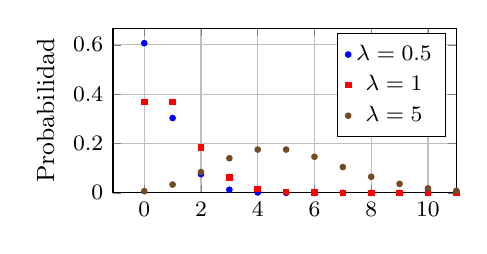
\begin{tikzpicture}
                \begin{axis}[
                    footnotesize,
                    %clip=false,
                    %domain=-2:2,
                    ymin=0,
                    %ymax=1,
                    xmax=11,
                    ylabel=Probabilidad,
                    samples at={0,...,11},
                    legend entries={$\lambda = 0.5$\\$\lambda = 1$\\$\lambda = 5$\\},
                    legend pos=north east,
                    legend style={font=\footnotesize},
                    width=0.49\textwidth,
                    height=0.49\textwidth/1.618,
                    %axis lines=middle,
                    grid=major,
                    mark size=1pt,
                    %no markers,
                    ]
                    \addplot+[only marks] {(0.5^x) * exp(-0.5) / factorial(x)};
                    \addplot+[only marks] {(1^x) * exp(-1) / factorial(x)};
                    \addplot+[only marks] {(5^x) * exp(-5) / factorial(x)};
                \end{axis}
            \end{tikzpicture}
            &
            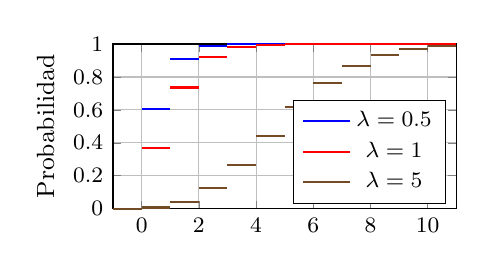
\begin{tikzpicture}
                \begin{axis}[
                    footnotesize,
                    clip=false,
                    ymin=0,
                    ymax=1,
                    xmin=-1,
                    xmax=11,
                    %samples at={0,...,11},
                    ylabel=Probabilidad,
                    legend entries={$\lambda = 0.5$\\$\lambda = 1$\\$\lambda = 5$\\},
                    legend pos=south east,
                    legend style={font=\footnotesize},
                    width=0.49\textwidth,
                    height=0.49\textwidth/1.618,
                    %axis lines=middle,
                    grid=major,
                    no markers,
                    ]
                    \addplot+[thick, jump mark left] coordinates {(-1, 0)
                        (0, {exp(-0.5)})
                        (1, {(0.5^1) * exp(-0.5) / factorial(1) + exp(-0.5)})
                        (2, {(0.5^2) * exp(-0.5) / factorial(2) + (0.5^1) * exp(-0.5) / factorial(1) + exp(-0.5)})
                        (3, {(0.5^3) * exp(-0.5) / factorial(3) + (0.5^2) * exp(-0.5) / factorial(2) + (0.5^1) * exp(-0.5) / factorial(1) + exp(-0.5)})
                        (4, {(0.5^4) * exp(-0.5) / factorial(4) + (0.5^3) * exp(-0.5) / factorial(3) + (0.5^2) * exp(-0.5) / factorial(2) + (0.5^1) * exp(-0.5) / factorial(1) + exp(-0.5)})
                        (5, {(0.5^5) * exp(-0.5) / factorial(5) + (0.5^4) * exp(-0.5) / factorial(4) + (0.5^3) * exp(-0.5) / factorial(3) + (0.5^2) * exp(-0.5) / factorial(2) + (0.5^1) * exp(-0.5) / factorial(1) + exp(-0.5)})
                        (6, {(0.5^6) * exp(-0.5) / factorial(6) + (0.5^5) * exp(-0.5) / factorial(5) + (0.5^4) * exp(-0.5) / factorial(4) + (0.5^3) * exp(-0.5) / factorial(3) + (0.5^2) * exp(-0.5) / factorial(2) + (0.5^1) * exp(-0.5) / factorial(1) + exp(-0.5)})
                        (7, {(0.5^7) * exp(-0.5) / factorial(7) + (0.5^6) * exp(-0.5) / factorial(6) + (0.5^5) * exp(-0.5) / factorial(5) + (0.5^4) * exp(-0.5) / factorial(4) + (0.5^3) * exp(-0.5) / factorial(3) + (0.5^2) * exp(-0.5) / factorial(2) + (0.5^1) * exp(-0.5) / factorial(1) + exp(-0.5)})
                        (8, {(0.5^8) * exp(-0.5) / factorial(8) + (0.5^7) * exp(-0.5) / factorial(7) + (0.5^6) * exp(-0.5) / factorial(6) + (0.5^5) * exp(-0.5) / factorial(5) + (0.5^4) * exp(-0.5) / factorial(4) + (0.5^3) * exp(-0.5) / factorial(3) + (0.5^2) * exp(-0.5) / factorial(2) + (0.5^1) * exp(-0.5) / factorial(1) + exp(-0.5)})
                        (9, {(0.5^9) * exp(-0.5) / factorial(9) + (0.5^8) * exp(-0.5) / factorial(8) + (0.5^7) * exp(-0.5) / factorial(7) + (0.5^6) * exp(-0.5) / factorial(6) + (0.5^5) * exp(-0.5) / factorial(5) + (0.5^4) * exp(-0.5) / factorial(4) + (0.5^3) * exp(-0.5) / factorial(3) + (0.5^2) * exp(-0.5) / factorial(2) + (0.5^1) * exp(-0.5) / factorial(1) + exp(-0.5)})
                        (10, {(0.5^10) * exp(-0.5) / factorial(10) + (0.5^9) * exp(-0.5) / factorial(9) + (0.5^8) * exp(-0.5) / factorial(8) + (0.5^7) * exp(-0.5) / factorial(7) + (0.5^6) * exp(-0.5) / factorial(6) + (0.5^5) * exp(-0.5) / factorial(5) + (0.5^4) * exp(-0.5) / factorial(4) + (0.5^3) * exp(-0.5) / factorial(3) + (0.5^2) * exp(-0.5) / factorial(2) + (0.5^1) * exp(-0.5) / factorial(1) + exp(-0.5)})
                        (11, {(0.5^11) * exp(-0.5) / factorial(11) + (0.5^10) * exp(-0.5) / factorial(10) + (0.5^9) * exp(-0.5) / factorial(9) + (0.5^8) * exp(-0.5) / factorial(8) + (0.5^7) * exp(-0.5) / factorial(7) + (0.5^6) * exp(-0.5) / factorial(6) + (0.5^5) * exp(-0.5) / factorial(5) + (0.5^4) * exp(-0.5) / factorial(4) + (0.5^3) * exp(-0.5) / factorial(3) + (0.5^2) * exp(-0.5) / factorial(2) + (0.5^1) * exp(-0.5) / factorial(1) + exp(-0.5)})};
                    \addplot+[thick, jump mark left] coordinates {(-1, 0)
                        (0, {exp(-1)})
                        (1, {(1^1) * exp(-1) / factorial(1) + exp(-1)})
                        (2, {(1^2) * exp(-1) / factorial(2) + (1^1) * exp(-1) / factorial(1) + exp(-1)})
                        (3, {(1^3) * exp(-1) / factorial(3) + (1^2) * exp(-1) / factorial(2) + (1^1) * exp(-1) / factorial(1) + exp(-1)})
                        (4, {(1^4) * exp(-1) / factorial(4) + (1^3) * exp(-1) / factorial(3) + (1^2) * exp(-1) / factorial(2) + (1^1) * exp(-1) / factorial(1) + exp(-1)})
                        (5, {(1^5) * exp(-1) / factorial(5) + (1^4) * exp(-1) / factorial(4) + (1^3) * exp(-1) / factorial(3) + (1^2) * exp(-1) / factorial(2) + (1^1) * exp(-1) / factorial(1) + exp(-1)})
                        (6, {(1^6) * exp(-1) / factorial(6) + (1^5) * exp(-1) / factorial(5) + (1^4) * exp(-1) / factorial(4) + (1^3) * exp(-1) / factorial(3) + (1^2) * exp(-1) / factorial(2) + (1^1) * exp(-1) / factorial(1) + exp(-1)})
                        (7, {(1^7) * exp(-1) / factorial(7) + (1^6) * exp(-1) / factorial(6) + (1^5) * exp(-1) / factorial(5) + (1^4) * exp(-1) / factorial(4) + (1^3) * exp(-1) / factorial(3) + (1^2) * exp(-1) / factorial(2) + (1^1) * exp(-1) / factorial(1) + exp(-1)})
                        (8, {(1^8) * exp(-1) / factorial(8) + (1^7) * exp(-1) / factorial(7) + (1^6) * exp(-1) / factorial(6) + (1^5) * exp(-1) / factorial(5) + (1^4) * exp(-1) / factorial(4) + (1^3) * exp(-1) / factorial(3) + (1^2) * exp(-1) / factorial(2) + (1^1) * exp(-1) / factorial(1) + exp(-1)})
                        (9, {(1^9) * exp(-1) / factorial(9) + (1^8) * exp(-1) / factorial(8) + (1^7) * exp(-1) / factorial(7) + (1^6) * exp(-1) / factorial(6) + (1^5) * exp(-1) / factorial(5) + (1^4) * exp(-1) / factorial(4) + (1^3) * exp(-1) / factorial(3) + (1^2) * exp(-1) / factorial(2) + (1^1) * exp(-1) / factorial(1) + exp(-1)})
                        (10, {(1^10) * exp(-1) / factorial(10) + (1^9) * exp(-1) / factorial(9) + (1^8) * exp(-1) / factorial(8) + (1^7) * exp(-1) / factorial(7) + (1^6) * exp(-1) / factorial(6) + (1^5) * exp(-1) / factorial(5) + (1^4) * exp(-1) / factorial(4) + (1^3) * exp(-1) / factorial(3) + (1^2) * exp(-1) / factorial(2) + (1^1) * exp(-1) / factorial(1) + exp(-1)})
                        (11, {(1^11) * exp(-1) / factorial(11) + (1^10) * exp(-1) / factorial(10) + (1^9) * exp(-1) / factorial(9) + (1^8) * exp(-1) / factorial(8) + (1^7) * exp(-1) / factorial(7) + (1^6) * exp(-1) / factorial(6) + (1^5) * exp(-1) / factorial(5) + (1^4) * exp(-1) / factorial(4) + (1^3) * exp(-1) / factorial(3) + (1^2) * exp(-1) / factorial(2) + (1^1) * exp(-1) / factorial(1) + exp(-1)})};
                    \addplot+[thick, jump mark left] coordinates {(-1, 0)
                        (0, {exp(-5)})
                        (1, {(5^1) * exp(-5) / factorial(1) + exp(-5)})
                        (2, {(5^2) * exp(-5) / factorial(2) + (5^1) * exp(-5) / factorial(1) + exp(-5)})
                        (3, {(5^3) * exp(-5) / factorial(3) + (5^2) * exp(-5) / factorial(2) + (5^1) * exp(-5) / factorial(1) + exp(-5)})
                        (4, {(5^4) * exp(-5) / factorial(4) + (5^3) * exp(-5) / factorial(3) + (5^2) * exp(-5) / factorial(2) + (5^1) * exp(-5) / factorial(1) + exp(-5)})
                        (5, {(5^5) * exp(-5) / factorial(5) + (5^4) * exp(-5) / factorial(4) + (5^3) * exp(-5) / factorial(3) + (5^2) * exp(-5) / factorial(2) + (5^1) * exp(-5) / factorial(1) + exp(-5)})
                        (6, {(5^6) * exp(-5) / factorial(6) + (5^5) * exp(-5) / factorial(5) + (5^4) * exp(-5) / factorial(4) + (5^3) * exp(-5) / factorial(3) + (5^2) * exp(-5) / factorial(2) + (5^1) * exp(-5) / factorial(1) + exp(-5)})
                        (7, {(5^7) * exp(-5) / factorial(7) + (5^6) * exp(-5) / factorial(6) + (5^5) * exp(-5) / factorial(5) + (5^4) * exp(-5) / factorial(4) + (5^3) * exp(-5) / factorial(3) + (5^2) * exp(-5) / factorial(2) + (5^1) * exp(-5) / factorial(1) + exp(-5)})
                        (8, {(5^8) * exp(-5) / factorial(8) + (5^7) * exp(-5) / factorial(7) + (5^6) * exp(-5) / factorial(6) + (5^5) * exp(-5) / factorial(5) + (5^4) * exp(-5) / factorial(4) + (5^3) * exp(-5) / factorial(3) + (5^2) * exp(-5) / factorial(2) + (5^1) * exp(-5) / factorial(1) + exp(-5)})
                        (9, {(5^9) * exp(-5) / factorial(9) + (5^8) * exp(-5) / factorial(8) + (5^7) * exp(-5) / factorial(7) + (5^6) * exp(-5) / factorial(6) + (5^5) * exp(-5) / factorial(5) + (5^4) * exp(-5) / factorial(4) + (5^3) * exp(-5) / factorial(3) + (5^2) * exp(-5) / factorial(2) + (5^1) * exp(-5) / factorial(1) + exp(-5)})
                        (10, {(5^10) * exp(-5) / factorial(10) + (5^9) * exp(-5) / factorial(9) + (5^8) * exp(-5) / factorial(8) + (5^7) * exp(-5) / factorial(7) + (5^6) * exp(-5) / factorial(6) + (5^5) * exp(-5) / factorial(5) + (5^4) * exp(-5) / factorial(4) + (5^3) * exp(-5) / factorial(3) + (5^2) * exp(-5) / factorial(2) + (5^1) * exp(-5) / factorial(1) + exp(-5)})
                        (11, {(5^11) * exp(-5) / factorial(11) + (5^10) * exp(-5) / factorial(10) + (5^9) * exp(-5) / factorial(9) + (5^8) * exp(-5) / factorial(8) + (5^7) * exp(-5) / factorial(7) + (5^6) * exp(-5) / factorial(6) + (5^5) * exp(-5) / factorial(5) + (5^4) * exp(-5) / factorial(4) + (5^3) * exp(-5) / factorial(3) + (5^2) * exp(-5) / factorial(2) + (5^1) * exp(-5) / factorial(1) + exp(-5)})};
                \end{axis}
            \end{tikzpicture}
        \end{tabular}
    \end{center}
    \begin{block}{Propiedades}
        \begin{itemize}
            \item $\expecteddist{X \sim \poisson{\lambda}}{X} = \mu_{X} = \lambda$.
            \item $\variancedist{X \sim \poisson{\lambda}}{X} = \sigma^{2}_{X} = \lambda$.
        \end{itemize}
    \end{block}
\end{frame}

%%%%%%%


\begin{frame}
    \frametitle{Distribución $X \sim \text{Poisson} \parens{\lambda} = \poisson{\lambda}$}
    \begin{center}
        \begin{tabular}{cc}
            \emph{pmf} ($\ff{x}$) & \emph{cdf} ($\FF{x}$) \\
            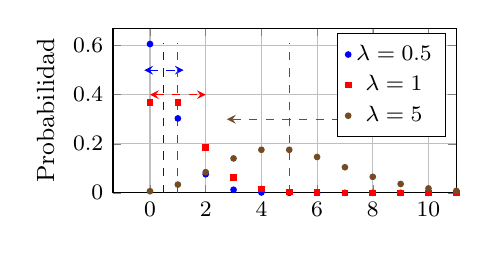
\begin{tikzpicture}
                \begin{axis}[
                    footnotesize,
                    %clip=false,
                    %domain=-2:2,
                    ymin=0,
                    %ymax=1,
                    xmax=11,
                    ylabel=Probabilidad,
                    samples at={0,...,11},
                    legend entries={$\lambda = 0.5$\\$\lambda = 1$\\$\lambda = 5$\\},
                    legend pos=north east,
                    legend style={font=\footnotesize},
                    width=0.49\textwidth,
                    height=0.49\textwidth/1.618,
                    %axis lines=middle,
                    grid=major,
                    mark size=1pt,
                    %no markers,
                    ]
                    \addplot+[forget plot, dashed, no markers] coordinates {(0.5, 0) (0.5, 0.61)};
                    \addplot+[forget plot, dashed, no markers, stealth-stealth] coordinates {(0.5 - sqrt(0.5), 0.5) (0.5 + sqrt(0.5), 0.5)};
                    \addplot+[only marks] {(0.5^x) * exp(-0.5) / factorial(x)};
                    \addplot+[forget plot, dashed, no markers] coordinates {(1, 0) (1, 0.61)};
                    \addplot+[forget plot, dashed, no markers, stealth-stealth] coordinates {(1 - 1, 0.4) (1 + 1, 0.4)};
                    \addplot+[only marks] {(1^x) * exp(-1) / factorial(x)};
                    \addplot+[forget plot, dashed, no markers] coordinates {(5, 0) (5, 0.61)};
                    \addplot+[forget plot, dashed, no markers, stealth-stealth] coordinates {(5 - sqrt(5), 0.3) (5 + sqrt(5), 0.3)};
                    \addplot+[only marks] {(5^x) * exp(-5) / factorial(x)};
                \end{axis}
            \end{tikzpicture}
            &
            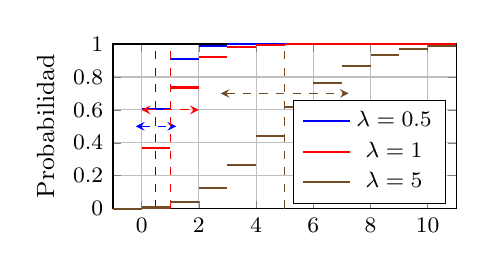
\begin{tikzpicture}
                \begin{axis}[
                    footnotesize,
                    clip=false,
                    ymin=0,
                    ymax=1,
                    xmin=-1,
                    xmax=11,
                    %samples at={0,...,11},
                    ylabel=Probabilidad,
                    legend entries={$\lambda = 0.5$\\$\lambda = 1$\\$\lambda = 5$\\},
                    legend pos=south east,
                    legend style={font=\footnotesize},
                    width=0.49\textwidth,
                    height=0.49\textwidth/1.618,
                    %axis lines=middle,
                    grid=major,
                    no markers,
                    ]
                    \addplot+[forget plot, dashed] coordinates {(0.5, 0) (0.5, 1)};
                    \addplot+[forget plot, dashed, stealth-stealth] coordinates {(0.5 - sqrt(0.5), 0.5) (0.5 + sqrt(0.5), 0.5)};
                    \addplot+[thick, jump mark left] coordinates {(-1, 0)
                        (0, {exp(-0.5)})
                        (1, {(0.5^1) * exp(-0.5) / factorial(1) + exp(-0.5)})
                        (2, {(0.5^2) * exp(-0.5) / factorial(2) + (0.5^1) * exp(-0.5) / factorial(1) + exp(-0.5)})
                        (3, {(0.5^3) * exp(-0.5) / factorial(3) + (0.5^2) * exp(-0.5) / factorial(2) + (0.5^1) * exp(-0.5) / factorial(1) + exp(-0.5)})
                        (4, {(0.5^4) * exp(-0.5) / factorial(4) + (0.5^3) * exp(-0.5) / factorial(3) + (0.5^2) * exp(-0.5) / factorial(2) + (0.5^1) * exp(-0.5) / factorial(1) + exp(-0.5)})
                        (5, {(0.5^5) * exp(-0.5) / factorial(5) + (0.5^4) * exp(-0.5) / factorial(4) + (0.5^3) * exp(-0.5) / factorial(3) + (0.5^2) * exp(-0.5) / factorial(2) + (0.5^1) * exp(-0.5) / factorial(1) + exp(-0.5)})
                        (6, {(0.5^6) * exp(-0.5) / factorial(6) + (0.5^5) * exp(-0.5) / factorial(5) + (0.5^4) * exp(-0.5) / factorial(4) + (0.5^3) * exp(-0.5) / factorial(3) + (0.5^2) * exp(-0.5) / factorial(2) + (0.5^1) * exp(-0.5) / factorial(1) + exp(-0.5)})
                        (7, {(0.5^7) * exp(-0.5) / factorial(7) + (0.5^6) * exp(-0.5) / factorial(6) + (0.5^5) * exp(-0.5) / factorial(5) + (0.5^4) * exp(-0.5) / factorial(4) + (0.5^3) * exp(-0.5) / factorial(3) + (0.5^2) * exp(-0.5) / factorial(2) + (0.5^1) * exp(-0.5) / factorial(1) + exp(-0.5)})
                        (8, {(0.5^8) * exp(-0.5) / factorial(8) + (0.5^7) * exp(-0.5) / factorial(7) + (0.5^6) * exp(-0.5) / factorial(6) + (0.5^5) * exp(-0.5) / factorial(5) + (0.5^4) * exp(-0.5) / factorial(4) + (0.5^3) * exp(-0.5) / factorial(3) + (0.5^2) * exp(-0.5) / factorial(2) + (0.5^1) * exp(-0.5) / factorial(1) + exp(-0.5)})
                        (9, {(0.5^9) * exp(-0.5) / factorial(9) + (0.5^8) * exp(-0.5) / factorial(8) + (0.5^7) * exp(-0.5) / factorial(7) + (0.5^6) * exp(-0.5) / factorial(6) + (0.5^5) * exp(-0.5) / factorial(5) + (0.5^4) * exp(-0.5) / factorial(4) + (0.5^3) * exp(-0.5) / factorial(3) + (0.5^2) * exp(-0.5) / factorial(2) + (0.5^1) * exp(-0.5) / factorial(1) + exp(-0.5)})
                        (10, {(0.5^10) * exp(-0.5) / factorial(10) + (0.5^9) * exp(-0.5) / factorial(9) + (0.5^8) * exp(-0.5) / factorial(8) + (0.5^7) * exp(-0.5) / factorial(7) + (0.5^6) * exp(-0.5) / factorial(6) + (0.5^5) * exp(-0.5) / factorial(5) + (0.5^4) * exp(-0.5) / factorial(4) + (0.5^3) * exp(-0.5) / factorial(3) + (0.5^2) * exp(-0.5) / factorial(2) + (0.5^1) * exp(-0.5) / factorial(1) + exp(-0.5)})
                        (11, {(0.5^11) * exp(-0.5) / factorial(11) + (0.5^10) * exp(-0.5) / factorial(10) + (0.5^9) * exp(-0.5) / factorial(9) + (0.5^8) * exp(-0.5) / factorial(8) + (0.5^7) * exp(-0.5) / factorial(7) + (0.5^6) * exp(-0.5) / factorial(6) + (0.5^5) * exp(-0.5) / factorial(5) + (0.5^4) * exp(-0.5) / factorial(4) + (0.5^3) * exp(-0.5) / factorial(3) + (0.5^2) * exp(-0.5) / factorial(2) + (0.5^1) * exp(-0.5) / factorial(1) + exp(-0.5)})};
                    \addplot+[forget plot, dashed] coordinates {(1, 0) (1, 1)};
                    \addplot+[forget plot, dashed, stealth-stealth] coordinates {(1 - 1, 0.6) (1 + 1, 0.6)};
                    \addplot+[thick, jump mark left] coordinates {(-1, 0)
                        (0, {exp(-1)})
                        (1, {(1^1) * exp(-1) / factorial(1) + exp(-1)})
                        (2, {(1^2) * exp(-1) / factorial(2) + (1^1) * exp(-1) / factorial(1) + exp(-1)})
                        (3, {(1^3) * exp(-1) / factorial(3) + (1^2) * exp(-1) / factorial(2) + (1^1) * exp(-1) / factorial(1) + exp(-1)})
                        (4, {(1^4) * exp(-1) / factorial(4) + (1^3) * exp(-1) / factorial(3) + (1^2) * exp(-1) / factorial(2) + (1^1) * exp(-1) / factorial(1) + exp(-1)})
                        (5, {(1^5) * exp(-1) / factorial(5) + (1^4) * exp(-1) / factorial(4) + (1^3) * exp(-1) / factorial(3) + (1^2) * exp(-1) / factorial(2) + (1^1) * exp(-1) / factorial(1) + exp(-1)})
                        (6, {(1^6) * exp(-1) / factorial(6) + (1^5) * exp(-1) / factorial(5) + (1^4) * exp(-1) / factorial(4) + (1^3) * exp(-1) / factorial(3) + (1^2) * exp(-1) / factorial(2) + (1^1) * exp(-1) / factorial(1) + exp(-1)})
                        (7, {(1^7) * exp(-1) / factorial(7) + (1^6) * exp(-1) / factorial(6) + (1^5) * exp(-1) / factorial(5) + (1^4) * exp(-1) / factorial(4) + (1^3) * exp(-1) / factorial(3) + (1^2) * exp(-1) / factorial(2) + (1^1) * exp(-1) / factorial(1) + exp(-1)})
                        (8, {(1^8) * exp(-1) / factorial(8) + (1^7) * exp(-1) / factorial(7) + (1^6) * exp(-1) / factorial(6) + (1^5) * exp(-1) / factorial(5) + (1^4) * exp(-1) / factorial(4) + (1^3) * exp(-1) / factorial(3) + (1^2) * exp(-1) / factorial(2) + (1^1) * exp(-1) / factorial(1) + exp(-1)})
                        (9, {(1^9) * exp(-1) / factorial(9) + (1^8) * exp(-1) / factorial(8) + (1^7) * exp(-1) / factorial(7) + (1^6) * exp(-1) / factorial(6) + (1^5) * exp(-1) / factorial(5) + (1^4) * exp(-1) / factorial(4) + (1^3) * exp(-1) / factorial(3) + (1^2) * exp(-1) / factorial(2) + (1^1) * exp(-1) / factorial(1) + exp(-1)})
                        (10, {(1^10) * exp(-1) / factorial(10) + (1^9) * exp(-1) / factorial(9) + (1^8) * exp(-1) / factorial(8) + (1^7) * exp(-1) / factorial(7) + (1^6) * exp(-1) / factorial(6) + (1^5) * exp(-1) / factorial(5) + (1^4) * exp(-1) / factorial(4) + (1^3) * exp(-1) / factorial(3) + (1^2) * exp(-1) / factorial(2) + (1^1) * exp(-1) / factorial(1) + exp(-1)})
                        (11, {(1^11) * exp(-1) / factorial(11) + (1^10) * exp(-1) / factorial(10) + (1^9) * exp(-1) / factorial(9) + (1^8) * exp(-1) / factorial(8) + (1^7) * exp(-1) / factorial(7) + (1^6) * exp(-1) / factorial(6) + (1^5) * exp(-1) / factorial(5) + (1^4) * exp(-1) / factorial(4) + (1^3) * exp(-1) / factorial(3) + (1^2) * exp(-1) / factorial(2) + (1^1) * exp(-1) / factorial(1) + exp(-1)})};
                    \addplot+[forget plot, dashed] coordinates {(5, 0) (5, 1)};
                    \addplot+[forget plot, dashed, stealth-stealth] coordinates {(5 - sqrt(5), 0.7) (5 + sqrt(5), 0.7)};
                    \addplot+[thick, jump mark left] coordinates {(-1, 0)
                        (0, {exp(-5)})
                        (1, {(5^1) * exp(-5) / factorial(1) + exp(-5)})
                        (2, {(5^2) * exp(-5) / factorial(2) + (5^1) * exp(-5) / factorial(1) + exp(-5)})
                        (3, {(5^3) * exp(-5) / factorial(3) + (5^2) * exp(-5) / factorial(2) + (5^1) * exp(-5) / factorial(1) + exp(-5)})
                        (4, {(5^4) * exp(-5) / factorial(4) + (5^3) * exp(-5) / factorial(3) + (5^2) * exp(-5) / factorial(2) + (5^1) * exp(-5) / factorial(1) + exp(-5)})
                        (5, {(5^5) * exp(-5) / factorial(5) + (5^4) * exp(-5) / factorial(4) + (5^3) * exp(-5) / factorial(3) + (5^2) * exp(-5) / factorial(2) + (5^1) * exp(-5) / factorial(1) + exp(-5)})
                        (6, {(5^6) * exp(-5) / factorial(6) + (5^5) * exp(-5) / factorial(5) + (5^4) * exp(-5) / factorial(4) + (5^3) * exp(-5) / factorial(3) + (5^2) * exp(-5) / factorial(2) + (5^1) * exp(-5) / factorial(1) + exp(-5)})
                        (7, {(5^7) * exp(-5) / factorial(7) + (5^6) * exp(-5) / factorial(6) + (5^5) * exp(-5) / factorial(5) + (5^4) * exp(-5) / factorial(4) + (5^3) * exp(-5) / factorial(3) + (5^2) * exp(-5) / factorial(2) + (5^1) * exp(-5) / factorial(1) + exp(-5)})
                        (8, {(5^8) * exp(-5) / factorial(8) + (5^7) * exp(-5) / factorial(7) + (5^6) * exp(-5) / factorial(6) + (5^5) * exp(-5) / factorial(5) + (5^4) * exp(-5) / factorial(4) + (5^3) * exp(-5) / factorial(3) + (5^2) * exp(-5) / factorial(2) + (5^1) * exp(-5) / factorial(1) + exp(-5)})
                        (9, {(5^9) * exp(-5) / factorial(9) + (5^8) * exp(-5) / factorial(8) + (5^7) * exp(-5) / factorial(7) + (5^6) * exp(-5) / factorial(6) + (5^5) * exp(-5) / factorial(5) + (5^4) * exp(-5) / factorial(4) + (5^3) * exp(-5) / factorial(3) + (5^2) * exp(-5) / factorial(2) + (5^1) * exp(-5) / factorial(1) + exp(-5)})
                        (10, {(5^10) * exp(-5) / factorial(10) + (5^9) * exp(-5) / factorial(9) + (5^8) * exp(-5) / factorial(8) + (5^7) * exp(-5) / factorial(7) + (5^6) * exp(-5) / factorial(6) + (5^5) * exp(-5) / factorial(5) + (5^4) * exp(-5) / factorial(4) + (5^3) * exp(-5) / factorial(3) + (5^2) * exp(-5) / factorial(2) + (5^1) * exp(-5) / factorial(1) + exp(-5)})
                        (11, {(5^11) * exp(-5) / factorial(11) + (5^10) * exp(-5) / factorial(10) + (5^9) * exp(-5) / factorial(9) + (5^8) * exp(-5) / factorial(8) + (5^7) * exp(-5) / factorial(7) + (5^6) * exp(-5) / factorial(6) + (5^5) * exp(-5) / factorial(5) + (5^4) * exp(-5) / factorial(4) + (5^3) * exp(-5) / factorial(3) + (5^2) * exp(-5) / factorial(2) + (5^1) * exp(-5) / factorial(1) + exp(-5)})};
                \end{axis}
            \end{tikzpicture}
        \end{tabular}
    \end{center}
    \begin{block}{Propiedades}
        \begin{itemize}
            \item $\expecteddist{X \sim \poisson{\lambda}}{X} = \mu_{X} = \lambda$.
            \item $\variancedist{X \sim \poisson{\lambda}}{X} = \sigma^{2}_{X} = \lambda$.
        \end{itemize}
    \end{block}
\end{frame}


%%%%%%%%%



\begin{frame}
    \begin{center}
        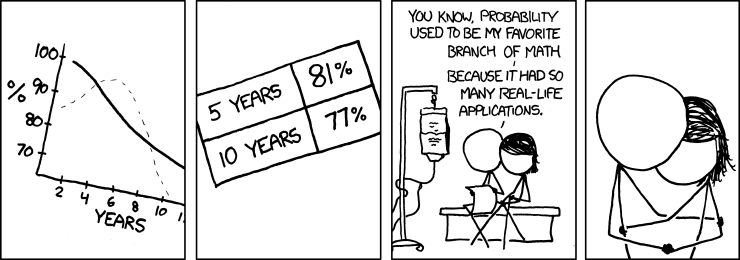
\includegraphics[width=0.95\textwidth]{xkcd_probability}
    \end{center}
\end{frame}

\begin{frame}
    \frametitle{Variables aleatorias continuas}
    \begin{exampleblock}{Ejemplo}
        \begin{itemize}
            \item ¿Cómo se distribuyen los tiempos de espera en la fila para almorzar?
        \end{itemize}
    \end{exampleblock}
    \begin{block}{Solución 1: discretizar en clases intervalos de ancho $a = 1$}
        \begin{itemize}
            \item $\text{Clases}_{a = 1} = \bparens{\sparens{0 , 1}, \left ( 1, 2 \right ] , \left ( 2, 3 \right ] , \ldots}$.
            \item Se cumple que:
            \begin{equation*}
                \prob{X \in \sparens{0, 1}} + \sum_{i = 1}^{+ \infty} \prob{X \in \left ( i, i + 1 \right ]} = 1 .
            \end{equation*}
        \end{itemize}
    \end{block}
    \begin{center}
        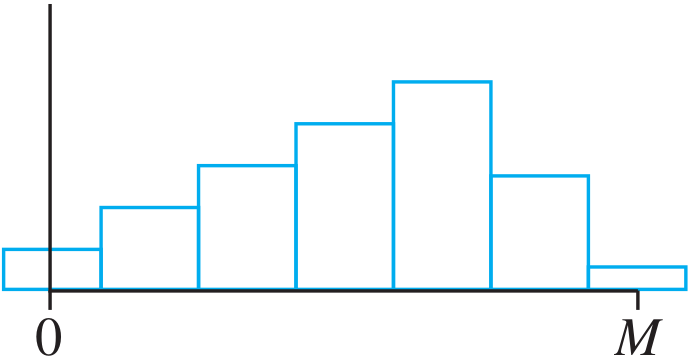
\includegraphics[width=0.45\textwidth]{continua_1}
    \end{center}
\end{frame}

\begin{frame}
    \frametitle{Variables aleatorias continuas}
    \begin{block}{Solución $\frac{1}{2}$: discretizar en clases intervalos de ancho $a = \frac{1}{2}$}
        \begin{itemize}
            \item $\text{Clases}_{a = \frac{1}{2}} = \bparens{\sparens{0 , \frac{1}{2}}, \left ( \frac{1}{2} , 1 \right ] , \left ( 1 , \frac{3}{2} \right ] , \ldots}$.
            \item Se cumple que:
                \begin{equation*}
                    \prob{X \in \sparens{0, \frac{1}{2}}} + \sum_{i = 1}^{+ \infty} \prob{X \in \left ( \frac{i}{2}, \frac{i + 1}{2} \right ]} = 1 .
                \end{equation*}
        \end{itemize}
    \end{block}
    \begin{center}
        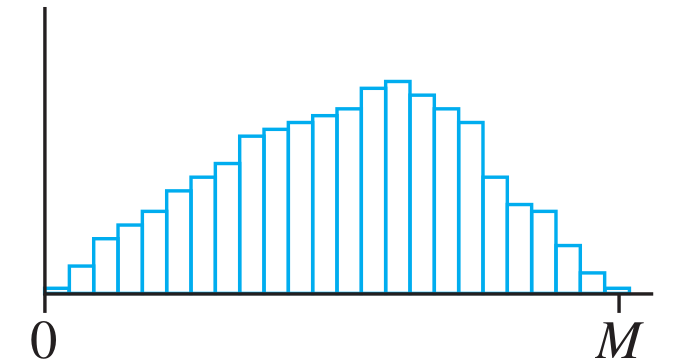
\includegraphics[width=0.45\textwidth]{continua_2}
    \end{center}
\end{frame}

\begin{frame}
    \frametitle{Variables aleatorias continuas}
    \begin{block}{Solución $a$}
        \begin{itemize}
            \item $\text{Clases}_{a} = \bparens{\sparens{0 , a}, \left ( a , 2 a \right ] , \left ( 2 a , 3 a \right ] , \ldots}$.
            \item Se cumple que:
                \begin{equation*}
                    \prob{X \in \sparens{0, a}} + \sum_{i = 1}^{+ \infty} \prob{X \in \left ( i a, \parens{i + 1} a \right ]} = 1 .
                \end{equation*}
            \item Recordando que $\prob{X \leq x} = \FF{x}$, se puede reescribir como:
                \begin{equation*}
                    \FF{a} + \sum_{i = 1}^{+ \infty} \FF{\parens{i + 1} a} - \FF{i a} = 1 .
                \end{equation*}
        \end{itemize}
    \end{block}
    \begin{center}
        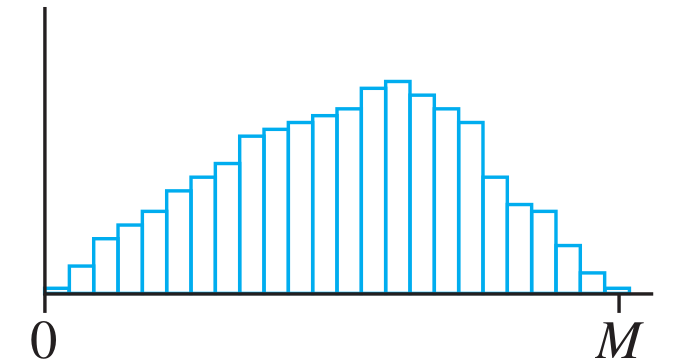
\includegraphics[width=0.45\textwidth]{continua_2}
    \end{center}
\end{frame}



\begin{frame}
    \frametitle{Variables aleatorias continuas}
    \begin{block}{Solución $a$}
        \begin{itemize}
            \item Se tiene que:
                \begin{equation*}
                    \FF{a} + \sum_{i = 1}^{+ \infty} \FF{\parens{i + 1} a} - \FF{i a} =
                    \FF{a} + \sum_{i = 1}^{+ \infty} \text{Área} \parens{i} = 1 ,
                \end{equation*}
                \begin{equation*}
                    \text{con } \text{Área} \parens{i} = h_{i} a = \prob{X \in \left ( i a, \parens{i + 1} a \right ]} = \FF{\parens{i + 1} a} - \FF{i a} .
                \end{equation*}
            \item Notar que la altura cumple:
                \begin{equation*}
                    h_{i} = \frac{\FF{i a + a} - \FF{i a}}{a} .
                \end{equation*}
        \end{itemize}
    \end{block}
    \begin{center}
        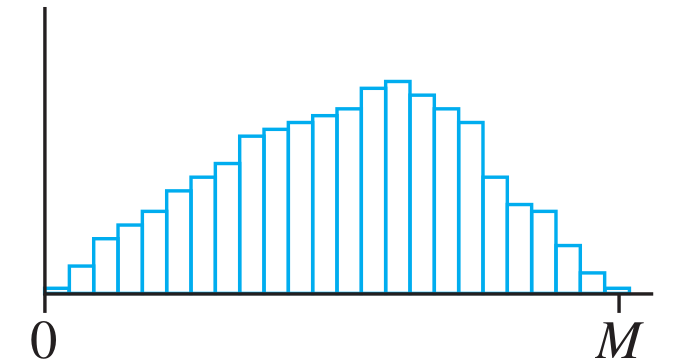
\includegraphics[width=0.45\textwidth]{continua_2}
    \end{center}
\end{frame}

\begin{frame}
    \frametitle{Variables aleatorias continuas}
    \begin{block}{Solución $a \rightarrow 0$}
        \begin{equation*}
            h_{x} = \lim_{a \rightarrow 0} \frac{\FF{x + a} - \FF{x}}{a} , \text{ y }
            \int_{x \in E} h_{x} d x = 1 .
        \end{equation*}
    \end{block}
    \begin{center}
        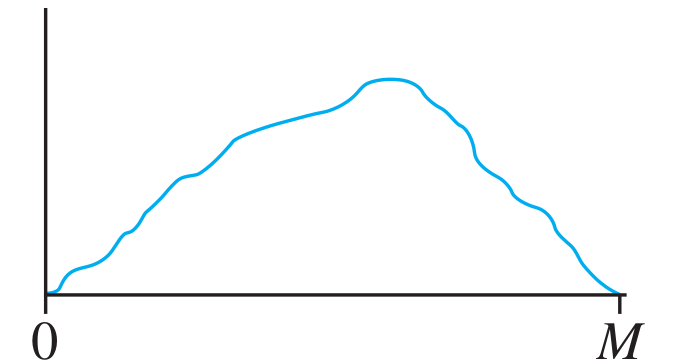
\includegraphics[width=0.45\textwidth]{continua_3}
    \end{center}
    \begin{block}{Función de densidad de probabilidad (\emph{pdf})}
        \begin{itemize}
            \item $\pdf{x} \equiv h_{x}$.
            \item Debe cumplir:
                \begin{itemize}
                    \item $\forall x \in E , \pdf{x} \geq 0$. $\int_{x \in E} \pdf{x} d x = 1$.
                    
                \end{itemize}
        \end{itemize}
    \end{block}
\end{frame}



%%%%%%%)==)=)=)


\begin{frame}
    \frametitle{Variables aleatorias continuas -- definiciones}
    \begin{block}{Función de densidad de probabilidad (\emph{pdf})}
        \begin{equation*}
            \prob{a \leq X \leq b} = \int_{a}^{b} \pdf{x} d x .
        \end{equation*}
    \end{block}
    \begin{block}{Función de distribución acumulada (\emph{cdf})}
        \begin{equation*}
            \FF{x} = \prob{X \leq x} = \int_{- \infty}^{x} \pdf{t} d t .
        \end{equation*}
    \end{block}
    \begin{center}
        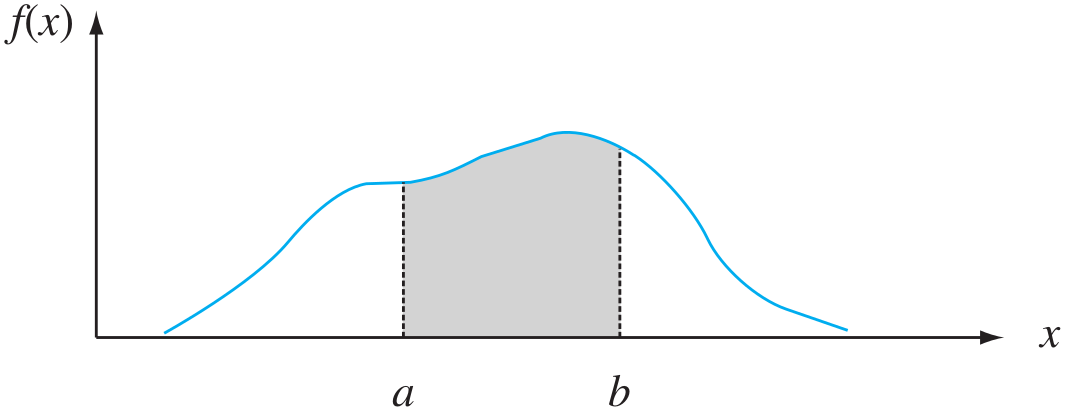
\includegraphics[width=0.6\textwidth]{pdf_interval}
    \end{center}
\end{frame}

\begin{frame}
    \frametitle{Variables aleatorias continuas -- definiciones}
    \begin{block}{Valor esperado / esperanza}
        \begin{equation*}
            \expecteddist{X \sim p}{X} = \mu_{X} = \int_{x \in E} x \pdf{x} d x .
        \end{equation*}
    \end{block}
    \begin{block}{Varianza}
        \begin{equation*}
            \variancedist{X \sim p}{X} = \sigma^{2}_{X} = \int_{x \in E} \parens{x - \expected{X}}^{2} \pdf{x} d x .
        \end{equation*}
    \end{block}
    \begin{center}
        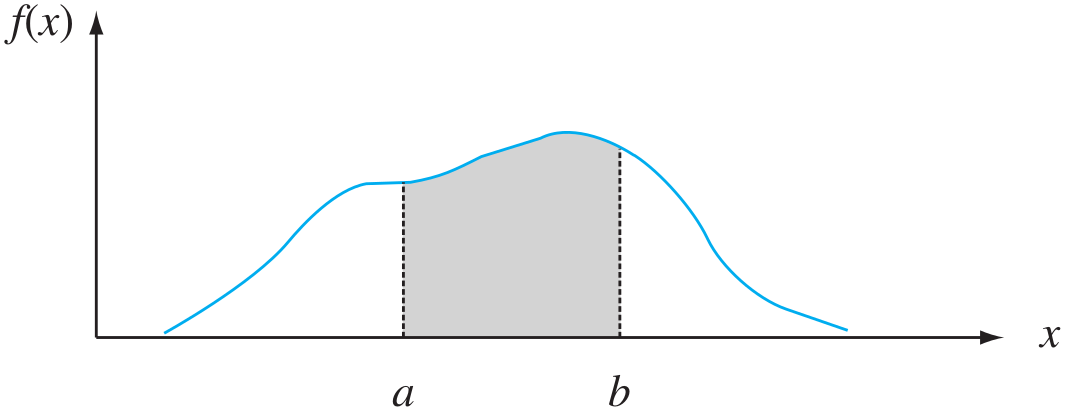
\includegraphics[width=0.6\textwidth]{pdf_interval}
    \end{center}
\end{frame}

\begin{frame}
    \frametitle{Variables aleatorias continuas -- definiciones}
    \begin{block}{Cuantil / percentil}
        \begin{itemize}
            \item $q_{u}$ tal que
                \begin{equation*}
                    \prob{X \leq q_{u}} = \FF{q_{u}} = \int_{- \infty}^{q_{u}} \pdf{x} d x = u .
                \end{equation*}
        \end{itemize}
    \end{block}
    \begin{center}
        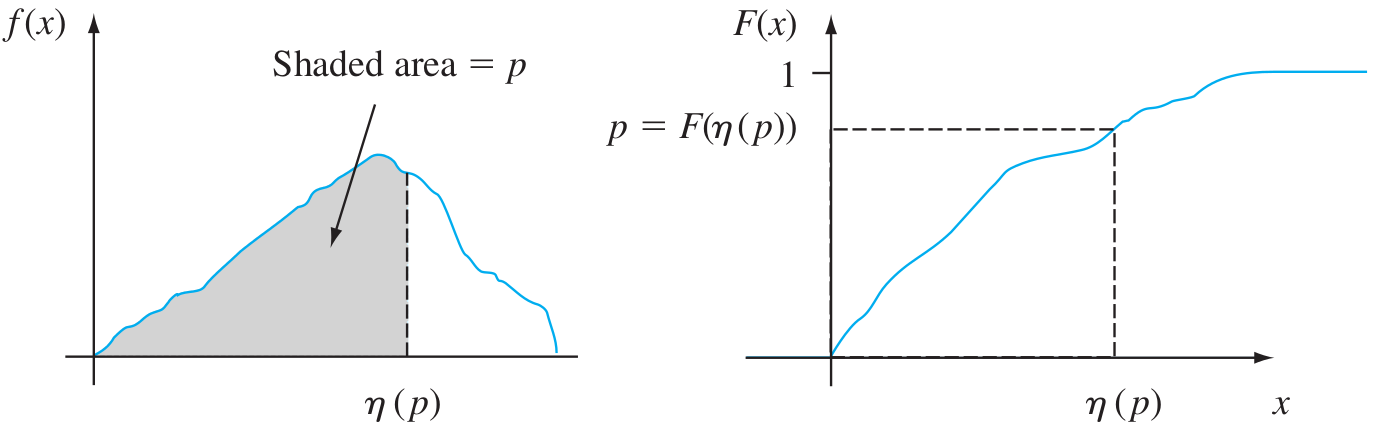
\includegraphics[width=\textwidth]{percentile}
    \end{center}
    \begin{alertblock}{}
        \begin{itemize}
            \item En esta figura, $\ff{x} = \pdf{x}$, $p = u$, $\eta \parens{p} = q_{u}$.
        \end{itemize}
    \end{alertblock}
\end{frame}

\begin{frame}
    \frametitle{Distribución $X \sim \text{Uniforme} \parens{a, b} = \uniform{a}{b}$}
    \begin{block}{Ángulos}
        \begin{itemize}
            \item Ángulo luego de girar ruleta.
            \item Ángulo desde el centro al lanzar un dardo.
        \end{itemize}
    \end{block}
    \begin{block}{Otros}
        \begin{itemize}
            \item Valor del parámetro $p$ en una distribución $\bernoulli{p}$.
        \end{itemize}
    \end{block}
\end{frame}

\begin{frame}
    \frametitle{Distribución $X \sim \text{Uniforme} \parens{a, b} = \uniform{a}{b}$}
    \begin{block}{Definición}
        \begin{equation*}
            \pdf{x} = \frac{1}{b - a} , \text{ con } x \in \sparens{a, b} .
        \end{equation*}
    \end{block}
    \begin{center}
        \begin{tabular}{cc}
            \emph{pdf} ($\pdf{x}$) & \emph{cdf} ($\FF{x}$) \\
            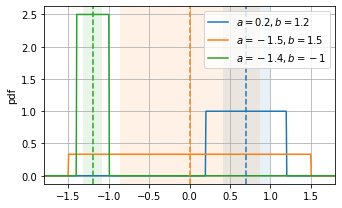
\includegraphics[width=0.42\textwidth]{pdf_uniform} &
            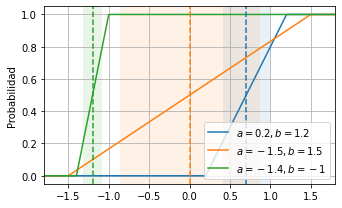
\includegraphics[width=0.42\textwidth]{cdf_uniform}
        \end{tabular}
    \end{center}
 \end{frame}


%%%%%%%%%%


\begin{frame}
    \frametitle{Distribución $X \sim \text{Uniforme} \parens{a, b} = \uniform{a}{b}$}
    \begin{block}{Propiedades}
        \begin{itemize}
            \item $\expecteddist{X \sim \uniform{a}{b}}{X} = \mu_{X} = \frac{a + b}{2}$.
            \item $\variancedist{X \sim \uniform{a}{b}}{X} = \sigma^{2}_{X} = \frac{\parens{b - a}^{2}}{12}$.
        \end{itemize}
    \end{block}
\end{frame}

\begin{frame}
    \frametitle{Ejemplo -- tiempo entre vacunados}
    \begin{block}{Supuesto}
        \begin{itemize}
            \item Número de personas que llegan a vacunatorio sigue distribución Poisson con media 12 personas por hora.
            \item Luego de llegar al vacunatorio, ¿cuál es la probabilidad de que la próxima persona llegue
                \begin{itemize}
                    \item en más de 1 hora?
                    \item en más de 15 minutos?
                    \item en más de 5 minutos?
                    \item en menos de 5 minutos?
                \end{itemize}
        \end{itemize}
    \end{block}
    \begin{block}{Recordar}
        \begin{equation*}
            X \sim \poisson{\lambda} \Rightarrow \prob{X = x} = e^{- \lambda} \frac{\lambda^{x}}{x!} .
        \end{equation*}
    \end{block}
\end{frame}


%%%%$$$


\begin{frame}
    \frametitle{Ejemplo -- tiempo entre vacunados}
    \begin{block}{Supuesto}
        \begin{itemize}
            \item Número de personas que llegan a vacunatorio sigue distribución Poisson con media 12 personas por hora.
            \item Luego de llegar al vacunatorio, ¿cuál es la probabilidad de que la próxima persona llegue...
        \end{itemize}
    \end{block}
    \begin{block}{en más de 1 hora?}
        \begin{equation*}
            X \sim \poisson{12} \Rightarrow \prob{X = x} = e^{- 12} \frac{12^{x}}{x!}
            \Rightarrow \prob{X = 0} = e^{- 12} .
        \end{equation*}
    \end{block}
    \begin{block}{en más de 15 minutos?}
        \begin{itemize}
            \item 12 personas por hora es equivalente a 3 persona cada 15 minutos.
        \end{itemize}
        \begin{equation*}
            X \sim \poisson{3} \Rightarrow \prob{X = x} = e^{- 3} \frac{3^{x}}{x!}
            \Rightarrow \prob{X = 0} = e^{- 3} .
        \end{equation*}
    \end{block}
\end{frame}

\begin{frame}
    \frametitle{Ejemplo -- tiempo entre vacunados}
    \begin{block}{Supuesto}
        \begin{itemize}
            \item Número de personas que llegan a vacunatorio sigue distribución Poisson con media 12 personas por hora.
            \item Luego de llegar al vacunatorio, ¿cuál es la probabilidad de que la próxima persona llegue...
        \end{itemize}
    \end{block}
    \begin{block}{en más de 5 minutos?}
        \begin{itemize}
            \item 12 personas por hora es equivalente a 1 persona cada 5 minutos.
        \end{itemize}
        \begin{equation*}
            X \sim \poisson{1} \Rightarrow \prob{X = x} = e^{- 1} \frac{1}{x!}
            \Rightarrow \prob{X = 0} = e^{- 1} .
        \end{equation*}
    \end{block}
    \begin{block}{en menos de 5 minutos?}
        \begin{itemize}
            \item 12 personas por hora es equivalente a 1 persona cada 5 minutos.
        \end{itemize}
        \begin{equation*}
            \prob{X = x} = e^{- 1} \frac{1}{x!}
            \Rightarrow \prob{X > 0} = 1 - \prob{X = 0} = 1 - e^{- 1} .
        \end{equation*}
    \end{block}
\end{frame}

\begin{frame}
    \frametitle{Ejemplo -- tiempo entre vacunados}
    \begin{block}{En general}
        \begin{itemize}
            \item Probabilidad de que la próxima persona llegue en más de $t$ horas.
                \begin{equation*}
                    X \sim \poisson{\lambda t} \Rightarrow \prob{X = x} = e^{- \lambda t} \frac{\parens{\lambda t}^{x}}{x!}
                    \Rightarrow \prob{X = 0} = e^{- \lambda t} .
                \end{equation*}
            \item Probabilidad de que la próxima persona llegue en menos de $t$ horas.
                \begin{equation*}
                    X \sim \poisson{\lambda t} \Rightarrow \prob{X = x} = e^{- \lambda t} \frac{\parens{\lambda t}^{x}}{x!}
                    \Rightarrow \prob{X > 0} = 1 - e^{- \lambda t} .
                \end{equation*}
        \end{itemize}
    \end{block}
\end{frame}

\begin{frame}

    \begin{block}{¿Qué pasó?}
        \begin{itemize}
            \item Estas probabilidades son funciones continuas de $t$.
            \item $e^{- \lambda 0} = 1$ y $\lim_{t \rightarrow + \infty} e^{- \lambda t} = 0$.
            \item Supongamos que existe una distribución continua de probabilidad del tiempo $T$ de llegada de siguiente persona:
                \begin{equation*}
                    \prob{T \leq t} = \FF{t} = \int_{u = 0}^{t} \pdf{u} d u = 1 - e^{- \lambda t} .
                \end{equation*}
        \end{itemize}
    \end{block}
\end{frame}


\begin{frame}
    \frametitle{Distribución $\exponential{\lambda}$}
    \begin{block}{Solución}
        \begin{equation*}
            \pdf{x} = \lambda e^{- \lambda x} .
        \end{equation*}
    \end{block}
    \begin{center}
        \begin{tabular}{cc}
            \emph{pdf} ($\pdf{x}$) & \emph{cdf} ($\FF{x}$) \\
            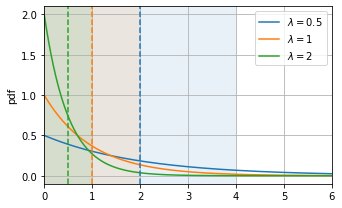
\includegraphics[width=0.42\textwidth]{pdf_exponencial} &
            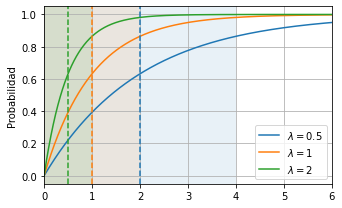
\includegraphics[width=0.42\textwidth]{cdf_exponencial}
        \end{tabular}
    \end{center}
    \begin{block}{Propiedades}
        \begin{itemize}
            \item $\expecteddist{X \sim \exponential{\lambda}}{X} = \mu_{X} = \frac{1}{\lambda}$.
            \item $\variancedist{X \sim \exponential{\lambda}}{X} = \sigma^{2}_{X} = \frac{1}{\lambda^{2}}$.
        \end{itemize}
    \end{block}
\end{frame}

\iffalse
\begin{frame}
    \frametitle{Movimientos en cancha de fútbol}
    \begin{center}
        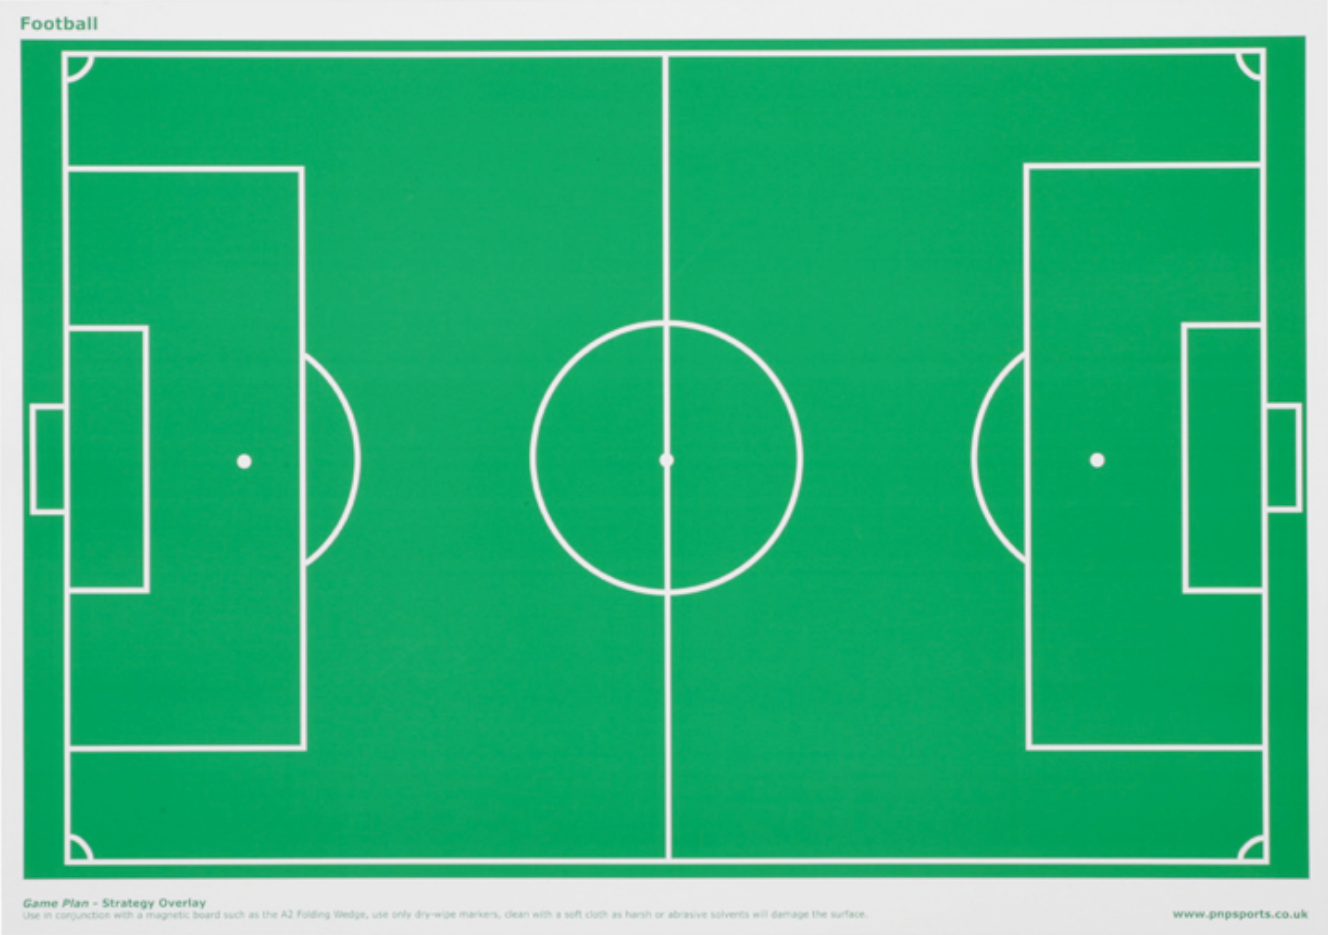
\includegraphics[width=0.9\textwidth]{futbol0}
    \end{center}
\end{frame}

\begin{frame}
    \frametitle{Movimientos en cancha de fútbol}
    \begin{center}
        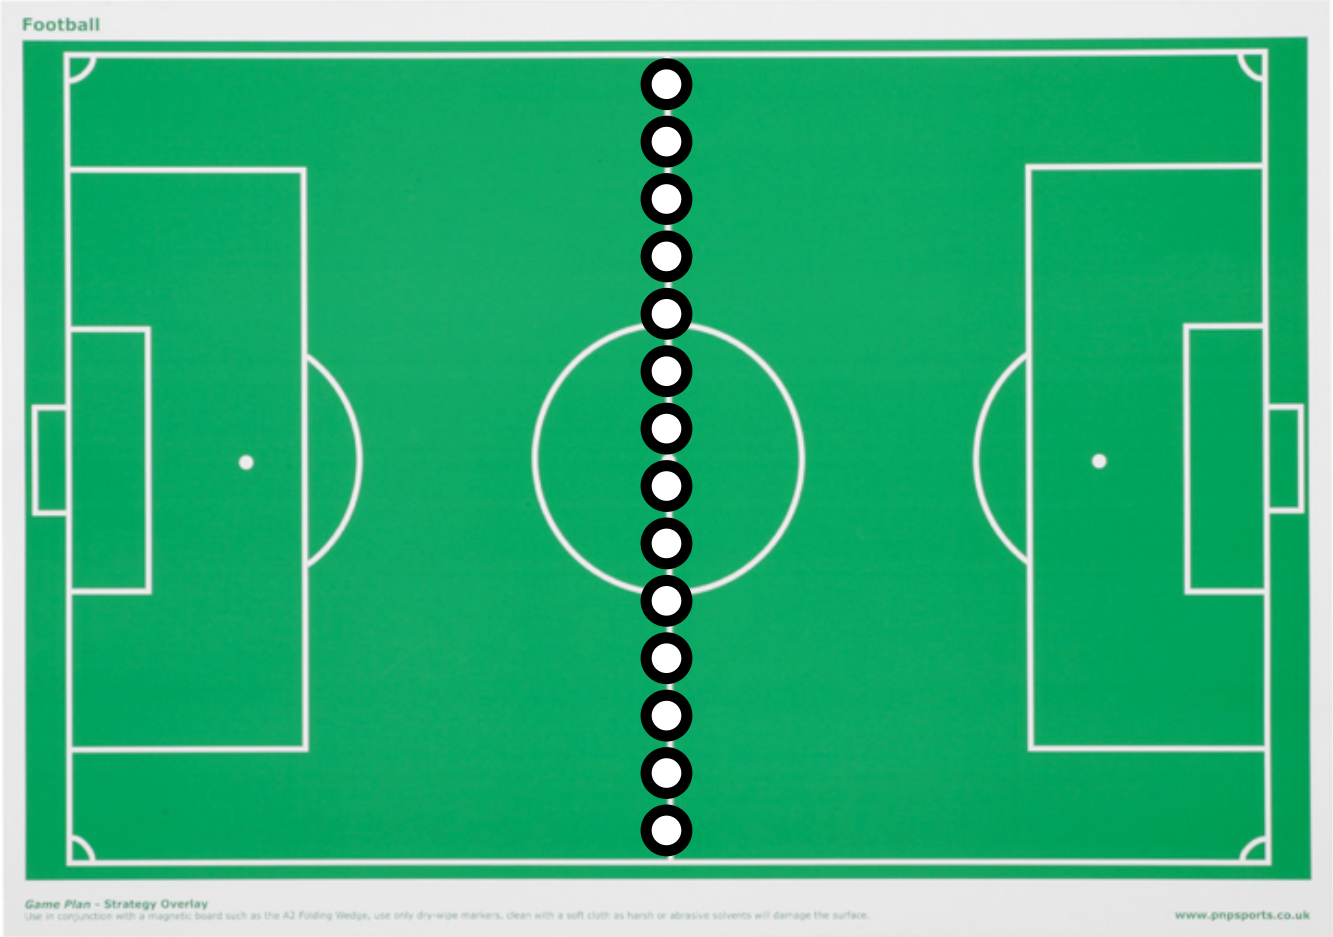
\includegraphics[width=0.9\textwidth]{futbol1}
    \end{center}
\end{frame}

\begin{frame}
    \frametitle{Movimientos en cancha de fútbol}
    \begin{center}
        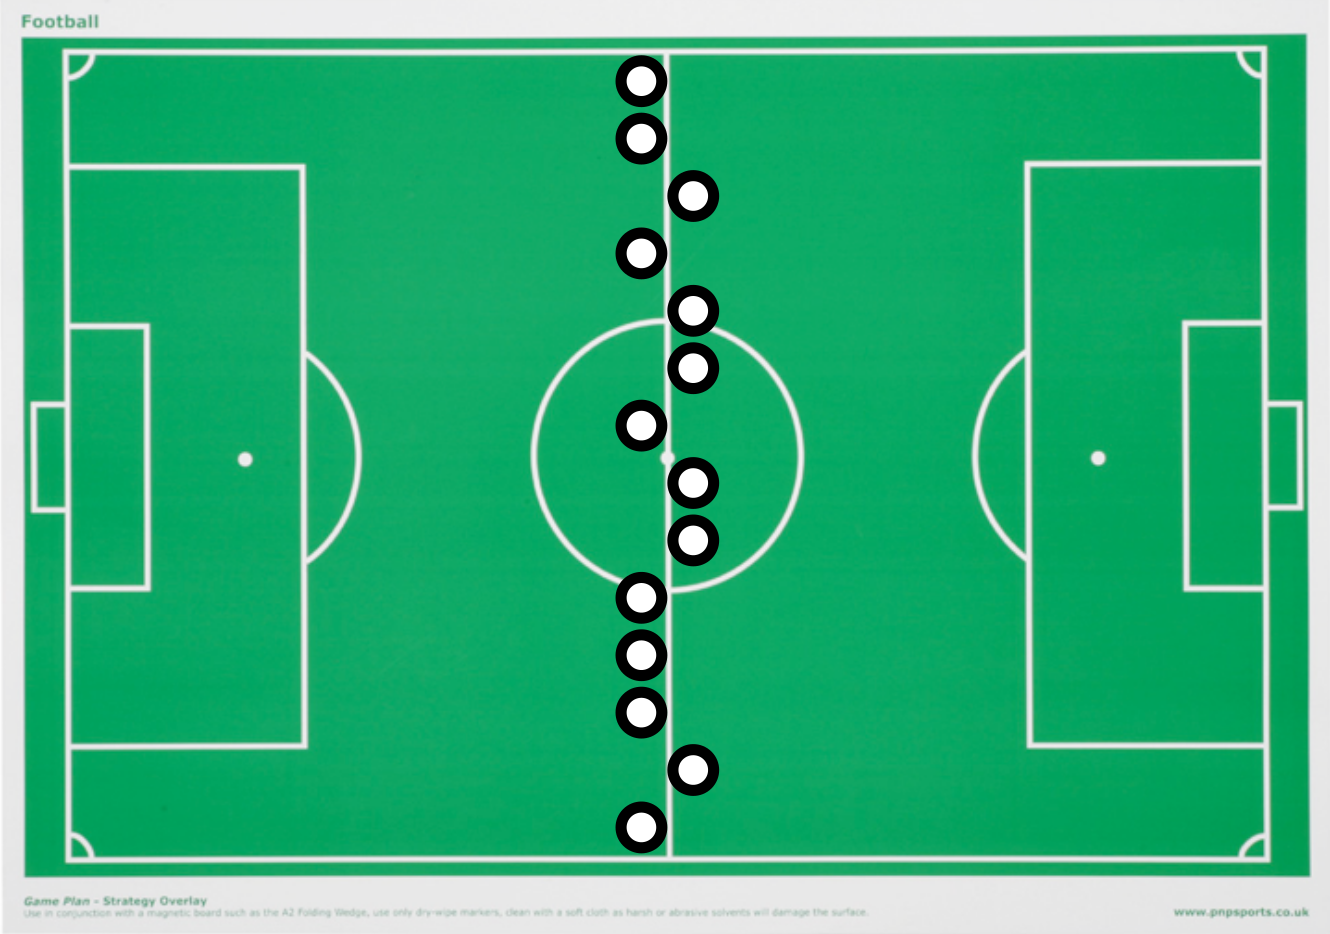
\includegraphics[width=0.9\textwidth]{futbol2}
    \end{center}
\end{frame}

\begin{frame}
    \frametitle{Movimientos en cancha de fútbol}
    \begin{center}
        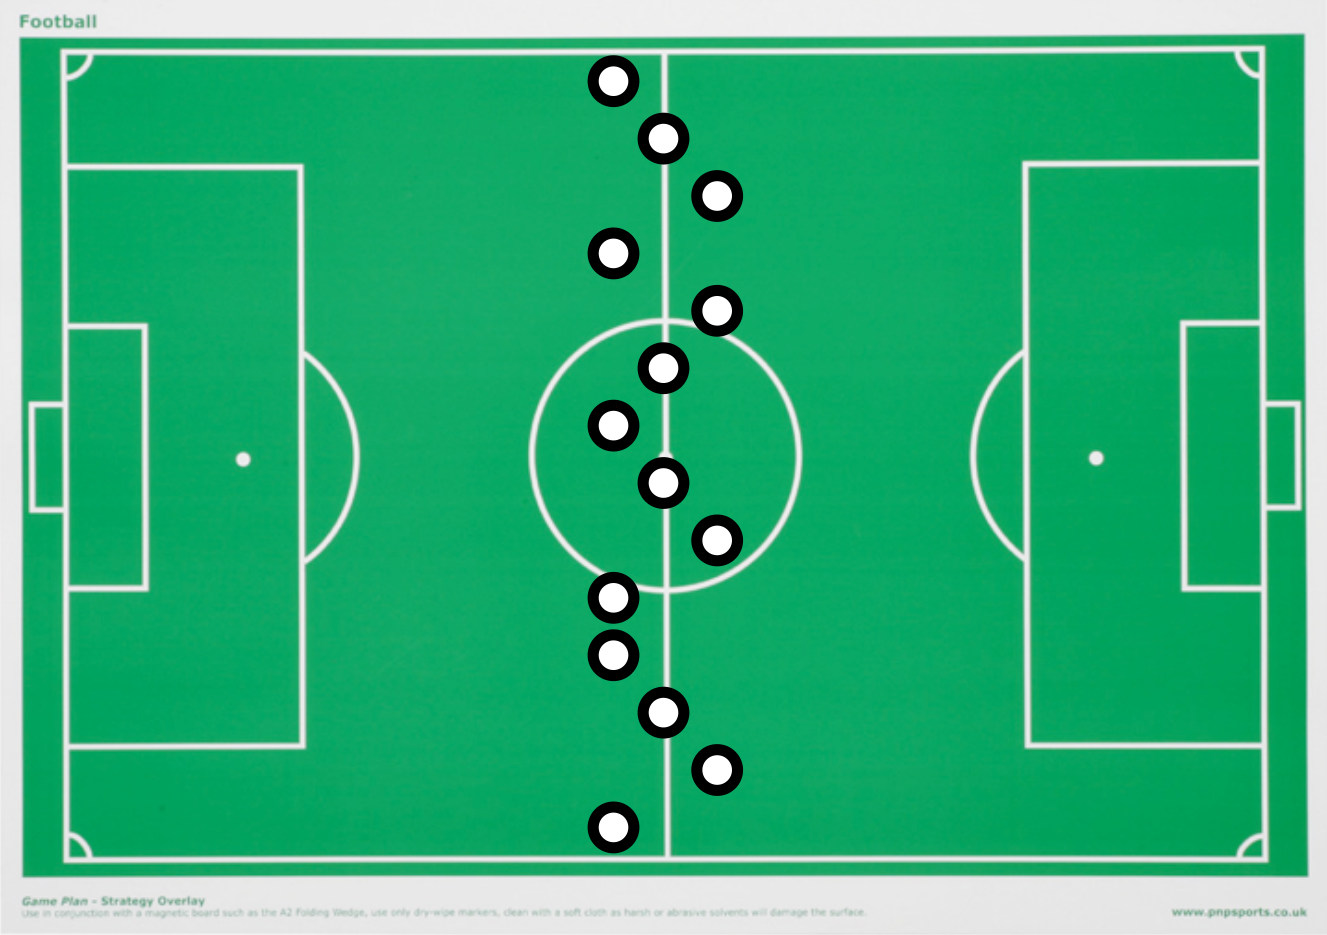
\includegraphics[width=0.9\textwidth]{futbol3}
    \end{center}
\end{frame}

\begin{frame}
    \frametitle{Movimientos en cancha de fútbol}
    \begin{center}
        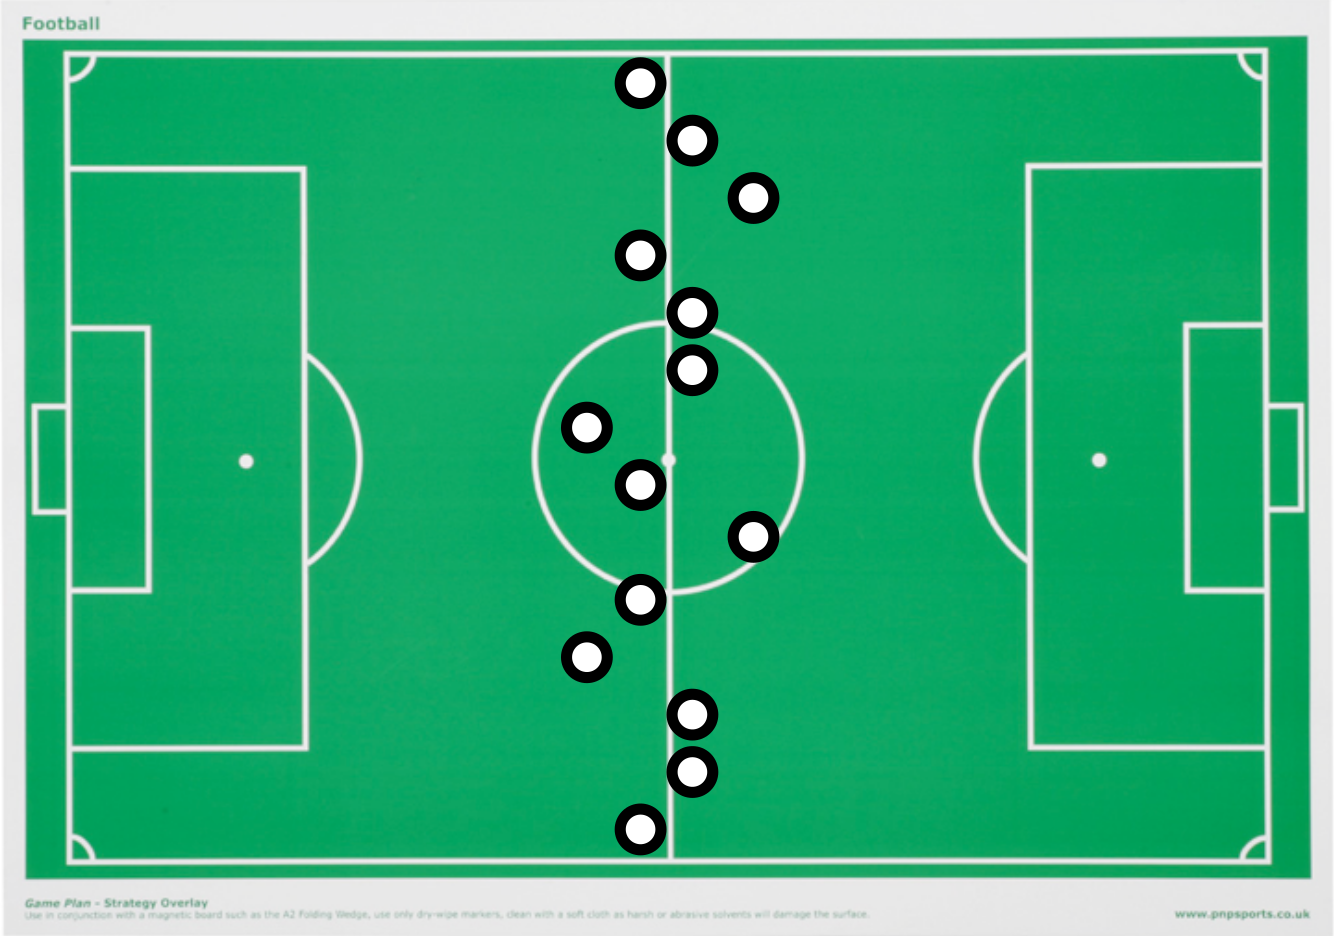
\includegraphics[width=0.9\textwidth]{futbol4}
    \end{center}
\end{frame}
\fi


\iffalse
%%%%%%%% Distribución binomial y distribución normal
\begin{frame}
    \frametitle{Distribución binomial $\binomial{20}{0.6}$ y distribución normal}
    \begin{center}
        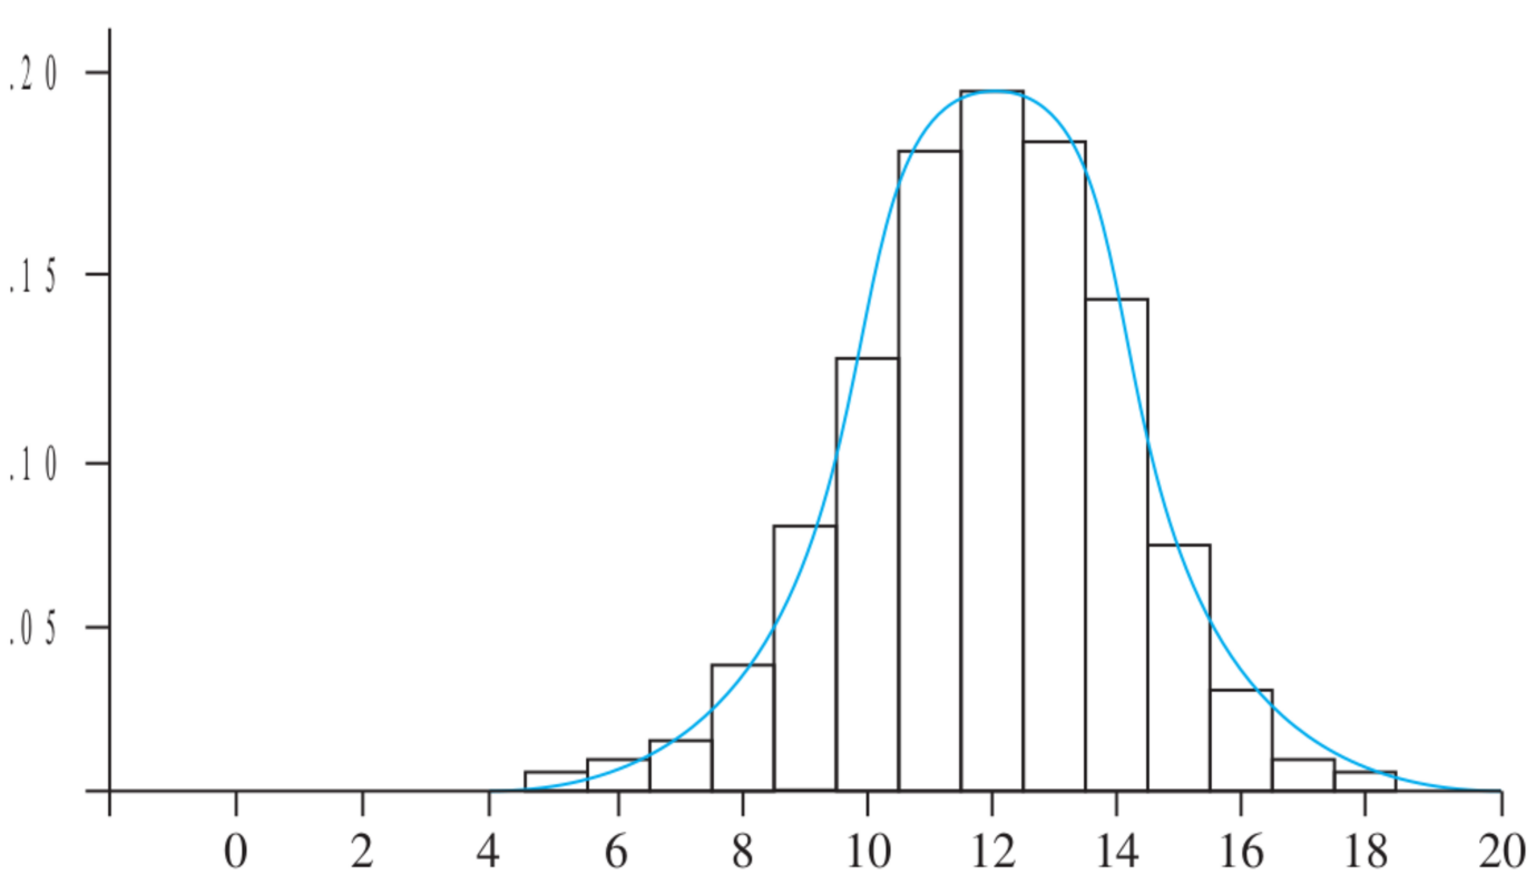
\includegraphics[width=0.9\textwidth]{binomial_normal}
    \end{center}
\end{frame}

\begin{frame}
    \frametitle{Si en vez de $\bernoulli{0.5}$ usamos $\uniform{-1}{1}$}
    \begin{center}
        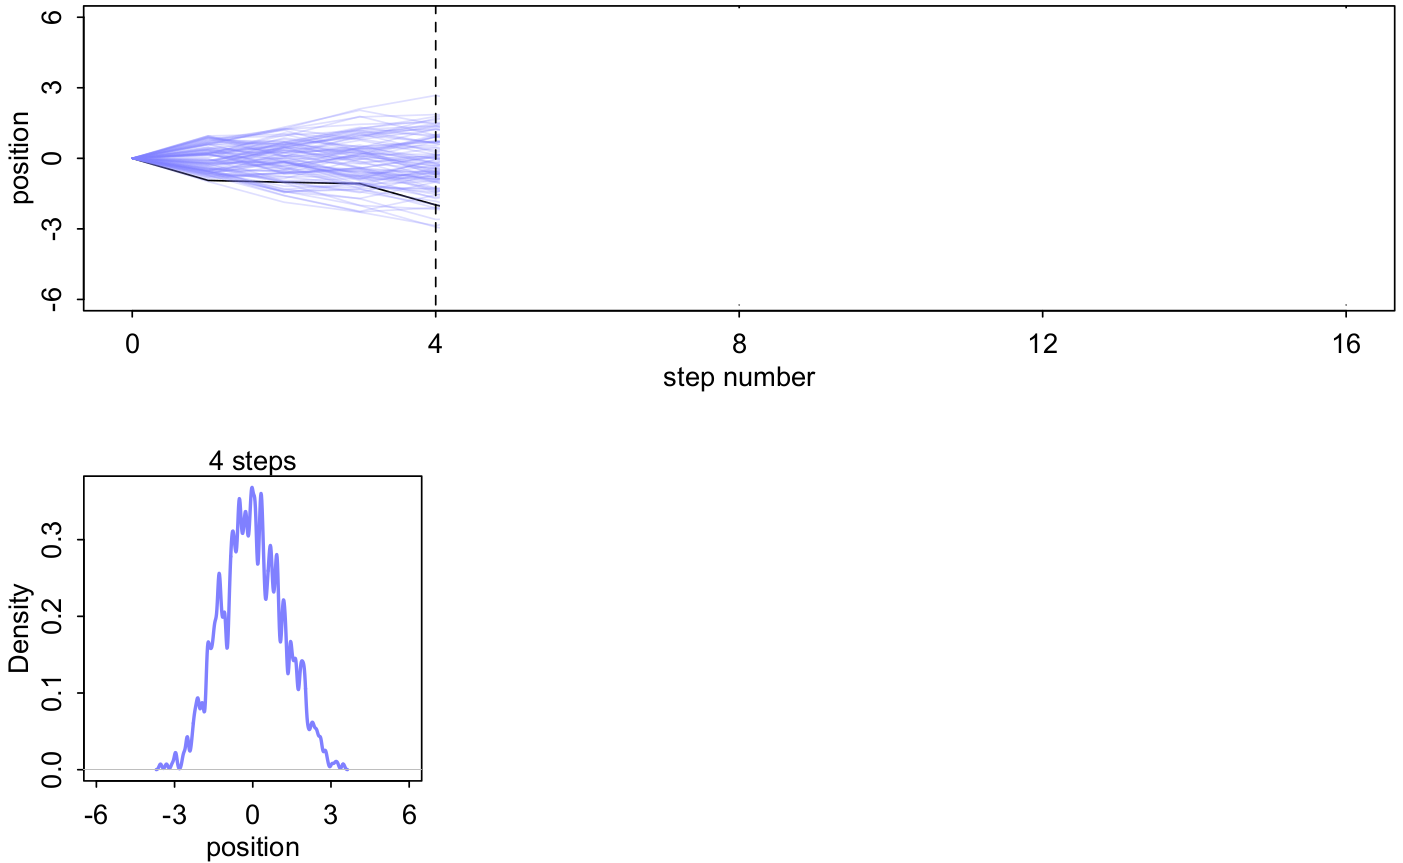
\includegraphics[width=0.9\textwidth]{futbolnormal1}
    \end{center}
\end{frame}

\begin{frame}
    \frametitle{Si en vez de $\bernoulli{0.5}$ usamos $\uniform{-1}{1}$}
    \begin{center}
        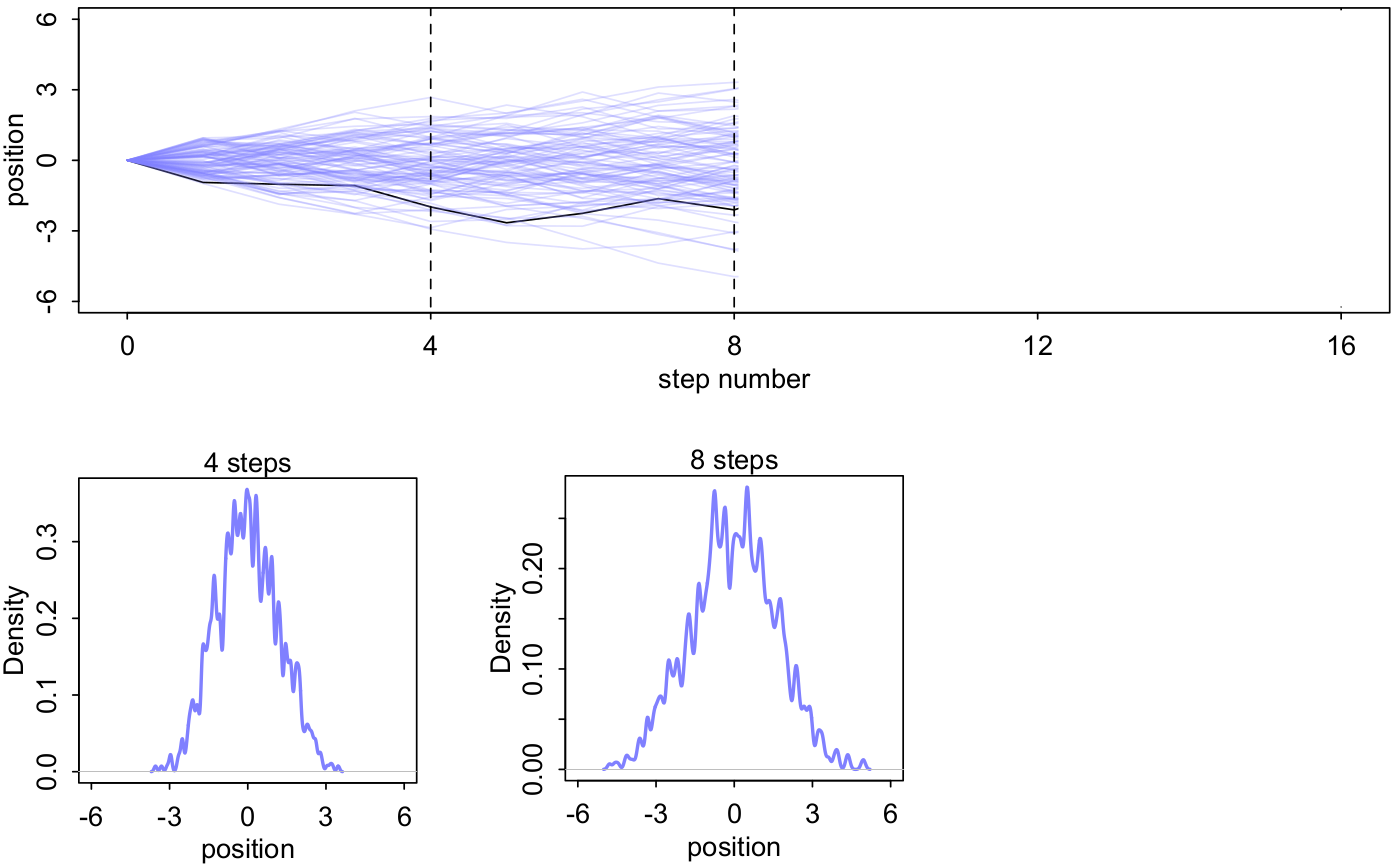
\includegraphics[width=0.9\textwidth]{futbolnormal2}
    \end{center}
\end{frame}

\begin{frame}
    \frametitle{Si en vez de $\bernoulli{0.5}$ usamos $\uniform{-1}{1}$}
    \begin{center}
        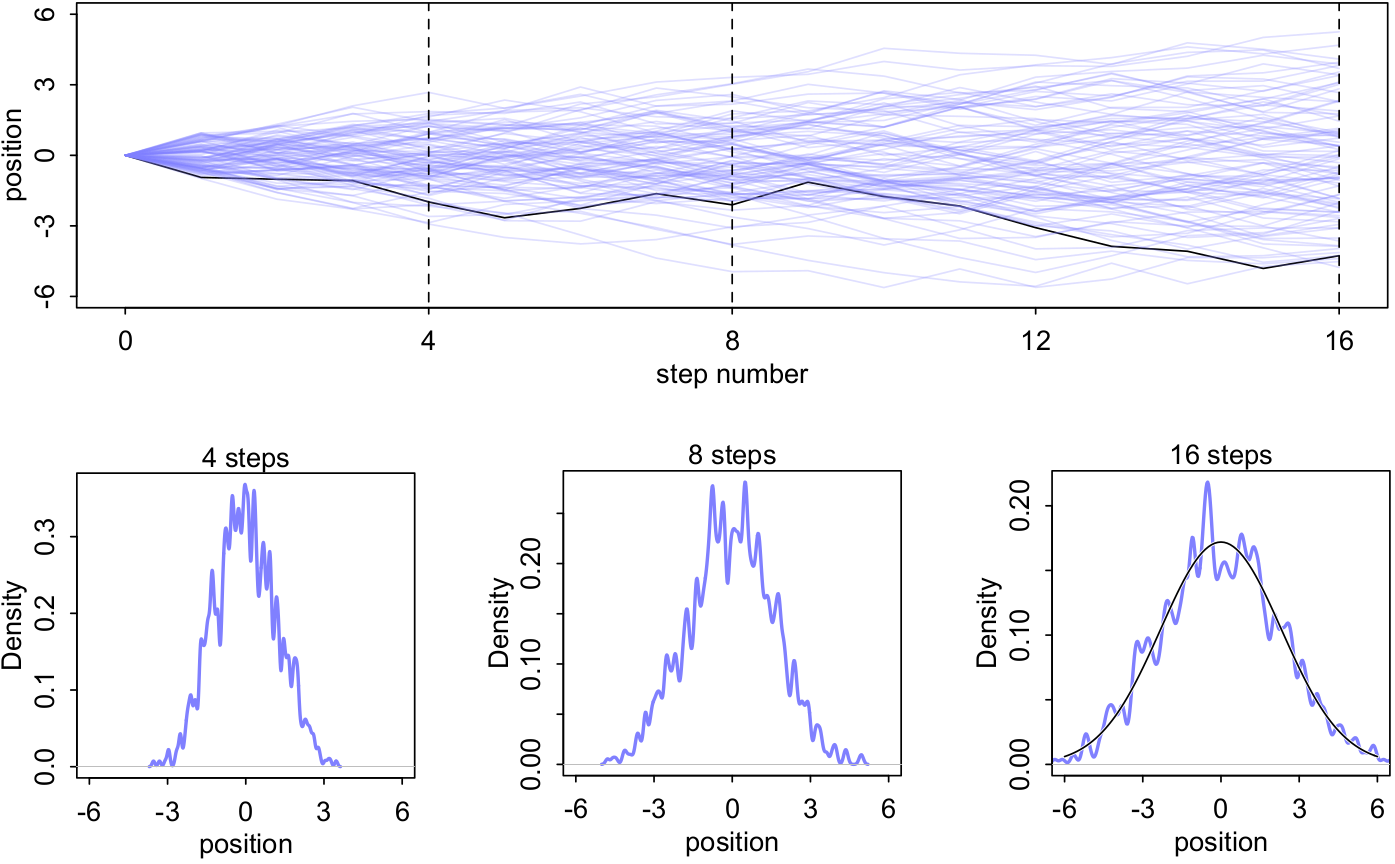
\includegraphics[width=0.9\textwidth]{futbolnormal3}
    \end{center}
\end{frame}

\begin{frame}
    \frametitle{Distribución $\text{Normal} \parens{0, \sigma^{2}} = \normal{0}{\sigma^{2}}$}
    \begin{block}{Converge a}
        \begin{equation*}
            \pdf{x} = \frac{1}{\sqrt{2 \pi \sigma^{2}}} e^{- \frac{x^{2}}{2 \sigma^{2}}} .
        \end{equation*}
    \end{block}
    \begin{center}
        \begin{tabular}{cc}
            \emph{pdf} ($\pdf{x}$) & \emph{cdf} ($\FF{x}$) \\
            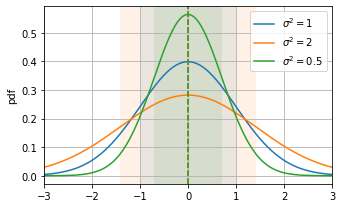
\includegraphics[width=0.42\textwidth]{pdf_normal0} &
            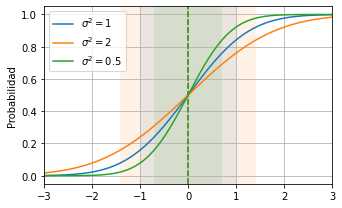
\includegraphics[width=0.42\textwidth]{cdf_normal0}
        \end{tabular}
    \end{center}
    
\end{frame}

%%%%%%%%
\fi

\begin{frame}
    \frametitle{Distribución $\text{Normal} \parens{0, \sigma^{2}} = \normal{0}{\sigma^{2}}$}
        \begin{block}{Propiedades}
        \begin{itemize}
            \item $\expecteddist{X \sim \normal{0}{\sigma^{2}}}{X} = \mu_{X} = 0$.
            \item $\variancedist{X \sim \normal{0}{\sigma^{2}}}{X} = \sigma^{2}_{X} = \sigma^{2}$.
        \end{itemize}
    \end{block}
\end{frame}

\begin{frame}
    \frametitle{Distribución $\text{Normal} \parens{\mu, \sigma^{2}} = \normal{\mu}{\sigma^{2}}$}
    \begin{block}{Definición}
        \begin{equation*}
            \pdf{x} = \frac{1}{\sqrt{2 \pi \sigma^{2}}} e^{- \frac{\parens{x - \mu}^{2}}{2 \sigma^{2}}} .
        \end{equation*}
    \end{block}
    \begin{center}
        \begin{tabular}{cc}
            \emph{pdf} ($\pdf{x}$) & \emph{cdf} ($\FF{x}$) \\
            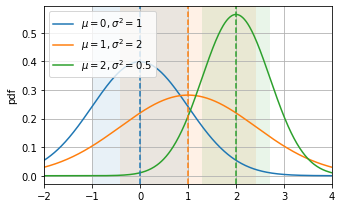
\includegraphics[width=0.42\textwidth]{pdf_normalmu} &
            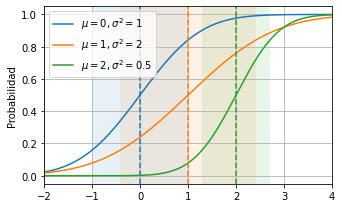
\includegraphics[width=0.42\textwidth]{cdf_normalmu}
        \end{tabular}
    \end{center}
\end{frame}

\begin{frame}
    \frametitle{Distribución $\text{Normal} \parens{\mu, \sigma^{2}} = \normal{\mu}{\sigma^{2}}$}
    \begin{block}{Definición}
        \begin{equation*}
            \pdf{x} = \underbrace{\frac{1}{\sqrt{2 \pi \sigma^{2}}}}_{\text{constante de normalizacion}} e^{- \frac{\parens{x - \mu}^{2}}{2 \sigma^{2}}} .
        \end{equation*}
    \end{block}
    \begin{center}
        \begin{tabular}{cc}
            \emph{pdf} ($\pdf{x}$) & \emph{cdf} ($\FF{x}$) \\
            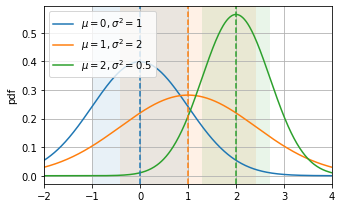
\includegraphics[width=0.42\textwidth]{pdf_normalmu} &
            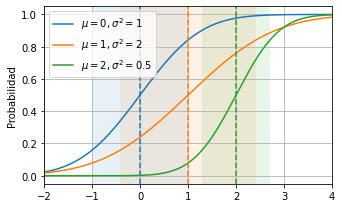
\includegraphics[width=0.42\textwidth]{cdf_normalmu}
        \end{tabular}
    \end{center}
    \begin{block}{Función de distribución acumulada (\emph{cdf})}
        \begin{itemize}
            \item No se puede escribir la \emph{cdf} directamente.
        \end{itemize}
    \end{block}
\end{frame}

\begin{frame}
    \frametitle{Distribución $\text{Normal} \parens{0, 1} = \normal{0}{1}$ estándar}
    \begin{block}{Estandarizando}
        \begin{equation*}
            Z = \frac{X - \mu}{\sigma} \Rightarrow
            \pdf{z} = \frac{1}{\sqrt{2 \pi}} e^{- \frac{z^{2}}{2}} .
        \end{equation*}
        \begin{itemize}
            \item $\mu_{Z} = 0$ y $\sigma^{2}_{Z} = 1$.
        \end{itemize}
    \end{block}
    \begin{block}{Función de distribución acumulada (\emph{cdf}) $\normal{0}{1}$ -- definición}
        \begin{equation*}
            \FF{z} = \Phi \parens{z} = \frac{1}{\sqrt{2 \pi}} \int_{- \infty}^{z} e^{- \frac{t^{2}}{2}} d t .
        \end{equation*}
    \end{block}
    \begin{center}
        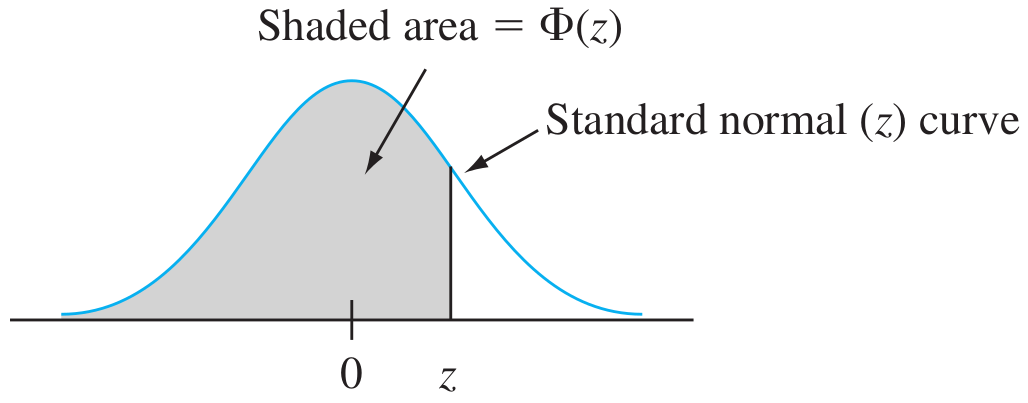
\includegraphics[width=0.5\textwidth]{acumulada_normal}
    \end{center}
\end{frame}

\begin{frame}
    \frametitle{Distribución $\text{Normal} \parens{\mu, \sigma^{2}} = \normal{\mu}{\sigma^{2}}$}
    \begin{block}{Volviendo a $X$: función de distribución acumulada (\emph{cdf}) $\normal{\mu}{\sigma^{2}}$}
        \begin{equation*}
            \FF{x} = \Phi \parens{\frac{x - \mu}{\sigma}} .
        \end{equation*}
    \end{block}
    \begin{center}
        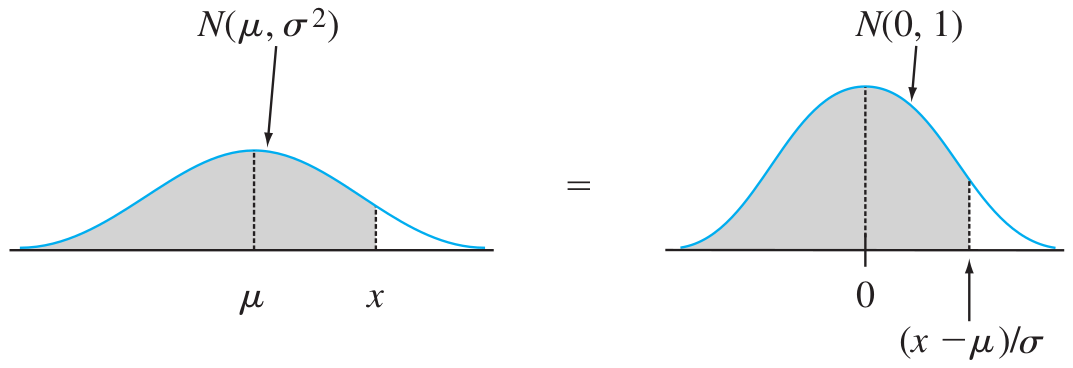
\includegraphics[width=\textwidth]{normal_estandar_otra}
    \end{center}
\end{frame}




\begin{frame}
    \frametitle{Distribución $\text{Normal} \parens{\mu, \sigma^{2}} = \normal{\mu}{\sigma^{2}}$}
    \begin{block}{Probabilidad en intervalo $\sparens{a, b}$}
        \begin{equation*}
            \prob{a \leq X \leq b} = \FF{b} - \FF{a}
            = \Phi \parens{\frac{b - \mu}{\sigma}}
            - \Phi \parens{\frac{a - \mu}{\sigma}} .
        \end{equation*}
    \end{block}
    \begin{center}
        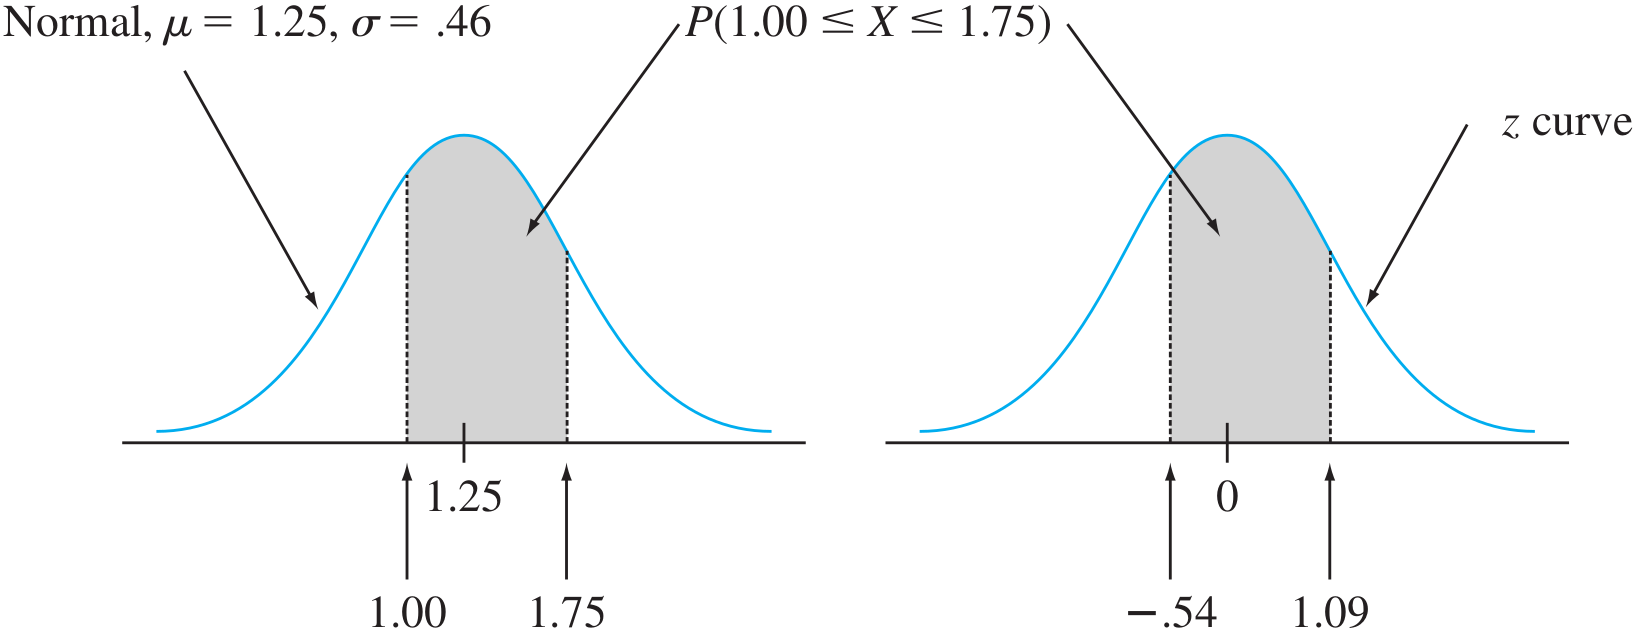
\includegraphics[width=\textwidth]{normal_estandar_otra_2}
    \end{center}
\end{frame}

\begin{frame}
    \frametitle{Distribución $\text{Normal} \parens{\mu, \sigma^{2}} = \normal{\mu}{\sigma^{2}}$}
    \begin{center}
        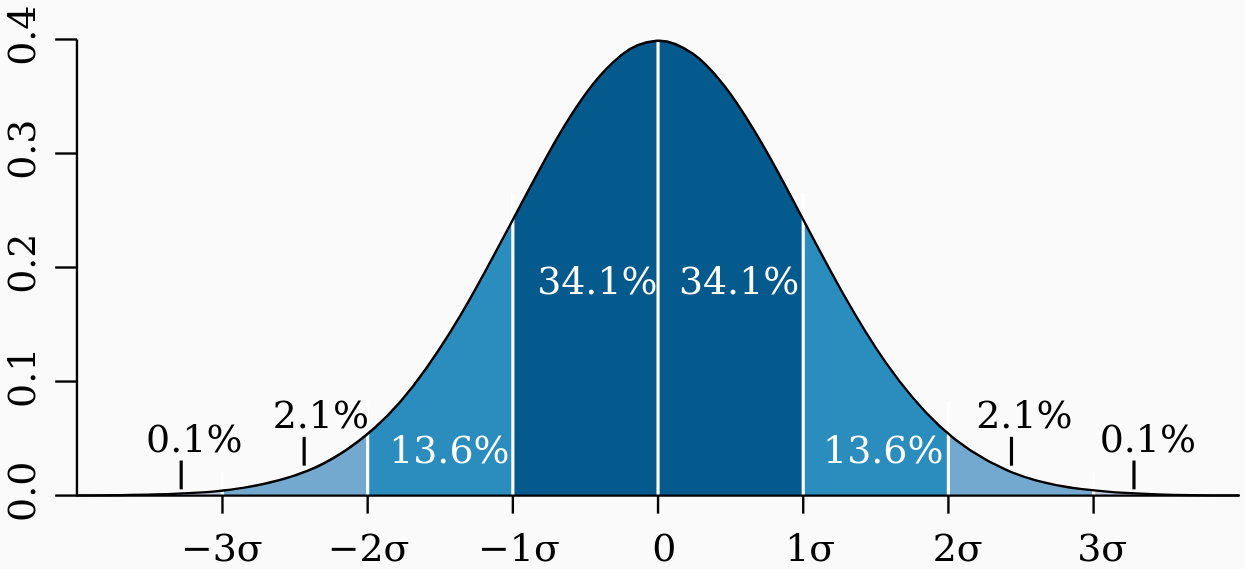
\includegraphics[width=\textwidth]{standard_normal_percentages}
    \end{center}
\end{frame}

\begin{frame}
    \frametitle{Distribución normal}
    \begin{exampleblock}{Ejemplo: altura personas en Chile}
        \begin{itemize}
            \item Se ha determinado que la altura media de las mujeres es de $159.4$ cm.
            \item Se ha determinado que la altura media de los hombres es de $171.8$ cm.
            \item Suponiendo que la altura se distribuye como una normal:
                \begin{itemize}
                    \item ¿Es un hombre que mide $165$ cm. bajo?
                    \item ¿Es una mujer que mide $165$ cm. alta?
                \end{itemize}
        \end{itemize}
    \end{exampleblock}
    \begin{block}{Respuesta}
        \begin{itemize}
            \item ¡Depende de la desviación estándar / varianza!
        \end{itemize}
    \end{block}
\end{frame}

\begin{frame}
    \frametitle{Distribución normal}
    \begin{center}
        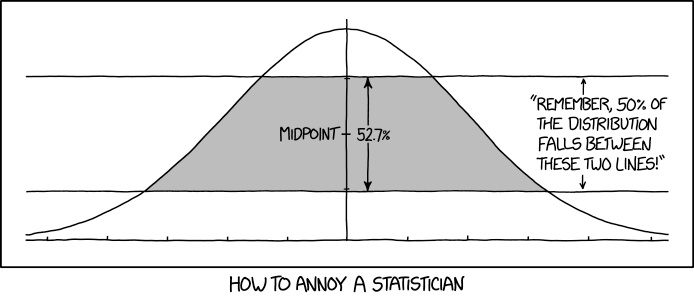
\includegraphics[width=\textwidth]{xkcd_normal_distribution}
    \end{center}
\end{frame}

\begin{frame}
    \frametitle{Distribución $\text{Normal} \parens{\mu, \sigma^{2}} = \normal{\mu}{\sigma^{2}}$}
    \begin{center}
        \begin{tabular}{cc}
            \emph{pdf} ($\pdf{x}$) & \emph{cdf} ($\FF{x}$) \\
            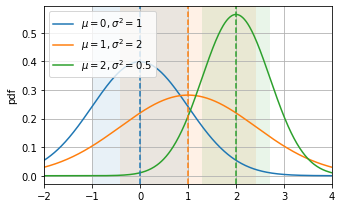
\includegraphics[width=0.36\textwidth]{pdf_normalmu} &
            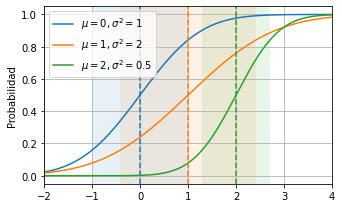
\includegraphics[width=0.36\textwidth]{cdf_normalmu}
        \end{tabular}
    \end{center}
    \begin{block}{Tal vez ayuda para recordar}
        \begin{equation*}
            \ln \parens{\pdf{x}} = - \frac{1}{2} \ln \parens{2 \pi \sigma^{2}} - \frac{\parens{x - \mu}^{2}}{2 \sigma^{2}} .
        \end{equation*}
    \end{block}
    \begin{center}
        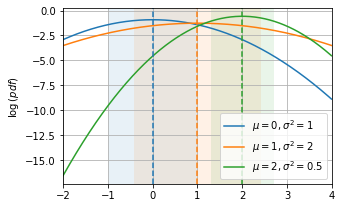
\includegraphics[width=0.32\textwidth]{pdflog_normalmu}
    \end{center}
\end{frame}

\begin{frame}
    \frametitle{¿Por qué usar distribución $\normal{\mu}{\sigma^{2}}$?}
    \begin{block}{}
        \begin{itemize}
            \item Termodinámica: distribución tiene la mayor entropía, sujeto a $\mu$ y $\sigma^{2}$.
            \item Igualmente, distribución con menos información además de $\mu$ y $\sigma^{2}$.
            \item La suma de distribuciones converge a una distribución normal.
            \item Logaritmo de producto de distribuciones converge a una normal.
        \end{itemize}
    \end{block}
    \begin{center}
        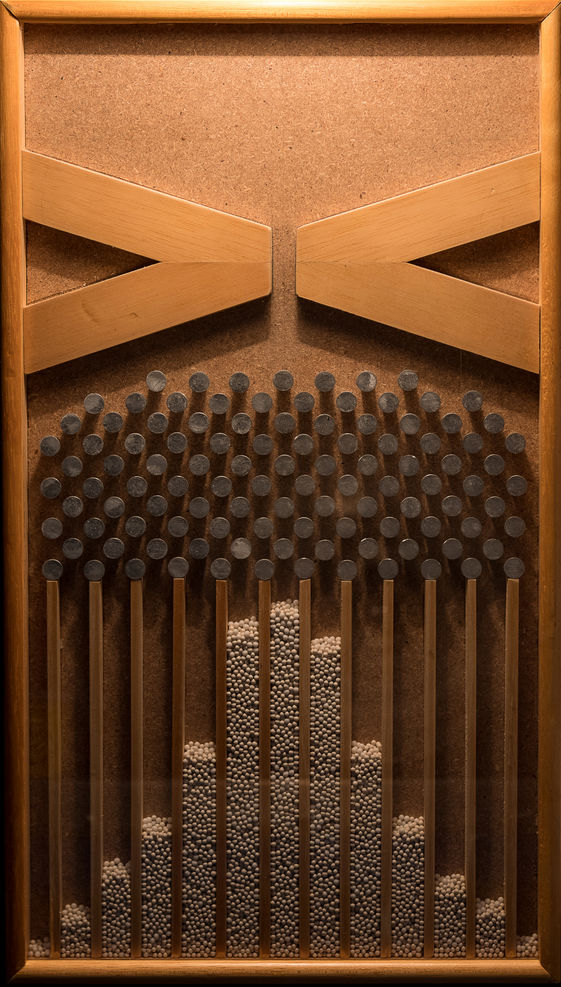
\includegraphics[height=0.6\textheight]{galton}
    \end{center}
\end{frame}

\begin{frame}
    \frametitle{Sobre constante de normalización}
    \begin{block}{Recordar}
        \begin{equation*}
            \pdf{x} = \underbrace{\frac{1}{\sqrt{2 \pi \sigma^{2}}}}_{\text{constante de normalizacion}} e^{- \frac{\parens{x - \mu}^{2}}{2 \sigma^{2}}} .
        \end{equation*}
    \end{block}
    \end{frame}

\begin{frame}
    \frametitle{Sobre constante de normalización}

    \begin{block}{En general}
        \begin{itemize}
            \item Muchas veces se define la ``forma'' de una distribución.
            \item Ejemplos:
                \begin{itemize}
                    \item $\pdf{x} \propto 1$.
                    \item $\pdf{x} \propto e^{- x^{2}}$.
                    \item $\pdf{x} \propto e^{- x}$, con $x \geq 0$.
                    \item $\pdf{x} \propto e^{- \vparens{x}}$.
                \end{itemize}
            \item Luego se calcula la constante de normalización para que sea una distribución de probabilidad:
                \begin{equation*}
                    \int_{- \infty}^{\infty} \pdf{x} d x = 1.
                \end{equation*}
        \end{itemize}
    \end{block}
\end{frame}

%%%%%%%&&&



\begin{frame}
    \frametitle{Sobre constante de normalización}
    \begin{exampleblock}{Ejemplo}
        \begin{equation*}
            \pdf{x} \propto e^{- \lambda x} , \text{ con } x \geq 0 , \lambda > 0 .
        \end{equation*}
    \end{exampleblock}
    \begin{block}{Desarrollo}
        \begin{equation*}
            \int_{0}^{\infty} \pdf{x} d x = \int_{0}^{\infty} c e^{- \lambda x} d x
            = - c \evalparens{\frac{e^{- \lambda x}}{\lambda}}_{x = 0}^{\infty}
            %= \parens{- \frac{e^{- \lambda \infty}}{\lambda} + \frac{e^{0}}{\lambda}}
            = \frac{c}{\lambda} = 1
            \Rightarrow c = \lambda .
        \end{equation*}
    \end{block}
    \begin{block}{Entonces}
        \begin{equation*}
            \pdf{x} = \lambda e^{- \lambda x} , \text{ con } x \geq 0 , \lambda > 0 .
        \end{equation*}
    \end{block}
\end{frame}



\begin{frame}
    \frametitle{Sobre constante de normalización}
    \begin{exampleblock}{Ejemplo}
        \begin{equation*}
            \pdf{x} \propto e^{- \frac{\vparens{x - \mu}}{b} } , \text{ con } b > 0 .
        \end{equation*}
    \end{exampleblock}
    \begin{block}{Desarrollo}
        \begin{multline*}
            \int_{- \infty}^{\infty} \pdf{x} d x
            = \int_{- \infty}^{\mu} c e^{- \frac{\vparens{x - \mu}}{b}} d x + \int_{\mu}^{\infty} c e^{- \frac{\vparens{x - \mu}}{b}} d x
            \\
            = \int_{- \infty}^{\mu} c e^{\frac{x - \mu}{b}} d x + \int_{\mu}^{\infty} c e^{- \frac{x - \mu}{b}} d x
            = c \evalparens{b e^{\frac{x - \mu}{b}}}_{x = - \infty}^{\mu}
            - c \evalparens{b e^{- \frac{x - \mu}{b}}}_{x = \mu}^{\infty}
            \\
            = 2 b c = 1
            \Rightarrow c = \frac{1}{2 b} .
        \end{multline*}
    \end{block}
    \begin{block}{Entonces}
        \begin{equation*}
            \pdf{x} = \frac{1}{2 b} e^{- \frac{\vparens{x - \mu}}{b}} , \text{ con } b > 0 .
        \end{equation*}
    \end{block}
\end{frame}



\begin{frame}
    \frametitle{Distribución $\laplace{\mu}{b}$}
    \begin{block}{Definición}
        \begin{equation*}
            \pdf{x} = \frac{1}{2 b} e^{- \frac{\vparens{x - \mu}}{b}} , \text{ con } b > 0 .
        \end{equation*}
    \end{block}
    \begin{center}
        \begin{tabular}{cc}
            \emph{pdf} ($\pdf{x}$) & \emph{cdf} ($\FF{x}$) \\
            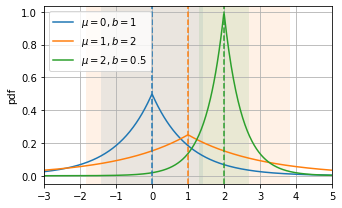
\includegraphics[width=0.42\textwidth]{pdf_laplace} &
            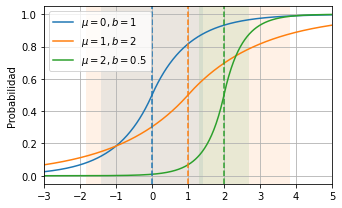
\includegraphics[width=0.42\textwidth]{cdf_laplace}
        \end{tabular}
    \end{center}
    \begin{block}{Propiedades}
        \begin{itemize}
            \item $\expecteddist{X \sim \laplace{\mu}{b}}{X} = \mu_{X} = \mu$.
            \item $\variancedist{X \sim \laplace{\mu}{b}}{X} = \sigma^{2}_{X} = 2 b^{2}$.
        \end{itemize}
    \end{block}
\end{frame}

\begin{frame}
    \frametitle{¿Por qué usar distribución $\normal{\mu}{\sigma^{2}}$?}
    \begin{block}{No acotada}
        \begin{itemize}
            \item ¿Y si los datos son solo positivos?
            \item ¿Y si los datos están acotados entre dos valores?
        \end{itemize}
    \end{block}
\end{frame}



\begin{frame}
    \frametitle{Distribución $\text{Gamma} \parens{\alpha, \beta} = \gammadist{\alpha}{\beta}$}
    \begin{block}{Definición}
        \begin{equation*}
            \pdf{x} = \underbrace{\frac{\beta^{\alpha}}{\gammafunc{\alpha}}}_{\text{normalizacion}} x^{\alpha - 1} e^{- \beta x} ,
            \text{ con } x \in \parens{0, + \infty} .
        \end{equation*}
    \end{block}
    \begin{center}
        \begin{tabular}{cc}
            \emph{pdf} ($\pdf{x}$) & \emph{cdf} ($\FF{x}$) \\
            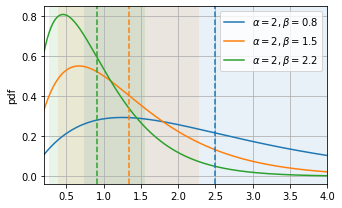
\includegraphics[width=0.35\textwidth]{pdf_gamma0} &
            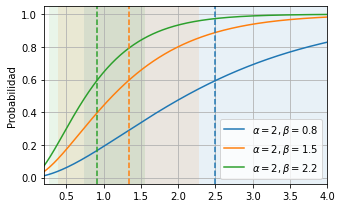
\includegraphics[width=0.35\textwidth]{cdf_gamma0} \\
            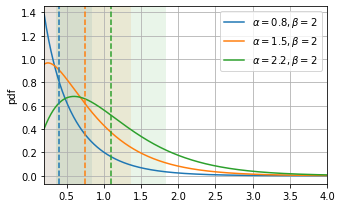
\includegraphics[width=0.35\textwidth]{pdf_gamma1} &
            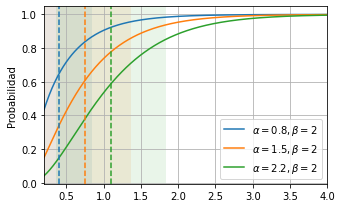
\includegraphics[width=0.35\textwidth]{cdf_gamma1}
        \end{tabular}
    \end{center}
\end{frame}

\begin{frame}
    \frametitle{Distribución $\text{Gamma} \parens{\alpha, \beta} = \gammadist{\alpha}{\beta}$}
    \begin{block}{Definición}
        \begin{equation*}
            \pdf{x} = \underbrace{\frac{\beta^{\alpha}}{\gammafunc{\alpha}}}_{\text{normalizacion}} x^{\alpha - 1} e^{- \beta x} ,
            \text{ con } x \in \parens{0, + \infty} .
        \end{equation*}
    \end{block}
    \begin{block}{Nota}
        \begin{equation*}
            \gammafunc{\alpha} = \int_{0}^{+ \infty} x^{\alpha - 1} e^{- x} d x .
        \end{equation*}
    \end{block}
    \begin{block}{Propiedades}
        \begin{itemize}
            \item $\expecteddist{X \sim \gammadist{\alpha}{\beta}}{X} = \mu_{X} = \frac{\alpha}{\beta}$.
            \item $\variancedist{X \sim \gammadist{\alpha}{\beta}}{X} = \sigma^{2}_{X} = \frac{\alpha}{\beta^{2}}$.
        \end{itemize}
    \end{block}
\end{frame}

\begin{frame}
    \frametitle{Distribución $\betadist{\alpha}{\beta}$}
    \begin{block}{Definición}
        \begin{equation*}
            \pdf{x} = \underbrace{\frac{\gammafunc{\alpha + \beta}}{\gammafunc{\alpha} \gammafunc{\beta}}}_{\text{normalizacion}} x^{\alpha - 1} \parens{1 - x}^{\beta- 1} ,
            \text{ con } x \in \sparens{0, 1} .
        \end{equation*}
    \end{block}
    \begin{center}
        \begin{tabular}{cc}
            \emph{pdf} ($\pdf{x}$) & \emph{cdf} ($\FF{x}$) \\
            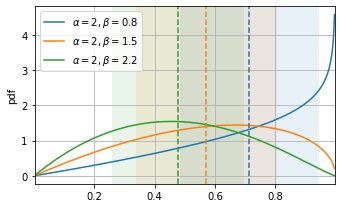
\includegraphics[width=0.35\textwidth]{pdf_beta0} &
            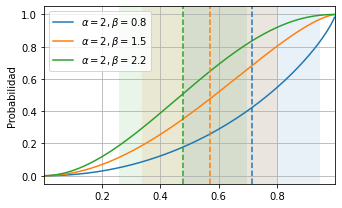
\includegraphics[width=0.35\textwidth]{cdf_beta0} \\
            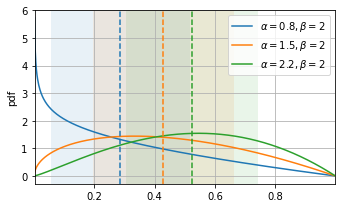
\includegraphics[width=0.35\textwidth]{pdf_beta1} &
            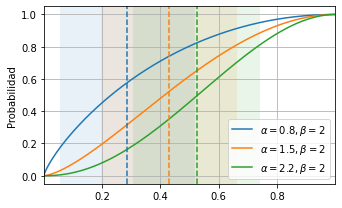
\includegraphics[width=0.35\textwidth]{cdf_beta1}
        \end{tabular}
    \end{center}
\end{frame}

\begin{frame}
    \frametitle{Distribución $\betadist{\alpha}{\beta}$}
    \begin{block}{Definición}
        \begin{equation*}
            \pdf{x} = \underbrace{\frac{1}{\betafunc{\alpha}{\beta}}}_{\text{normalizacion}} x^{\alpha - 1} \parens{1 - x}^{\beta- 1} ,
            \text{ con } x \in \sparens{0, 1} .
        \end{equation*}
    \end{block}
    \begin{block}{Definición}
        \begin{equation*}
            \betafunc{\alpha}{\beta} =
            \int_{0}^{1} x^{\alpha - 1} \parens{1 - x}^{\beta - 1} dx =
            \frac{\gammafunc{\alpha} \gammafunc{\beta}}{\gammafunc{\alpha + \beta}} .
        \end{equation*}
    \end{block}
    \begin{block}{Propiedades}
        \begin{itemize}
            \item $\expecteddist{X \sim \betadist{\alpha}{\beta}}{X} = \mu_{X} = \frac{\alpha}{\alpha + \beta}$.
            \item $\variancedist{X \sim \betadist{\alpha}{\beta}}{X} = \sigma^{2}_{X} = \frac{\alpha \beta}{\parens{\alpha + \beta}^{2} \parens{\alpha + \beta + 1}}$.
        \end{itemize}
    \end{block}
\end{frame}

\begin{frame}
    \frametitle{¿Cómo construir distribuciones?}
    \begin{block}{Supuestos}
        \begin{itemize}
            \item $X$ variable aleatoria continua.
            \item $f : \reals \rightarrow \reals$ función invertible y monótona.
            \item $Y = \ff{X}$ nueva variable aleatoria.
        \end{itemize}
    \end{block}
    \begin{center}
        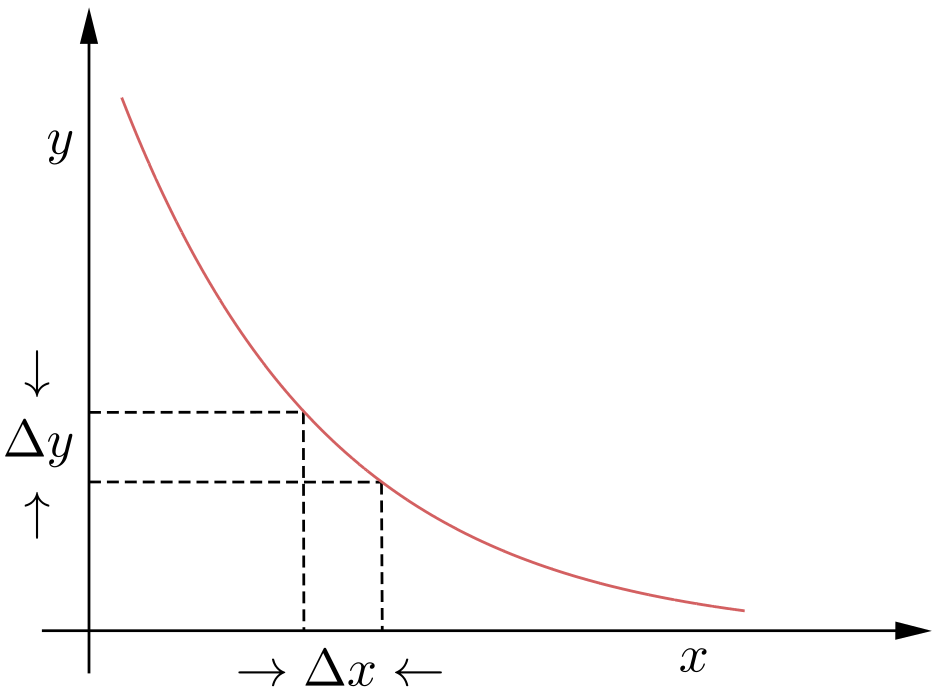
\includegraphics[width=0.45\textwidth]{transformacion}
    \end{center}
\end{frame}

\begin{frame}
    \frametitle{¿Cómo construir distribuciones?}
    \begin{block}{Se tiene que}
        \begin{equation*}
            \pFF{Y}{y} = \prob{Y \leq y} = \prob{X \geq f^{-1} \parens{y}} = 1 - \pFF{X}{f^{-1} \parens{y}} .
        \end{equation*}
        \begin{itemize}
            \item Derivando con respecto a $y$:
        \end{itemize}
        \begin{equation*}
            \ppdf{Y}{y} = - \ppdf{X}{f^{-1} \parens{y}} \sparens{f^{-1}}' \parens{y}
            = - \frac{\ppdf{X}{f^{-1} \parens{y}}}{f' \parens{f^{-1} \parens{y}}} .
        \end{equation*}
    \end{block}
    \begin{center}
        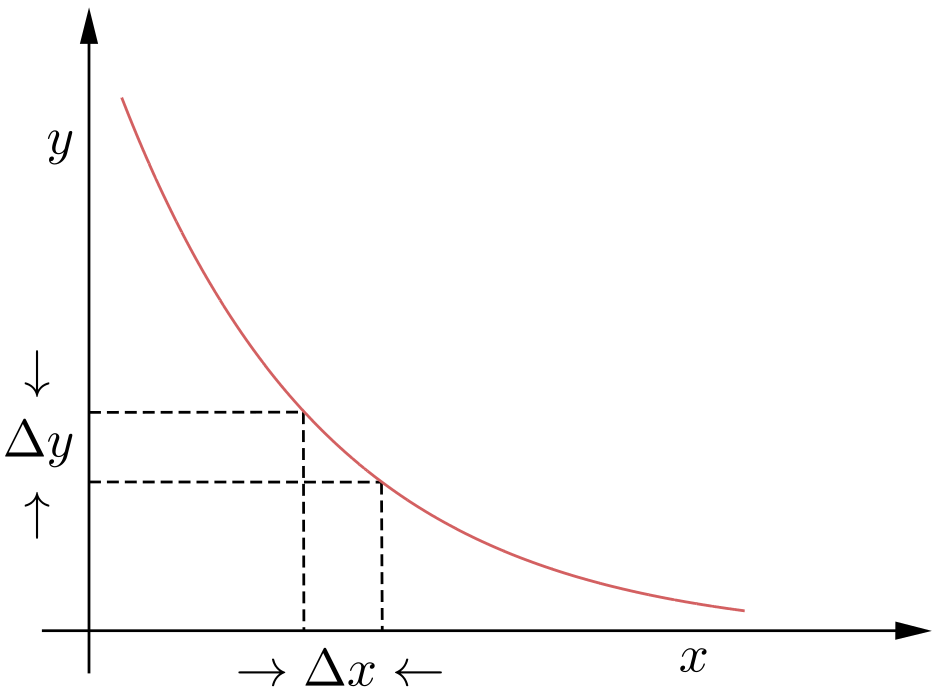
\includegraphics[width=0.45\textwidth]{transformacion}
    \end{center}
\end{frame}

\begin{frame}
    \frametitle{¿Cómo construir distribuciones?}
    \begin{block}{Dos casos}
        \begin{itemize}
            \item Caso $y$ monótona decreciente:
                \begin{equation*}
                    \ppdf{Y}{y} = - \frac{\ppdf{X}{f^{-1} \parens{y}}}{f' \parens{f^{-1} \parens{y}}} .
                \end{equation*}
            \item Caso $y$ monótona creciente:
                \begin{multline*}
                    \pFF{Y}{y} = \prob{Y \leq y} = \prob{X \leq f^{-1} \parens{y}} = \pFF{X}{f^{-1} \parens{y}} \\
                    \Rightarrow
                    \ppdf{Y}{y} = \frac{\ppdf{X}{f^{-1} \parens{y}}}{f' \parens{f^{-1} \parens{y}}} .
                \end{multline*}
        \end{itemize}
    \end{block}
    \begin{center}
        \includegraphics[width=0.37\textwidth]{transformacion}
    \end{center}
\end{frame}


\begin{frame}
    \frametitle{¿Cómo construir distribuciones?}
    \begin{block}{En general}
        \begin{equation*}
            \ppdf{Y}{y} = \frac{\ppdf{X}{f^{-1} \parens{y}}}{\vparens{f' \parens{f^{-1} \parens{y}}}} .
        \end{equation*}
    \end{block}
    \begin{center}
        \includegraphics[width=0.45\textwidth]{transformacion}
    \end{center}
\end{frame}

\begin{frame}
    \frametitle{Transformaciones}
    \begin{exampleblock}{Ejemplo}
        \begin{itemize}
            \item Si $X \sim \normal{0}{1}$, ¿cómo se distribuye $Y = \mu + \sigma X$?
        \end{itemize}
    \end{exampleblock}
    \begin{block}{Desarrollo}
        \begin{itemize}
            \item $\ff{x} = \mu + \sigma x$.
            \item $f' \parens{x} = \sigma$.
            \item $f^{-1} \parens{y} = \frac{y - \mu}{\sigma}$.
            \item Luego,
                \begin{equation*}
                    \ppdf{Y}{y}
                    = \frac{\ppdf{X}{f^{-1} \parens{y}}}{\vparens{f' \parens{f^{-1} \parens{y}}}}
                    = \frac{1}{\sqrt{2 \pi}} e^{- \frac{\parens{\frac{y - \mu}{\sigma}}^{2}}{2}} \frac{1}{\vparens{\sigma}}
                    = \frac{1}{\sqrt{2 \pi \sigma^{2}}} e^{- \frac{\parens{y - \mu}^{2}}{2 \sigma^{2}}} .
                \end{equation*}
        \end{itemize}
    \end{block}
    \begin{block}{Conclusión}
        \begin{itemize}
            \item $Y \sim \normal{\mu}{\sigma}$.
        \end{itemize}
    \end{block}
\end{frame}

\begin{frame}
    \frametitle{Transformaciones}
    \begin{exampleblock}{Ejemplo}
        \begin{itemize}
            \item Si $X \sim \normal{\mu}{\sigma}$, ¿cómo se distribuye $Y = e^{X}$?
        \end{itemize}
    \end{exampleblock}
    \begin{block}{Desarrollo}
        \begin{itemize}
            \item $\ff{x} = e^{x}$.
            \item $f' \parens{x} = e^{x}$.
            \item $f^{-1} \parens{y} = \ln \parens{y}$.
            \item Luego,
                \begin{multline*}
                    \ppdf{Y}{y}
                    = \frac{\ppdf{X}{f^{-1} \parens{y}}}{\vparens{f' \parens{f^{-1} \parens{y}}}}
                    = \frac{1}{\sqrt{2 \pi \sigma^{2}}} e^{- \frac{\parens{\ln \parens{y} - \mu}^{2}}{2 \sigma^{2}}} \frac{1}{e^{\ln \parens{y}}}
                    \\
                    \Rightarrow
                    \ppdf{Y}{y}
                    = \frac{1}{y \sqrt{2 \pi \sigma^{2}}} e^{- \frac{\parens{\ln \parens{y} - \mu}^{2}}{2 \sigma^{2}}} , \text{ con } y \in \parens{0, + \infty} .
                \end{multline*}
        \end{itemize}
    \end{block}
    
\end{frame}

\begin{frame}
    \frametitle{Transformaciones}
       \begin{block}{Conclusión}
        \begin{itemize}
            \item $Y$ sigue distribución llamada Log-normal ($Y \sim \text{Lognormal} \parens{\mu, \sigma}$).
        \end{itemize}
    \end{block}
\end{frame}


\begin{frame}
    \frametitle{Transformaciones}
    \begin{exampleblock}{Ejemplo}
        \begin{itemize}
            \item Si $X \sim \uniform{0}{1}$, ¿cómo se distribuye $Y = \ln \parens{X}$?
        \end{itemize}
    \end{exampleblock}
    \begin{center}
        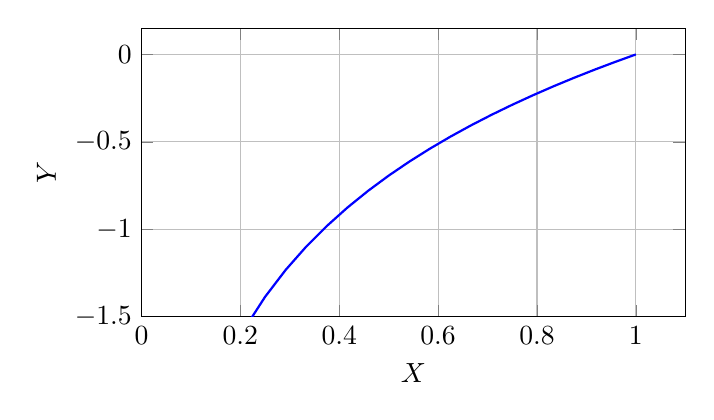
\begin{tikzpicture}
            \begin{axis}[
                %footnotesize,
                %clip=false,
                domain=0:1,
                ymin=-1.5,
                %ymax=0,
                xmin=0,
                %max=1,
                ylabel=$Y$,
                xlabel=$X$,
                height=0.7\textwidth/1.618,
                width=0.7\textwidth,
                %xtick distance=1,
                %axis lines=middle,
                grid=major,
                no markers,
                ]
                \addplot+[thick] {ln(x)};
            \end{axis}
        \end{tikzpicture}
    \end{center}
\end{frame}

\begin{frame}
    \frametitle{Transformaciones}
    \begin{exampleblock}{Ejemplo}
        \begin{itemize}
            \item Si $X \sim \uniform{0}{1}$, ¿cómo se distribuye $Y = \ln \parens{X}$?
        \end{itemize}
    \end{exampleblock}
    \begin{block}{Desarrollo}
        \begin{itemize}
            \item $\ff{x} = \ln \parens{x}$.
            \item $f' \parens{x} = \frac{1}{x}$.
            \item $f^{-1} \parens{y} = e^{y}$.
            \item Luego,
                \begin{equation*}
                    \ppdf{Y}{y}
                    = \frac{\ppdf{X}{f^{-1} \parens{y}}}{\vparens{f' \parens{f^{-1} \parens{y}}}}
                    = 1 \frac{1}{\frac{1}{e^{y}}}
                    = e^{y} , \text{ con } y \in \left ( - \infty , 0 \right ] .
                \end{equation*}
        \end{itemize}
    \end{block}
\end{frame}

\begin{frame}
    \frametitle{Transformaciones -- ¿y si $f$ no es monótona?}
    \begin{exampleblock}{Por ejemplo}
        \begin{itemize}
            \item $X \sim \normal{0}{1}$.
            \item $Y = X^{2}$.
        \end{itemize}
    \end{exampleblock}
    \begin{block}{Separar parte negativa y positiva}
        \begin{multline*}
            \pFF{Y}{y} = \prob{Y \leq y} = \prob{X^{2} \leq y}
            = \prob{- \sqrt{y} \leq X \leq \sqrt{y}}
            \\
            = \prob{X \leq \sqrt{y}} - \prob{X \leq - \sqrt{y}}
            = \pFF{X}{\sqrt{y}} - \pFF{X}{- \sqrt{y}}
            \\
            \Rightarrow
            \ppdf{Y}{y} =
            \frac{\ppdf{X}{\sqrt{y}}}{2 \sqrt{y}} - \frac{\ppdf{X}{- \sqrt{y}}}{- 2 \sqrt{y}}
            = \frac{1}{2 \sqrt{y}} \parens{\ppdf{X}{\sqrt{y}} + \ppdf{X}{- \sqrt{y}}}
            \\
            \Rightarrow
            \ppdf{Y}{y}
            = \frac{1}{\sqrt{2 \pi y}} e^{-\frac{y}{2}} ,
            \text{ con } y \in \left [ 0 , + \infty \right ) .
        \end{multline*}
    \end{block}
    \begin{block}{Conclusión}
        \begin{itemize}
            \item $Y$ sigue distribución llamada ji al cuadrado ($Y \sim \chidist{1}$).
        \end{itemize}
    \end{block}
\end{frame}

\begin{frame}
    \frametitle{Transformaciones -- ¿y si $f$ no es monótona?}
    \begin{exampleblock}{Ejemplo}
        \begin{itemize}
            \item Si $X \sim \uniform{0}{1}$, ¿cómo se distribuye $Y = \sin \parens{\pi X}$?
        \end{itemize}
    \end{exampleblock}
    \begin{center}
        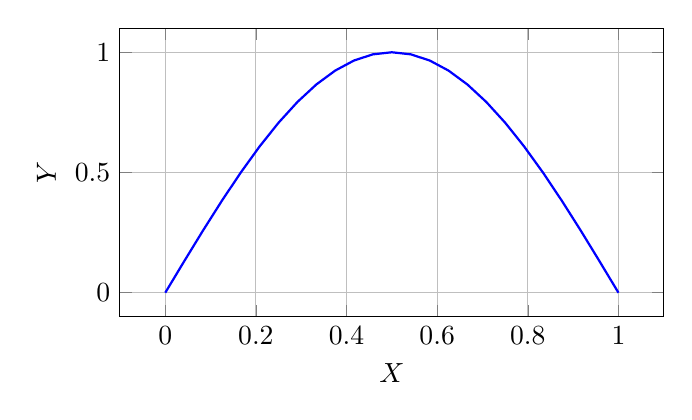
\begin{tikzpicture}
            \begin{axis}[
                %footnotesize,
                %clip=false,
                domain=0:1,
                %ymin=-1.5,
                %ymax=0,
                %xmin=0,
                %max=1,
                ylabel=$Y$,
                xlabel=$X$,
                height=0.7\textwidth/1.618,
                width=0.7\textwidth,
                %xtick distance=1,
                %axis lines=middle,
                grid=major,
                no markers,
                ]
                \addplot+[thick] {sin(180 * x)};
            \end{axis}
        \end{tikzpicture}
    \end{center}
\end{frame}

\begin{frame}
    \frametitle{Transformaciones -- ¿y si $f$ no es monótona?}
    \begin{block}{Desarrollo}
        \begin{itemize}
            \item Si $X \sim \uniform{0}{1}$, ¿cómo se distribuye $Y = \sin \parens{\pi X}$?
        \end{itemize}
        \begin{multline*}
            \pFF{Y}{y} = \prob{Y \leq y}
            = \prob{\sin \parens{\pi X} \leq y}
            \\
            = \prob{\pi X \leq \arcsin \parens{y}} + \prob{\pi X > \pi - \arcsin \parens{y}}
            \\
            = \prob{\pi X \leq \arcsin \parens{y}} + 1 - \prob{\pi X \leq \pi - \arcsin \parens{y}}
            \\
            = \frac{1}{\pi} \arcsin \parens{y} + 1 - \frac{1}{\pi} \parens{\pi - \arcsin \parens{y}}
            = \frac{2}{\pi} \arcsin \parens{y}
            \\
            \Rightarrow
            \ppdf{Y}{y} = \frac{2}{\pi \sqrt{1 - y^{2}}} , \text{ con } y \in \parens{0 , 1}
        \end{multline*}
    \end{block}
    \begin{center}
        \begin{tikzpicture}
            \begin{axis}[
                footnotesize,
                %clip=false,
                domain=0:1,
                ymax=1.5,
                %ymax=0,
                %xmin=0,
                %max=1,
                ylabel=$\ppdf{Y}{y}$,
                xlabel=$y$,
                height=0.32\textheight,
                width=0.32\textheight*1.618,
                %xtick distance=1,
                %axis lines=middle,
                grid=major,
                no markers,
                ]
                \addplot+[thick] {2 / 3.14159 / sqrt(1 - x * x)};
            \end{axis}
        \end{tikzpicture}
    \end{center}
\end{frame}

\begin{frame}
    % \frametitle{Transformaciones}
    \begin{center}
        \includegraphics[height=0.99\textheight]{distribution_zoo}
    \end{center}
\end{frame}

\begin{frame}
    \frametitle{Extensión a varias variables aleatorias discretas}
    \begin{block}{Probabilidad conjunta}
        \begin{equation*}
            \prob{X = x, Y = y} = \pff{X, Y}{x, y} .
        \end{equation*}
        \begin{equation*}
            \prob{X \leq x, Y \leq y} = \pFF{X, Y}{x, y}
            = \sum_{x' = - \infty}^{x} \sum_{y' = - \infty}^{y} \pff{X, Y}{x', y'} .
        \end{equation*}
    \end{block}
    \begin{center}
        \small
        \begin{tabular}{c|c|cccc|c}
            & & \multicolumn{4}{c|}{$X$} & \\
            \hline
            & $\pff{X, Y}{x, y}$ & 1 & 2 & 3 & 4 & $\pff{Y}{y}$ \\
            \hline
            & 1 & 0.1 & 0.33 & 0.15 & 0.04 & 0.62 \\
            $Y$ & 2 & 0 & 0.03 & 0.2 & 0.02 & 0.25 \\
            & 3 & 0 & 0 & 0.05 & 0.08 & 0.13 \\
            \hline
            & $\pff{X}{x}$ & 0.1 & 0.36 & 0.4 & 0.14 &
        \end{tabular}
    \end{center}
    \begin{block}{Probabilidad marginal}
        \begin{equation*}
            \prob{X = x} = \pff{X}{x} = \sum_{y = - \infty}^{+ \infty} \pff{X, Y}{x, y}
            = \sum_{y = - \infty}^{+ \infty} \prob{X = x, Y = y} .
        \end{equation*}
    \end{block}
\end{frame}

\begin{frame}
    \frametitle{Extensión a varias variables aleatorias continuas}
    \begin{block}{Probabilidad conjunta}
        \begin{equation*}
            \prob{X \leq x, Y \leq y} = \pFF{X, Y}{x, y}
            = \int_{- \infty}^{x} \int_{- \infty}^{y} \ppdf{X, Y}{x', y'} d y' d x' .
        \end{equation*}
    \end{block}
    \begin{center}
        \includegraphics[width=0.31\textwidth]{marginales_continua}
    \end{center}
    \begin{block}{Función de densidad de probabilidad (\emph{pdf}) marginal}
        \begin{equation*}
            \ppdf{X}{x} = \int_{- \infty}^{\infty} \ppdf{X, Y}{x, y} d y .
        \end{equation*}
    \end{block}
\end{frame}

\begin{frame}
    \frametitle{Probabilidades y variables aleatorias}
    \begin{block}{Eventos}
        \begin{itemize}
            \item Caso discreto:
                \begin{equation*}
                    \prob{\parens{X, Y} \in A} = \sum_{\parens{x, y} \in A} \pff{X, Y}{x, y} .
                \end{equation*}
            \item Caso continuo:
                \begin{equation*}
                    \prob{\parens{X, Y} \in A} = \iint_{\parens{x, y} \in A} \ppdf{X, Y}{x, y} d x d y .
                \end{equation*}
        \end{itemize}
    \end{block}
    \begin{center}
        \includegraphics[width=0.65\textwidth]{eventos_va}
    \end{center}
\end{frame}

\begin{frame}
    \frametitle{Probabilidades y variables aleatorias}
    \begin{block}{Recuerdo de definiciones}
        \begin{itemize}
            \item Probabilidad condicional:
                \begin{equation*}
                    \prob{A \mid B} = \frac{\prob{A, B}}{\prob{B}} .
                \end{equation*}
            \item Independencia:
                \begin{equation*}
                    \prob{A, B} = \prob{A} \prob{B} .
                \end{equation*}
        \end{itemize}
    \end{block}
    \begin{center}
        \small
        \begin{tabular}{c|c|cccc|c}
            & & \multicolumn{4}{c|}{$X$} & \\
            \hline
            & $\pff{X, Y}{x, y}$ & 1 & 2 & 3 & 4 & $\pff{Y}{y}$ \\
            \hline
            & 1 & 0.1 & 0.33 & 0.15 & 0.04 & 0.62 \\
            $Y$ & 2 & 0 & 0.03 & 0.2 & 0.02 & 0.25 \\
            & 3 & 0 & 0 & 0.05 & 0.08 & 0.13 \\
            \hline
            & $\pff{X}{x}$ & 0.1 & 0.36 & 0.4 & 0.14 &
        \end{tabular}
    \end{center}
   
\end{frame}

\begin{frame}
    \frametitle{Probabilidades y variables aleatorias}
    
    \begin{center}
        \begin{tabular}{c|c}
            $Y$ & $\pff{Y \mid X = 3}{y}$ \\
            \hline
            1 & 0.375 \\
            2 & 0.5 \\
            3 & 0.125
        \end{tabular}
    \end{center}
\end{frame}


\begin{frame}
    \frametitle{Extensión a varias variables aleatorias discretas}
    \begin{block}{Probabilidad condicional}
        \begin{equation*}
            \pff{X \mid Y}{x \mid y} = \frac{\pff{X, Y}{x, y}}{\pff{Y}{y}} .
        \end{equation*}
    \end{block}
    \begin{block}{Independencia}
        \begin{equation*}
            \pff{X, Y}{x, y} = \pff{X}{x} \pff{Y}{y} .
        \end{equation*}
    \end{block}
    \begin{block}{Regla del producto}
        \begin{equation*}
            \pff{X, Y}{x, y} = \pff{X \mid Y}{x \mid y} \pff{Y}{y} .
        \end{equation*}
    \end{block}
    \begin{block}{Teorema de Bayes}
        \begin{equation*}
            \pff{Y \mid X}{y \mid x} = \frac{\pff{X \mid Y}{x \mid y} \pff{Y}{y}}{\pff{X}{x}} .
        \end{equation*}
    \end{block}
\end{frame}

\begin{frame}
    \frametitle{Extensión a varias variables aleatorias continuas}
    \begin{block}{Probabilidad condicional}
        \begin{equation*}
            \ppdf{X \mid Y}{x \mid y} = \frac{\ppdf{X, Y}{x, y}}{\ppdf{Y}{y}} .
        \end{equation*}
    \end{block}
    \begin{block}{Independencia}
        \begin{equation*}
            \ppdf{X, Y}{x, y} = \ppdf{X}{x} \ppdf{Y}{y} .
        \end{equation*}
    \end{block}
    \begin{block}{Regla del producto}
        \begin{equation*}
            \ppdf{X, Y}{x, y} = \ppdf{X \mid Y}{x \mid y} \ppdf{Y}{y} .
        \end{equation*}
    \end{block}
    \begin{block}{Teorema de Bayes}
        \begin{equation*}
            \ppdf{Y \mid X}{y \mid x} = \frac{\ppdf{X \mid Y}{x \mid y} \ppdf{Y}{y}}{\ppdf{X}{x}} .
        \end{equation*}
    \end{block}
\end{frame}


\begin{frame}
    \frametitle{Extensión a varias variables aleatorias}
    \begin{center}
        \small
        \begin{tabular}{c|c|cccc|c}
            & & \multicolumn{4}{c|}{$X$} & \\
            \hline
            & $\pff{X, Y}{x, y}$ & 1 & 2 & 3 & 4 & $\pff{Y}{y}$ \\
            \hline
            & 1 & 0.1 & 0.33 & 0.15 & 0.04 & 0.62 \\
            $Y$ & 2 & 0 & 0.03 & 0.2 & 0.02 & 0.25 \\
            & 3 & 0 & 0 & 0.05 & 0.08 & 0.13 \\
            \hline
            & $\pff{X}{x}$ & 0.1 & 0.36 & 0.4 & 0.14 &
        \end{tabular}
    \end{center}
    \begin{block}{Probabilidad marginal}
        \begin{equation*}
            \prob{X = x} = \pff{X}{x} = \sum_{y = - \infty}^{+ \infty} \pff{X, Y}{x, y}
            = \sum_{y = - \infty}^{+ \infty} \pff{X \mid Y}{x \mid y} \pff{Y}{y} .
        \end{equation*}
    \end{block}
    \begin{block}{Función de densidad de probabilidad (\emph{pdf}) marginal}
        \begin{equation*}
            \ppdf{X}{x} = \int_{- \infty}^{\infty} \ppdf{X, Y}{x, y} d y
            = \int_{- \infty}^{\infty} \ppdf{X \mid Y}{x \mid y} \ppdf{Y}{y} d y .
        \end{equation*}
    \end{block}
\end{frame}

\begin{frame}
    \frametitle{Extensión a varias variables aleatorias}
    \begin{block}{Valor esperado / esperanza}
        \begin{itemize}
            \item Caso discreto:
                \begin{equation*}
                    \expecteddist{X, Y}{X, Y} = \expecteddist{X, Y}{\parens{X, Y}} = \sum_{x = - \infty}^{+ \infty} \sum_{y = - \infty}^{+ \infty} \parens{x , y} \pff{X, Y}{x , y} .
                \end{equation*}
            \item Caso continuo:
                \begin{equation*}
                    \expecteddist{X, Y}{X, Y} = \expecteddist{X, Y}{\parens{X, Y}} = \int_{- \infty}^{+ \infty} \int_{- \infty}^{+ \infty} \parens{x , y} \ppdf{X, Y}{x , y} d y d x .
                \end{equation*}
        \end{itemize}
    \end{block}
    \begin{center}
        \includegraphics[width=0.31\textwidth]{marginales_continua}
    \end{center}
\end{frame}

\begin{frame}
    \frametitle{Probabilidad marginal... ¡De nuevo!}
    \begin{block}{Probabilidad marginal}
        \begin{equation*}
            \prob{X = x} = \pff{X}{x}
            %= \sum_{y = - \infty}^{+ \infty} \pff{X, Y}{x, y}
            = \sum_{y = - \infty}^{+ \infty} \pff{X \mid Y}{x \mid y} \pff{Y}{y}
            = \expecteddist{Y}{\pff{X \mid Y}{x \mid y}} .
        \end{equation*}
    \end{block}
    \begin{block}{Función de densidad de probabilidad (\emph{pdf}) marginal}
        \begin{equation*}
            \ppdf{X}{x}
            % = \int_{- \infty}^{\infty} \ppdf{X, Y}{x, y} d y
            = \int_{- \infty}^{\infty} \ppdf{X \mid Y}{x \mid y} \ppdf{Y}{y} d y
            = \expecteddist{Y}{\ppdf{X \mid Y}{x \mid y}} .
        \end{equation*}
    \end{block}
    \begin{center}
        \includegraphics[width=0.31\textwidth]{marginales_continua}
    \end{center}
\end{frame}

\begin{frame}
    \frametitle{Extensión a varias variables aleatorias}
    \begin{block}{Covarianza y varianza}
        \begin{multline*}
            \cov{X, Y} = \expecteddist{X , Y}{\parens{X - \expecteddist{X}{X}} \parens{Y - \expecteddist{Y}{Y}}}
            \\
            = \expecteddist{X, Y}{X Y} - \expecteddist{X}{X} \expecteddist{Y}{Y} .
        \end{multline*}
        \begin{multline*}
            \variance{X} = \cov{X, X} = \expecteddist{X}{\parens{X - \expecteddist{X}{X}} \parens{X - \expecteddist{X}{X}}}
            \\
            = \expecteddist{X}{X^{2}} - \expecteddist{X}{X}^{2} .
        \end{multline*}
    \end{block}
    \begin{center}
        \includegraphics[width=0.4\textwidth]{covar_func}
        \includegraphics[width=0.5\textwidth]{correlacion_va}
    \end{center}
\end{frame}

\begin{frame}
    \frametitle{Extensión a varias variables aleatorias}
    \begin{block}{Correlación}
        \begin{equation*}
            \corr{X , Y} = \frac{\cov{X , Y}}{\sqrt{\variance{X} \variance{Y}}} \in \sparens{-1 , 1} .
        \end{equation*}
    \end{block}
    \begin{center}
        \includegraphics[width=0.4\textwidth]{covar_func}
        \includegraphics[width=0.5\textwidth]{correlacion_va}
    \end{center}
\end{frame}


\begin{frame}
    \frametitle{Correlación}
    \begin{center}
        \includegraphics[width=0.9\textwidth]{correlaciones_1}
        \includegraphics[width=0.9\textwidth]{correlaciones_2}
    \end{center}
\end{frame}

\begin{frame}
    \frametitle{Correlación}
    \begin{block}{Ejemplo}
        \begin{itemize}
            \item $X$ variable aleatoria con media $0$ ($\expecteddist{X}{X} = 0$) y $\expecteddist{X}{X^{3}} = 0$.
            \item Sea $Y = X^{2}$.
            \item ¿$\cov{X , Y}$?
        \end{itemize}
    \end{block}
\end{frame}

\begin{frame}
    \frametitle{Correlación}
    \begin{block}{Ejemplo}
        \begin{itemize}
            \item $X$ variable aleatoria con media $0$ ($\expecteddist{X}{X} = 0$) y $\expecteddist{X}{X^{3}} = 0$.
            \item Sea $Y = X^{2}$.
            \item ¿$\cov{X , Y}$?
        \end{itemize}
    \end{block}
    \begin{block}{Resultado}
        \begin{equation*}
            \cov{X , Y} = \expected{X Y} - \expected{X} \expected{Y}
            = \expected{X^{3}} - \expected{X} \expected{Y}
            = 0 - 0 = 0 .
        \end{equation*}
    \end{block}
\end{frame}


\iffalse
\begin{frame}
    \frametitle{Paradoja de Berkson}
    \begin{center}
        \includegraphics[width=0.5\textwidth]{paradoja_berkson}
    \end{center}
    \begin{block}{Paradoja de Berkson}
        \begin{itemize}
            \item Probabilidad condicional puede generar dependencia.
            \item Correlación -0.77.
        \end{itemize}
    \end{block}
\end{frame}

\begin{frame}
    \frametitle{XKCD}
    \begin{center}
        \includegraphics[width=\textwidth]{correlation}
    \end{center}
\end{frame}
\fi

\begin{frame}
    \frametitle{Extensión a varias variables aleatorias}
    \begin{block}{Propiedades}
        \begin{itemize}
            \item $\expected{X + Y} = \expected{X} + \expected{Y}$.
            \item $\expected{X - Y} = \expected{X} - \expected{Y}$.
            \item $\variance{X + Y} = \variance{X} + \variance{Y} + 2 \cov{X , Y}$.
            \item $\variance{X - Y} = \variance{X} + \variance{Y} - 2 \cov{X , Y}$.
        \end{itemize}
    \end{block}
    \begin{block}{Demostración varianza de $X + Y$}
        \begin{multline*}
            \variance{X + Y}
            = \expected{\parens{X + Y - \expected{X + Y}}^{2}}
            \\
            = \expected{\parens{X - \expected{X} + Y - \expected{Y}}^{2}}
        \end{multline*}
    \end{block}
\end{frame}


\begin{frame}
    \frametitle{Extensión a varias variables aleatorias}
    
    \begin{block}{Demostración varianza de $X + Y$}
        \begin{multline*}
             \variance{X + Y}
            = \expected{\parens{X - \expected{X}}^{2} + \parens{Y - \expected{Y}}^{2} + 2 \parens{X - \expected{X}} \parens{Y - \expected{Y}}}
            \\
            = \expected{\parens{X - \expected{X}}^{2}} + \expected{\parens{Y - \expected{Y}}^{2}} + 2 \expected{\parens{X - \expected{X}} \parens{Y - \expected{Y}}}
            \\
            = \variance{X} + \variance{Y} + 2 \cov{X , Y} .
        \end{multline*}
    \end{block}
\end{frame}

\begin{frame}
    \frametitle{Nota: producto interno de variables aleatorias}
    \begin{block}{Dos variables no correlacionadas}
        \begin{equation*}
            \variance{X + Y} = \variance{X} + \variance{Y} .
        \end{equation*}
    \end{block}
    \begin{center}
        \includegraphics[width=0.45\textwidth]{pitagoras_varianza}
    \end{center}
\end{frame}


\iffalse
\begin{frame}
    \frametitle{Considerando producto interno $\lparens{X , Y} = \cov{X , Y}$}
    \begin{block}{Se tiene}
        \begin{itemize}
            \item $\vvparens{X} = \sqrt{\cov{X, X}} = \sqrt{\variance{X}}$.
            \item $\cos \parens{\theta} = \frac{\lparens{X, Y}}{\vvparens{X} \vvparens{Y}} = \frac{\cov{X, Y}}{\sqrt{\variance{X}} \sqrt{\variance{Y}}} = \corr{X, Y}$ .
            \item $\variance{X + Y} = \variance{X} + \variance{Y} + 2 \sqrt{\variance{X}} \sqrt{\variance{Y}} \cos \parens{\theta}$.
        \end{itemize}
    \end{block}
    \begin{center}
        \includegraphics[width=0.36\textwidth]{pitagoras_varianza}
    \end{center}
\end{frame}
\fi



\begin{frame}
    \frametitle{Distribuciones normales independientes}
    \begin{block}{Supuesto}
        \begin{itemize}
            \item Sean $X \sim \normal{\mu_{X}}{\sigma^{2}_{X}}$
                e $Y \sim \normal{\mu_{Y}}{\sigma^{2}_{Y}}$.
            \item Independientes: $\ppdf{X , Y}{x , y} = \ppdf{X}{x} \ppdf{Y}{y}$.
        \end{itemize}
    \end{block}
    \begin{block}{Suma}
        \begin{itemize}
            \item La variable aleatoria $X + Y$ es normal $\normal{\mu_{X} + \mu_{Y}}{\sigma^{2}_{X} + \sigma^{2}_{Y}}$.
        \end{itemize}
    \end{block}
    \begin{block}{En general}
        \begin{itemize}
            \item La variable aleatoria $a X + b Y$ sigue $\normal{a \mu_{X} + b \mu_{Y}}{a^{2} \sigma^{2}_{X} + b^{2} \sigma^{2}_{Y}}$.
        \end{itemize}
    \end{block}
\end{frame}

\begin{frame}
    \frametitle{Distribuciones normales independientes}
    \begin{block}{Ejemplo}
        \begin{itemize}
            \item El precio de un litro de bencina en Santiago se determina según:
                \begin{equation*}
                    P = \parens{1 + \text{IVA}} P_{\text{enap}} + P_{\text{transporte}} + P_{\text{distribuición}} + I_{\text{específico}} ,
                \end{equation*}
            \item Donde:
                \begin{itemize}
                    \item $P_{\text{enap}}$ es el precio al que se vende en la refinería de Concón.
                    \item $P_{\text{transporte}}$ es el precio de transportar hasta Maipú por el gasoducto.
                    \item $P_{\text{distribución}}$ es un margen de venta para la distribuidora.
                    \item $\text{IVA}$ es el impuesto al valor agregado, actualmente $19\%$.
                    \item $I_{\text{específico}}$ es el impuesto específico, correspondiente a $6$ UTM por $m^{3}$.
                \end{itemize}
        \end{itemize}
    \end{block}
    \begin{block}{Supuestos}
        \begin{itemize}
            \item $P_{\text{enap}} \sim \normal{500}{10000}$.
            \item $P_{\text{transporte}} \sim \normal{10}{4}$.
            \item $P_{\text{distribución}} \sim \normal{75}{400}$.
            \item UTM en septiembre $52631$.
        \end{itemize}
    \end{block}
\end{frame}

\begin{frame}
    \frametitle{Distribuciones normales independientes}
    \begin{block}{Ejemplo}
        \begin{equation*}
            P = \parens{1 + \text{IVA}} P_{\text{enap}} + P_{\text{transporte}} + P_{\text{distribuición}} + I_{\text{específico}} .
        \end{equation*}
        \begin{itemize}
            \item $P$ es normal $\normal{\mu_{P}}{\sigma^{2}_{P}}$, con:
                \begin{itemize}
                    \item $\mu_{P} = (1 + 0.19) \mu_{P_{\text{enap}}} + \mu_{P_{\text{transporte}}} + \mu_{P_{\text{distribución}}} + 6 \cdot 52631 \frac{1}{1000}$.
                    \item $\sigma^{2}_{P} = (1 + 0.19)^{2} \sigma^{2}_{P_{\text{enap}}} + \sigma^{2}_{P_{\text{transporte}}} + \sigma^{2}_{P_{\text{distribución}}}$.
                \end{itemize}
            \item $P$ es normal $\normal{\mu_{P}}{\sigma^{2}_{P}} = \normal{995.786}{14565}$.
        \end{itemize}
    \end{block}
    \begin{center}
        \includegraphics[width=0.32\textwidth]{precio_combustible_componentes}
        \includegraphics[width=0.32\textwidth]{precio_combustible_suma}
        \includegraphics[width=0.32\textwidth]{precio_combustible}
    \end{center}
\end{frame}


\iffalse
\begin{frame}
    \frametitle{Muchas variables}
    \begin{block}{Vector aleatorio}
        \begin{equation*}
            \Xvec = \parens{X_{1}, X_{2}, \ldots , X_{J}} .
        \end{equation*}
    \end{block}
    \begin{block}{Valor esperado / esperanza -- caso discreto}
        \begin{equation*}
            \expecteddist{\Xvec}{\Xvec} = \mu_{\Xvec} = \expecteddist{\Xvec}{\begin{pmatrix} X_{1} \\ \vdots \\ X_{J} \end{pmatrix}} = \sum_{x_{1} = - \infty}^{+ \infty} \cdots \sum_{x_{J} = - \infty}^{+ \infty} \begin{pmatrix} x_{1} \\ \vdots \\ x_{J} \end{pmatrix} \ff{x_{1}, \ldots, x_{J}} .
        \end{equation*}
    \end{block}
    \begin{block}{Valor esperado / esperanza -- caso continuo}
        \begin{equation*}
            \expecteddist{\Xvec}{\Xvec} = \expecteddist{\Xvec}{\begin{pmatrix} X_{1} \\ \vdots \\ X_{J} \end{pmatrix}} = \int_{- \infty}^{+ \infty} \cdots \int_{- \infty}^{+ \infty} \begin{pmatrix} x_{1} \\ \vdots \\ x_{J} \end{pmatrix} \pdf{x_{1}, \ldots, x_{n}} d x_{J} \ldots d x_{1} .
        \end{equation*}
    \end{block}
\end{frame}


\begin{frame}
    \frametitle{Muchas variables}
    \begin{block}{Vector aleatorio}
        \begin{equation*}
            \Xvec = \parens{X_{1}, X_{2}, \ldots , X_{J}} .
        \end{equation*}
    \end{block}
    \begin{block}{Matriz de varianzas y covarianzas}
        \begin{equation*}
            \variance{\Xvec} = \Sigma_{\Xvec} = \expected{\parens{\Xvec - \expected{\Xvec}} \parens{\Xvec - \expected{\Xvec}}^{T}} = \expected{\Xvec \Xvec^{T}} - \expected{\Xvec} \expected{\Xvec}^{T} .
        \end{equation*}
        \begin{equation*}
            \variance{\Xvec} = \Sigma_{\Xvec} = \expected{\parens{\Xvec - \mu_{\Xvec}} \parens{\Xvec - \mu_{\Xvec}}^{T}} = \expected{\Xvec \Xvec^{T}} - \mu_{\Xvec} \mu_{\Xvec}^{T} .
        \end{equation*}
    \end{block}
    \begin{equation*}
        \variance{\Xvec} = \Sigma_{\Xvec} =
        \begin{bmatrix}
            \variance{X_{1}} & \cdots & \cov{X_{1} , X_{j}} & \cdots & \cov{X_{1} , X_{J}} \\
            \vdots & \ddots & \vdots & \ddots & \vdots \\
            \cov{X_{j} , X_{1}} & \cdots & \variance{X_{j}} & \cdots & \cov{X_{j} , X_{J}} \\
            \vdots & \ddots & \vdots & \ddots & \vdots \\
            \cov{X_{J} , X_{1}} & \cdots & \cov{X_{J} , X_{j}} & \cdots & \variance{X_{J}} \\
        \end{bmatrix}
    \end{equation*}
\end{frame}

\begin{frame}
    \frametitle{Muchas variables}
    \begin{block}{Vector aleatorio}
        \begin{equation*}
            \Xvec = \parens{X_{1}, X_{2}, \ldots , X_{J}} .
        \end{equation*}
    \end{block}
    \begin{block}{Propiedades}
        \begin{itemize}
            \item Sea $\Yvec = A \Xvec + \mathbf{b}$:
        \end{itemize}
        \begin{equation*}
            \expecteddist{\Yvec}{\Yvec} = \expecteddist{\Xvec}{A \Xvec + \mathbf{b}}
            = A \expecteddist{\Xvec}{\Xvec} + \mathbf{b}
            = A \mu_{\Xvec} + \mathbf{b} .
        \end{equation*}
        \begin{equation*}
            \variancedist{\Yvec}{\Yvec} = \variancedist{\Xvec}{A \Xvec + \mathbf{b}}
            = \variancedist{\Xvec}{A \Xvec}
            = A \variancedist{\Xvec}{\Xvec} A^{T}
            = A \Sigma_{\Xvec} A^{T} .
        \end{equation*}
    \end{block}
\end{frame}

\begin{frame}
    \frametitle{Matriz de correlaciones}
    \begin{block}{Variables estandarizadas}
        \begin{equation*}
            \Xvec' = \parens{\frac{X_{1} - \expected{X_{1}}}{\sqrt{\variance{X_{1}}}} ,
            \frac{X_{2} - \expected{X_{2}}}{\sqrt{\variance{X_{2}}}} ,
            \ldots ,
            \frac{X_{J} - \expected{X_{J}}}{\sqrt{\variance{X_{J}}}}} .
        \end{equation*}
    \end{block}
    \begin{equation*}
        \variance{\Xvec'} = \Sigma_{\Xvec'} =
        \begin{bmatrix}
            1 & \cdots & \corr{X_{1} , X_{j}} & \cdots & \corr{X_{1} , X_{J}} \\
            \vdots & \ddots & \vdots & \ddots & \vdots \\
            \corr{X_{j} , X_{1}} & \cdots & 1 & \cdots & \corr{X_{j} , X_{J}} \\
            \vdots & \ddots & \vdots & \ddots & \vdots \\
            \corr{X_{J} , X_{1}} & \cdots & \corr{X_{J} , X_{j}} & \cdots & 1 \\
        \end{bmatrix}
    \end{equation*}
\end{frame}

\begin{frame}
    \frametitle{Ejemplo: Distribución Multinomial}
    \begin{block}{Recordar: distribución binomial}
        \begin{equation*}
            \pff{X \sim \binomial{n}{p}}{x} = \ff{x} = \binom{n}{x} p^{x} \parens{1 - p}^{n - x} , \text{ con } x \in \bparens{0, 1, \ldots , n} .
        \end{equation*}
    \end{block}
    \begin{block}{Definición}
        \begin{multline*}
            \pff{\Xvec \sim \multinomial{n}{\mathbf{\theta}}}{\xvec} = \ff{\xvec} = \binom{n}{x_{1} \cdots x_{J}} \prod_{j = 1}^{J} \theta_{j}^{x_{j}}
            =
            \frac{n !}{x_{1} ! x_{2} ! \cdots x_{J} !} \prod_{j = 1}^{J} \theta_{j}^{x_{j}}
            ,
            \\
            \text{ con } x_{j} \in \bparens{0, 1, \ldots, n} , \sum_{j = 1}^{J} x_{j} = n \text{ y } \sum_{j = 1}^{J} \theta_{j} = 1 .
        \end{multline*}
    \end{block}
    \begin{exampleblock}{Ejemplo}
        \begin{itemize}
            \item Cantidad de veces que se observó cada número luego de $100$ lanzamientos de un dado.
        \end{itemize}
    \end{exampleblock}
\end{frame}

\begin{frame}
    \frametitle{Ejemplo: Distribución Multinomial}
    \begin{exampleblock}{Ejemplo: Secuencias de ADN}
        \begin{itemize}
            \item Probabilidad de $4$ aminoácidos en cada posición.
            \item Alineación de secuencias.
            \item Nucleótidos que presentan menos o más mutaciones.
        \end{itemize}
    \end{exampleblock}
    \begin{center}
        \includegraphics[width=\textwidth]{multinomial_ejemplo}
    \end{center}
\end{frame}


\begin{frame}
    \frametitle{Distribución normal multivariada}
    \begin{block}{Definición}
        \begin{itemize}
            \item Al igual que en el caso univariado, queda definida por su media $\mu_{\Xvec}$ y su matriz de varianzas y covarianzas $\Sigma_{\Xvec}$.
                \begin{equation*}
                    \ppdf{\Xvec \sim \normal{\mu_{\Xvec}}{\Sigma_{\Xvec}}}{\xvec} = \pdf{\xvec} = \parens{2 \pi}^{- \frac{J}{2}} \vparens{\Sigma_{\Xvec}}^{- \frac{1}{2}}
                    e^{- \frac{1}{2} \parens{\xvec - \mu_{\Xvec}}^{T} \Sigma_{\Xvec}^{-1} \parens{\xvec - \mu_{\Xvec}}} .
                \end{equation*}
            \item Si $\mu_{\Xvec} = \mathbf{0}$ y $\Sigma_{\Xvec} = I_{J}$, se llama normal estándar.
        \end{itemize}
    \end{block}
    \begin{center}
        \includegraphics[width=\textwidth]{revisitando_normal}
    \end{center}
\end{frame}

\begin{frame}
    \frametitle{Distribución normal multivariada}
    \begin{block}{Definición}
        \begin{itemize}
            \item Al igual que en el caso univariado, queda definida por su media $\mu_{\Xvec}$ y su matriz de varianzas y covarianzas $\Sigma_{\Xvec}$.
                \begin{equation*}
                    \ppdf{\Xvec \sim \normal{\mu_{\Xvec}}{\Sigma_{\Xvec}}}{\xvec} = \pdf{\xvec} = \parens{2 \pi}^{- \frac{J}{2}} \vparens{\Sigma_{\Xvec}}^{- \frac{1}{2}}
                    e^{- \frac{1}{2} \parens{\xvec - \mu_{\Xvec}}^{T} \Sigma_{\Xvec}^{-1} \parens{\xvec - \mu_{\Xvec}}} .
                \end{equation*}
            \item Si $\mu_{\Xvec} = \mathbf{0}$ y $\Sigma_{\Xvec} = I_{J}$, se llama normal estándar.
        \end{itemize}
    \end{block}
    \begin{center}
        \includegraphics[width=0.9\textwidth]{dos_normales_bivariadas}
    \end{center}
\end{frame}

\begin{frame}
    \frametitle{Distribución normal multivariada}
    \begin{block}{Definición}
        \begin{itemize}
            \item Al igual que en el caso univariado, queda definida por su media $\mu_{\Xvec}$ y su matriz de varianzas y covarianzas $\Sigma_{\Xvec}$.
                \begin{equation*}
                    \ppdf{\Xvec \sim \normal{\mu_{\Xvec}}{\Sigma_{\Xvec}}}{\xvec} = \pdf{\xvec} = \parens{2 \pi}^{- \frac{J}{2}} \vparens{\Sigma_{\Xvec}}^{- \frac{1}{2}}
                    e^{- \frac{1}{2} \parens{\xvec - \mu_{\Xvec}}^{T} \Sigma_{\Xvec}^{-1} \parens{\xvec - \mu_{\Xvec}}} .
                \end{equation*}
            \item Si $\mu_{\Xvec} = \mathbf{0}$ y $\Sigma_{\Xvec} = I_{J}$, se llama normal estándar.
        \end{itemize}
    \end{block}
    \begin{center}
        \includegraphics[width=0.8\textwidth]{normal_valoresvectorespropios}
    \end{center}
\end{frame}

\begin{frame}
    \frametitle{Distribución normal multivariada}
    \begin{block}{Supongamos dos grupos de variables}
        \begin{equation*}
            \Xvec = \begin{pmatrix} \Yvec \\ \Zvec \end{pmatrix}
            \sim \normal{\begin{pmatrix} \mu_{\Yvec} \\ \mu_{\Zvec} \end{pmatrix}}{\begin{bmatrix} \Sigma_{\Yvec \Yvec} & \Sigma_{\Yvec \Zvec} \\ \Sigma_{\Zvec \Yvec} & \Sigma_{\Zvec \Zvec} \end{bmatrix}} ,
        \end{equation*}
        \begin{equation*}
            \ppdf{\Xvec}{\xvec} = \ppdf{\Xvec}{\begin{pmatrix} \yvec \\ \zvec \end{pmatrix}} .
        \end{equation*}
    \end{block}
    \begin{center}
        \includegraphics[width=\textwidth]{revisitando_normal}
    \end{center}
\end{frame}

\begin{frame}
    \frametitle{Distribución normal multivariada}
    \begin{block}{Marginales}
        \begin{equation*}
            \ppdf{\Yvec}{\yvec} = \int \ppdf{\Xvec}{\begin{pmatrix} \yvec \\ \zvec \end{pmatrix}} d \zvec ,
        \end{equation*}
        \begin{equation*}
        \Yvec \sim \normal{\mu_{\Yvec}}{\Sigma_{\Yvec \Yvec}} .
        \end{equation*}
    \end{block}
    \begin{center}
        \includegraphics[width=\textwidth]{revisitando_normal}
    \end{center}
\end{frame}

\begin{frame}
    \frametitle{Distribución normal multivariada}
    \begin{block}{Condicionales}
        \begin{equation*}
            \ppdf{\Yvec \mid \Zvec}{\yvec \mid \zvec} = \frac{\ppdf{\Xvec}{\begin{pmatrix} \yvec \\ \zvec \end{pmatrix}}}{\ppdf{\Zvec}{\zvec}} ,
        \end{equation*}
        \begin{equation*}
            \mu_{\Yvec \mid \Zvec} = \mu_{\Yvec} + \Sigma_{\Yvec \Zvec} \Sigma_{\Zvec \Zvec}^{-1} \parens{\zvec - \mu_{\Zvec}} ,
        \end{equation*}
        \begin{equation*}
            \Sigma_{\Yvec \mid \Zvec} = \Sigma_{\Yvec \Yvec} - \Sigma_{\Yvec \Zvec} \Sigma_{\Zvec \Zvec}^{-1} \Sigma_{\Zvec \Yvec} .
        \end{equation*}
    \end{block}
    \begin{center}
        \includegraphics[width=\textwidth]{revisitando_normal}
    \end{center}
\end{frame}

\begin{frame}
    \frametitle{Distribución normal multivariada}
    \begin{exampleblock}{Ejemplo}
        \begin{equation*}
            \begin{pmatrix} X_{1} \\ X_{2} \end{pmatrix} \sim \normal{\begin{pmatrix} 0 \\ 2 \end{pmatrix}}{\begin{bmatrix} 0.3 & -1 \\ -1 & 5 \end{bmatrix}} .
        \end{equation*}
    \end{exampleblock}
    \begin{center}
        \includegraphics[width=0.4\textwidth]{normal_bivariada_una}
    \end{center}
    \begin{block}{Preguntas}
        \begin{itemize}
            \item ¿Cómo se distribuye $X_{1}$?
            \item ¿Cómo se distribuye $X_{1}$ cuando $X_{2} = -1$?
        \end{itemize}
    \end{block}
\end{frame}

\begin{frame}
    \frametitle{Distribución normal multivariada}
    \begin{block}{Respuesta}
        \begin{itemize}
            \item $X_{1} \sim \normal{0}{0.3}$.
            \item $X_{1} \mid X_{2} = -1 \sim \normal{0.6}{0.1}$.
        \end{itemize}
    \end{block}
    \begin{center}
        \includegraphics[width=0.63\textwidth]{normal_bivariada}
    \end{center}
\end{frame}

\begin{frame}
    \frametitle{Distribución normal multivariada}
    \begin{block}{Si matriz de varianzas y covarianzas ($\Sigma_{\Xvec}$) es diagonal}
        \begin{multline*}
            % \ppdf{\Xvec \sim \normal{\mu_{\Xvec}}{\Sigma_{\Xvec}}}{\xvec}
            \pdf{\xvec}
            = \parens{2 \pi}^{- \frac{J}{2}} \vparens{\Sigma_{\Xvec}}^{- \frac{1}{2}}
            e^{- \frac{1}{2} \parens{\xvec - \mu_{\Xvec}}^{T} \Sigma_{\Xvec}^{-1} \parens{\xvec - \mu_{\Xvec}}}
            \\
            = \parens{2 \pi}^{- \frac{J}{2}} \variance{X_{1}}^{- \frac{1}{2}}
            \cdots \variance{X_{J}}^{- \frac{1}{2}}
            e^{- \frac{1}{2} \parens{\xvec - \mu_{\Xvec}}^{T} \begin{bmatrix} \frac{1}{\variance{X_{1}}} & \cdots & 0 \\ \vdots & \ddots & \vdots \\ 0 & \cdots & \frac{1}{\variance{X_{J}}} \end{bmatrix} \parens{\xvec - \mu_{\Xvec}}}
            \\
            = \prod_{j = 1}^{J} \parens{2 \pi \sigma_{X_{j}}^{2}}^{- \frac{1}{2}}
            e^{- \frac{1}{2}
            \begin{pmatrix} \frac{x_{1} - \mu_{X_{1}}}{\sigma_{X_{1}}} & \cdots & \frac{x_{J} - \mu_{X_{J}}}{\sigma_{X_{J}}} \end{pmatrix}^{T}
                \begin{pmatrix} \frac{x_{1} - \mu_{X_{1}}}{\sigma_{X_{1}}} \\ \vdots \\ \frac{x_{J} - \mu_{X_{J}}}{\sigma_{X_{J}}} \end{pmatrix}}
            \\
            = \prod_{j = 1}^{J} \frac{1}{\sqrt{2 \pi \sigma_{X_{j}^{2}}}}
            e^{- \frac{\parens{x_{j} - \mu_{X_{j}}}^{2}}{2 \sigma_{X_{j}}^{2}}}
            = \prod_{j = 1}^{J} \pdf{x_{j}}
            \Rightarrow
            \text{ ¡cada } X_{j} \text{ es independiente!}
        \end{multline*}
    \end{block}
\end{frame}


\begin{frame}
    \frametitle{Distribuciones normales independientes}
    \begin{block}{Supuesto}
        \begin{itemize}
            \item Sean $\Xvec \sim \normal{\mu_{\Xvec}}{\Sigma_{\Xvec}}$
                e $\Yvec \sim \normal{\mu_{\Yvec}}{\Sigma_{\Yvec}}$, ambas de dimensión $J$.
            \item Independientes: $\ppdf{\Xvec , \Yvec}{\xvec , \yvec} = \ppdf{\Xvec}{\xvec} \ppdf{\Yvec}{\yvec}$.
        \end{itemize}
    \end{block}
    \begin{block}{Suma}
        \begin{itemize}
            \item La variable aleatoria $\Xvec + \Yvec$ es normal $\normal{\mu_{\Xvec} + \mu_{\Yvec}}{\Sigma_{\Xvec} + \Sigma_{\Yvec}}$.
        \end{itemize}
    \end{block}
    \begin{block}{En general}
        \begin{itemize}
            \item La variable aleatoria $a \Xvec + b \Yvec$ sigue $\normal{a \mu_{\Xvec} + b \mu_{\Yvec}}{a^{2} \Sigma_{\Xvec} + b^{2} \Sigma_{\Yvec}}$.
        \end{itemize}
    \end{block}
\end{frame}

\begin{frame}
    \frametitle{Distribución Dirichlet}
    \begin{block}{Recordar: distribución Beta}
        \begin{equation*}
            \ppdf{X \sim \betadist{\alpha}{\beta}}{x} = \pdf{x} = \frac{1}{\betafunc{\alpha}{\beta}} x^{\alpha - 1} \parens{1 - x}^{\beta - 1} , \text{ con } x \in \sparens{0, 1} .
        \end{equation*}
    \end{block}
    \begin{block}{Definición}
        \begin{multline*}
            \ppdf{\Xvec \sim \dirichlet{\mathbf{\alpha}}}{\xvec} = \pdf{\xvec} = \frac{1}{B \parens{\mathbf{\alpha}}} \prod_{j = 1}^{J} x_{j}^{\alpha_{j} - 1}
            =
            \frac{\prod_{j = 1}^{J} \gammafunc{\alpha_{j}}}{\gammafunc{\sum_{j = 1}^{J} \alpha_{j}}} \prod_{j = 1}^{J} x_{j}^{\alpha_{j} - 1}
            ,
            \\
            \text{ con } x_{j} \in \sparens{0, 1} \text{ y } \sum_{j = 1}^{J} x_{j} = 1 .
        \end{multline*}
    \end{block}
\end{frame}

\begin{frame}
    \frametitle{Distribución Dirichlet}
    \begin{center}
        \begin{tabular}{cc}
            \includegraphics[width=0.34\textwidth]{dirichlet_0} &
            \includegraphics[width=0.34\textwidth]{dirichlet_1} \\
            $J = 3$ & $\mathbf{\alpha} = \parens{2, 2, 2}$ \\
            \includegraphics[width=0.34\textwidth]{dirichlet_2} &
            \includegraphics[width=0.34\textwidth]{dirichlet_3} \\
            $\mathbf{\alpha} = \parens{20, 2, 2}$ &
            $\mathbf{\alpha} = \parens{0.1, 0.1, 0.1}$
        \end{tabular}
    \end{center}
\end{frame}

\begin{frame}[allowframebreaks, noframenumbering]
\frametitle<presentation>{References}
\printbibliography
%\bibliographystyle{apalike}
\end{frame}
\fi

\end{document}
